\documentclass[journal,12pt,twocolumn]{IEEEtran}
%
\usepackage{setspace}
\usepackage{gensymb}
%\doublespacing
\singlespacing

%\usepackage{graphicx}
%\usepackage{amssymb}
%\usepackage{relsize}
\usepackage[cmex10]{amsmath}
%\usepackage{amsthm}
%\interdisplaylinepenalty=2500
%\savesymbol{iint}
%\usepackage{txfonts}
%\restoresymbol{TXF}{iint}
%\usepackage{wasysym}
\usepackage{amsthm}
\usepackage{iithtlc}
\usepackage{mathrsfs}
\usepackage{txfonts}
\usepackage{stfloats}
\usepackage{bm}
\usepackage{cite}
\usepackage{cases}
\usepackage{subfig}
%\usepackage{xtab}
\usepackage{longtable}
\usepackage{multirow}
%\usepackage{algorithm}
%\usepackage{algpseudocode}
\usepackage{enumitem}
\usepackage{mathtools}
\usepackage{tikz}
\usepackage{circuitikz}
\usepackage{verbatim}
\usepackage{tfrupee}
\usepackage[breaklinks=true]{hyperref}
%\usepackage{stmaryrd}
\usepackage{tkz-euclide} % loads  TikZ and tkz-base
\usetkzobj{all}
%\usetikzlibrary{calc}
\usepackage{listings}
    \usepackage{color}                                            %%
    \usepackage{array}                                            %%
    \usepackage{longtable}                                        %%
    \usepackage{calc}                                             %%
    \usepackage{multirow}                                         %%
    \usepackage{hhline}                                           %%
    \usepackage{ifthen}                                           %%
  %optionally (for landscape tables embedded in another document): %%
    \usepackage{lscape}     
\usepackage{multicol}
\usepackage{chngcntr}
%\usepackage{enumerate}

%\usepackage{wasysym}
%\newcounter{MYtempeqncnt}
\DeclareMathOperator*{\Res}{Res}
%\renewcommand{\baselinestretch}{2}
\renewcommand\thesection{\arabic{section}}
\renewcommand\thesubsection{\thesection.\arabic{subsection}}
\renewcommand\thesubsubsection{\thesubsection.\arabic{subsubsection}}

\renewcommand\thesectiondis{\arabic{section}}
\renewcommand\thesubsectiondis{\thesectiondis.\arabic{subsection}}
\renewcommand\thesubsubsectiondis{\thesubsectiondis.\arabic{subsubsection}}

% correct bad hyphenation here
\hyphenation{op-tical net-works semi-conduc-tor}
\def\inputGnumericTable{}                                 %%

\lstset{
%language=C,
frame=single, 
breaklines=true,
columns=fullflexible
}
%\lstset{
%language=tex,
%frame=single, 
%breaklines=true
%}

\begin{document}
%


\newtheorem{theorem}{Theorem}[section]
\newtheorem{problem}{Problem}
\newtheorem{proposition}{Proposition}[section]
\newtheorem{lemma}{Lemma}[section]
\newtheorem{corollary}[theorem]{Corollary}
\newtheorem{example}{Example}[section]
\newtheorem{definition}[problem]{Definition}
%\newtheorem{thm}{Theorem}[section] 
%\newtheorem{defn}[thm]{Definition}
%\newtheorem{algorithm}{Algorithm}[section]
%\newtheorem{cor}{Corollary}
\newcommand{\BEQA}{\begin{eqnarray}}
\newcommand{\EEQA}{\end{eqnarray}}
\newcommand{\define}{\stackrel{\triangle}{=}}

\bibliographystyle{IEEEtran}
%\bibliographystyle{ieeetr}


\providecommand{\mbf}{\mathbf}
\providecommand{\pr}[1]{\ensuremath{\Pr\left(#1\right)}}
\providecommand{\qfunc}[1]{\ensuremath{Q\left(#1\right)}}
\providecommand{\sbrak}[1]{\ensuremath{{}\left[#1\right]}}
\providecommand{\lsbrak}[1]{\ensuremath{{}\left[#1\right.}}
\providecommand{\rsbrak}[1]{\ensuremath{{}\left.#1\right]}}
\providecommand{\brak}[1]{\ensuremath{\left(#1\right)}}
\providecommand{\lbrak}[1]{\ensuremath{\left(#1\right.}}
\providecommand{\rbrak}[1]{\ensuremath{\left.#1\right)}}
\providecommand{\cbrak}[1]{\ensuremath{\left\{#1\right\}}}
\providecommand{\lcbrak}[1]{\ensuremath{\left\{#1\right.}}
\providecommand{\rcbrak}[1]{\ensuremath{\left.#1\right\}}}
\theoremstyle{remark}
\newtheorem{rem}{Remark}
\newcommand{\sgn}{\mathop{\mathrm{sgn}}}
\providecommand{\abs}[1]{\left\vert#1\right\vert}
\providecommand{\res}[1]{\Res\displaylimits_{#1}} 
\providecommand{\norm}[1]{\left\lVert#1\right\rVert}
%\providecommand{\norm}[1]{\lVert#1\rVert}
\providecommand{\mtx}[1]{\mathbf{#1}}
\providecommand{\mean}[1]{E\left[ #1 \right]}
\providecommand{\fourier}{\overset{\mathcal{F}}{ \rightleftharpoons}}
%\providecommand{\hilbert}{\overset{\mathcal{H}}{ \rightleftharpoons}}
\providecommand{\system}{\overset{\mathcal{H}}{ \longleftrightarrow}}
	%\newcommand{\solution}[2]{\textbf{Solution:}{#1}}
\newcommand{\solution}{\noindent \textbf{Solution: }}
\newcommand{\cosec}{\,\text{cosec}\,}
\providecommand{\dec}[2]{\ensuremath{\overset{#1}{\underset{#2}{\gtrless}}}}
\newcommand{\myvec}[1]{\ensuremath{\begin{pmatrix}#1\end{pmatrix}}}
\newcommand{\mydet}[1]{\ensuremath{\begin{vmatrix}#1\end{vmatrix}}}
%\numberwithin{equation}{section}
\numberwithin{equation}{subsection}
%\numberwithin{problem}{section}
%\numberwithin{definition}{section}
\makeatletter
\@addtoreset{figure}{problem}
\makeatother

\let\StandardTheFigure\thefigure
\let\vec\mathbf
%\renewcommand{\thefigure}{\theproblem.\arabic{figure}}
\renewcommand{\thefigure}{\theproblem}
%\setlist[enumerate,1]{before=\renewcommand\theequation{\theenumi.\arabic{equation}}
%\counterwithin{equation}{enumi}


%\renewcommand{\theequation}{\arabic{subsection}.\arabic{equation}}

\def\putbox#1#2#3{\makebox[0in][l]{\makebox[#1][l]{}\raisebox{\baselineskip}[0in][0in]{\raisebox{#2}[0in][0in]{#3}}}}
     \def\rightbox#1{\makebox[0in][r]{#1}}
     \def\centbox#1{\makebox[0in]{#1}}
     \def\topbox#1{\raisebox{-\baselineskip}[0in][0in]{#1}}
     \def\midbox#1{\raisebox{-0.5\baselineskip}[0in][0in]{#1}}

\vspace{3cm}

\title{
	\logo{
Algebraic Approach to School Geometry
	}
}
\author{ G V V Sharma$^{*}$% <-this % stops a space
	\thanks{*The author is with the Department
		of Electrical Engineering, Indian Institute of Technology, Hyderabad
		502285 India e-mail:  gadepall@iith.ac.in. All content in this manual is released under GNU GPL.  Free and open source.}
	
}	
%\title{
%	\logo{Matrix Analysis through Octave}{\begin{center}
\includegraphics[scale=.24]{tlc}\end{center}}{}{HAMDSP}
%}


% paper title
% can use linebreaks \\ within to get better formatting as desired
%\title{Matrix Analysis through Octave}
%
%
% author names and IEEE memberships
% note positions of commas and nonbreaking spaces ( ~ ) LaTeX will not break
% a structure at a ~ so this keeps an author's name from being broken across
% two lines.
% use \thanks{} to gain access to the first footnote area
% a separate \thanks must be used for each paragraph as LaTeX2e's \thanks
% was not built to handle multiple paragraphs
%

%\author{<-this % stops a space
%\thanks{}}
%}
% note the % following the last \IEEEmembership and also \thanks - 
% these prevent an unwanted space from occurring between the last author name
% and the end of the author line. i.e., if you had this:
% 
% \author{....lastname \thanks{...} \thanks{...} }
%                     ^------------^------------^----Do not want these spaces!
%
% a space would be appended to the last name and could cause every name on that
% line to be shifted left slightly. This is one of those "LaTeX things". For
% instance, "\textbf{A} \textbf{B}" will typeset as "A B" not "AB". To get
% "AB" then you have to do: "\textbf{A}\textbf{B}"
% \thanks is no different in this regard, so shield the last } of each \thanks
% that ends a line with a % and do not let a space in before the next \thanks.
% Spaces after \IEEEmembership other than the last one are OK (and needed) as
% you are supposed to have spaces between the names. For what it is worth,
% this is a minor point as most people would not even notice if the said evil
% space somehow managed to creep in.



% The paper headers
%\markboth{Journal of \LaTeX\ Class Files,~Vol.~6, No.~1, January~2007}%
%{Shell \MakeLowercase{\textit{et al.}}: Bare Demo of IEEEtran.cls for Journals}
% The only time the second header will appear is for the odd numbered pages
% after the title page when using the twoside option.
% 
% *** Note that you probably will NOT want to include the author's ***
% *** name in the headers of peer review papers.                   ***
% You can use \ifCLASSOPTIONpeerreview for conditional compilation here if
% you desire.




% If you want to put a publisher's ID mark on the page you can do it like
% this:
%\IEEEpubid{0000--0000/00\$00.00~\copyright~2007 IEEE}
% Remember, if you use this you must call \IEEEpubidadjcol in the second
% column for its text to clear the IEEEpubid mark.



% make the title area
\maketitle

\newpage

\tableofcontents

\bigskip

\renewcommand{\thefigure}{\theenumi}
\renewcommand{\thetable}{\theenumi}
%\renewcommand{\theequation}{\theenumi}

%\begin{abstract}
%%\boldmath
%In this letter, an algorithm for evaluating the exact analytical bit error rate  (BER)  for the piecewise linear (PL) combiner for  multiple relays is presented. Previous results were available only for upto three relays. The algorithm is unique in the sense that  the actual mathematical expressions, that are prohibitively large, need not be explicitly obtained. The diversity gain due to multiple relays is shown through plots of the analytical BER, well supported by simulations. 
%
%\end{abstract}
% IEEEtran.cls defaults to using nonbold math in the Abstract.
% This preserves the distinction between vectors and scalars. However,
% if the journal you are submitting to favors bold math in the abstract,
% then you can use LaTeX's standard command \boldmath at the very start
% of the abstract to achieve this. Many IEEE journals frown on math
% in the abstract anyway.

% Note that keywords are not normally used for peerreview papers.
%\begin{IEEEkeywords}
%Cooperative diversity, decode and forward, piecewise linear
%\end{IEEEkeywords}



% For peer review papers, you can put extra information on the cover
% page as needed:
% \ifCLASSOPTIONpeerreview
% \begin{center} \bfseries EDICS Category: 3-BBND \end{center}
% \fi
%
% For peerreview papers, this IEEEtran command inserts a page break and
% creates the second title. It will be ignored for other modes.
%\IEEEpeerreviewmaketitle

\begin{abstract}
This book introduces school geometry through a combination of trigonometry and algebra.  The content and exercises are based on  NCERT textbooks from Class 6-12.  
\end{abstract}

\section{Baudhayana Theorem}
\subsection{The Right Angled Triangle}
%
\renewcommand{\theequation}{\theenumi}
\begin{enumerate}[label=\arabic*.,ref=\thesubsection.\theenumi]
\numberwithin{equation}{enumi}
\item


A right angled triangle looks like Fig. \ref{fig:tri_right_angle}.
\begin{figure}[!ht]
\centering
\resizebox{\columnwidth}{!}{%Code by GVV Sharma
%December 6, 2019
%released under GNU GPL
%Drawing a right angled triangle

\begin{tikzpicture}[scale=2]

%Triangle sides
\def\a{4}
\def\c{3}

%Marking coordiantes
\coordinate [label=above:$A$] (A) at (0,\c);
\coordinate [label=left:$B$] (B) at (0,0);
\coordinate [label=right:$C$] (C) at (\a,0);

%Drawing triangle ABC
\draw (A) -- node[left] {$\textrm{c}$} (B) -- node[below] {$\textrm{a}$} (C) -- node[above,,xshift=2mm] {$\textrm{b}$} (A);

%Drawing and marking angles
\tkzMarkAngle[fill=orange!40,size=0.5cm,mark=](A,C,B)
\tkzMarkRightAngle[fill=blue!20,size=.3](A,B,C)
\tkzLabelAngle[pos=0.65](A,C,B){$\theta$}
\end{tikzpicture}
}
\caption{Right Angled Triangle}
\label{fig:tri_right_angle}	
\end{figure}
with angles $\angle A,\angle B$ and $\angle C$ and sides $a, b$ and $c$.  The unique feature of this triangle is $\angle B$ which is defined to be $90\degree$.
\item
	For simplicity, let the greek letter $\theta = \angle C$.  We have the following definitions.
\begin{equation}
\label{eq:tri_trig_defs}
\begin{matrix}
	\sin \theta = \frac{c}{b} & 	\cos \theta = \frac{a}{b} \\
	\tan \theta = \frac{c}{a} & \cot \theta = \frac{1}{\tan \theta} \\
	\csc \theta = \frac{1}{\sin \theta} & \sec \theta = \frac{1}{\cos \theta}
	\end{matrix}
\end{equation}
%
\item Draw Fig. \ref{fig:tri_right_angle} for $a = 4, c =3$.
\label{const:tri_right_angle}
%
\\
\solution The vertices of $\triangle ABC$ are 
\begin{align}
\vec{A} = \myvec{0\\c} = \myvec{0\\3}, \vec{B} = \myvec{0\\0}, \vec{C} = \myvec{a\\0}=\myvec{4\\0}
\end{align}
%
The python code for  Fig. \ref{fig:tri_right_angle} is
\begin{lstlisting}
codes/triangle/tri_right_angle.py
\end{lstlisting}
%
and the equivalent latex-tikz code is
%
\begin{lstlisting}
figs/triangle/tri_right_angle.tex
\end{lstlisting}
%
The above latex code can be compiled as a standalone document as
%
\begin{lstlisting}
figs/triangle/tri_right_angle_alone.tex
\end{lstlisting}
%

\item Draw Fig. \ref{fig:tri_polar} for $a = 4, c =3$.
\label{const:tri_polar}
%
\\
\solution The vertices of $\triangle ABC$ are 
\begin{align}
\vec{A} = \myvec{a\\c} = \myvec{4\\3}, \vec{B} = \myvec{a\\0}  = \myvec{4\\0}, \vec{C} = \myvec{0\\0}.
\end{align}
%
The python code for  Fig. \ref{fig:tri_polar} is
\begin{lstlisting}
codes/triangle/tri_polar.py
\end{lstlisting}
%
and the equivalent latex-tikz code is
%
\begin{lstlisting}
figs/triangle/tri_polar.tex
\end{lstlisting}
\begin{figure}[!ht]
\centering
\resizebox{\columnwidth}{!}{%Code by GVV Sharma
%December 6, 2019
%released under GNU GPL
%Drawing a right angled triangle

\begin{tikzpicture}[scale=2]

%Triangle sides
\def\a{4}
\def\c{3}

%Marking coordiantes
\coordinate [label=above:$A$] (A) at (\a,\c);
\coordinate [label=below:$B$] (B) at (\a,0);
\coordinate [label=left:$C$] (C) at (0,0);

%Drawing triangle ABC
\draw (A) -- node[left] {$\textrm{c}$} (B) -- node[below] {$\textrm{a}$} (C) -- node[above left,xshift=2mm] {$\textrm{b}$} (A);

%Drawing and marking angles
\tkzMarkAngle[fill=orange!40,size=0.5cm,mark=](B,C,A)
\tkzMarkRightAngle[fill=blue!20,size=.3](A,B,C)
\tkzLabelAngle[pos=0.65](A,C,B){$\theta$}
\end{tikzpicture}
}
\caption{Right Angled Triangle}
\label{fig:tri_polar}	
\end{figure}
%
\item The vertex  $\vec{A}$ can also be expressed  in {\em polar coordinate form} as
\label{prob:tri_polar}
%
\begin{align}
\vec{A} = \myvec{b\cos \theta\\ b \sin \theta} 
\end{align}
%

\end{enumerate}


%

\subsection{Sum of Angles}
\renewcommand{\theequation}{\theenumi}
\begin{enumerate}[label=\arabic*.,ref=\thesubsection.\theenumi]
\numberwithin{equation}{enumi}
\item 	In Fig. \ref{fig:tri_sum_angle}, the sum of all the angles on the top or bottom side of the straight line $XY$ is $180\degree$.


\begin{figure}[!ht]
	\begin{center}
		\resizebox{\columnwidth}{!}{%Code by GVV Sharma
%December 6, 2019
%released under GNU GPL
%Sum of the angles of a right angled triangle 

\begin{tikzpicture}
[scale=2,>=stealth,point/.style={draw,circle,fill = black,inner sep=0.5pt},]

%Triangle sides
\def\a{4}
\def\c{3}

%Section Ratio
\def\k{1.2}


%Labeling points
\node (A) at (0,\c)[point,label=above right:$A$] {};
\node (B) at (0, 0)[point,label=below left:$B$] {};
\node (C) at (\a, 0)[point,label=below right:$C$] {};

%Translating coordinates
\node (Y) at ($(A) + (1,0)$)[point,label=above right:$Y$] {};
\node (X) at ($(A) - (1,0)$)[point,label=above right:$X$] {};
\node (T) at ($(A) + (0,1)$)[point,label=above right:$T$] {};

%Section formula
\node (V) at ($ (C)!\k!(A) $)[point,label=above right:$V$] {};

%Drawing triangle ABC
\draw (A) -- node[left] {$\textrm{c}$} (B) -- node[below] {$\textrm{a}$} (C) -- node[above,xshift=2mm] {$\textrm{b}$} (A);

%Joining other points
\draw (Y)--(A);
\draw (X)--(A);
\draw (T)--(A);
\draw (V)--(A);

%Drawing and marking angles
\tkzMarkAngle[fill=orange!40,size=0.5cm,mark=](A,C,B)
\tkzMarkAngle[fill=orange!40,size=0.5cm,mark=](V,A,X)
\tkzMarkRightAngle[fill=blue!20,size=.3](A,B,C)
\tkzMarkRightAngle[fill=blue!20,size=.3](B,A,X)
\tkzLabelAngle[pos=0.65](A,C,B){$\theta$}
\tkzLabelAngle[pos=0.65](V,A,X){$\theta$}

\end{tikzpicture}
}
	\end{center}
	\caption{Sum of angles of a triangle}
	\label{fig:tri_sum_angle}	
\end{figure}



\item
In Fig. \ref{fig:tri_sum_angle}, the straight line making an angle of $90\degree$ to the side $AB$ is said to be parallel to the side $BC$. Note there is an angle at $A$ that is equal to $\theta$.  This is one property of parallel lines.  Thus, $\angle YAZ = 90\degree$.


\item
	Show that $\angle VAT = 90\degree - \theta$
		
	\solution Considering the line $XAT$,
	\begin{align}
	\theta + 90\degree + \angle VAT &= 180\degree \\
	\Rightarrow  \angle VAT =  90\degree - \theta
	\end{align}

\item
	\label{prob:tri_compl_angle}
	Show that $\angle BAC = 90\degree - \theta$.
	
	\solution Consider the line $VAB$ and and use the approach in the previous problem.  Note that this implies that $\angle VAT = \angle BAC$.  Such angles are known as vertically opposite angles. 
	 
\item
Sum of the angles of a triangle is equal to $180\degree$.
%
\item Draw Fig. \ref{fig:tri_sum_angle} for $a = 4, c =3$.
%
\\
\solution Problem \ref{const:tri_right_angle} is used to draw $\triangle ABC$.  The remaining points are obtained as

\begin{align}
\vec{Y} &= \vec{A} + \myvec{1\\0} = \myvec{1\\3}
\\
\vec{X} &= \vec{A} - \myvec{1\\0} = \myvec{-1\\3}
\\
\vec{T} &= \vec{A} + \myvec{0\\1} = \myvec{0\\4}
\end{align}
%
and 
\begin{align}
\frac{VC}{AC} &= k+1
\\
\label{eq:tri_section_formula}
\implies \vec{A} &= \frac{k\vec{C} + \vec{V}}{k+1}  
\\
\implies \vec{V} &= {\brak{k+1}\vec{A} - k\vec{C}}
\end{align}
%
for $k = 0.2$. \eqref{eq:tri_section_formula} is known as the {\em section formula}.
%
The python code for  Fig. \ref{fig:tri_sum_angle} is
\begin{lstlisting}
codes/triangle/tri_sum_angle.py
\end{lstlisting}
%
and the equivalent latex-tikz code is
%
\begin{lstlisting}
figs/triangle/tri_sum_angle.tex
\end{lstlisting}
\end{enumerate}


\subsection{Proof of Baudhayana Theorem}
Use Fig. \ref{fig:tri_baudh} for all problems in this section.
\renewcommand{\theequation}{\theenumi}
\begin{enumerate}[label=\arabic*.,ref=\thesubsection.\theenumi]
\numberwithin{equation}{enumi}



\item  Show that
	\begin{equation}
	\cos \theta = \sin \brak{90\degree - \theta}
	\label{eq:tri_baudh_comp}	
	\end{equation}


\begin{figure}[!ht]
	\begin{center}
		\resizebox{\columnwidth}{!}{%Code by GVV Sharma
%December 7, 2019
%released under GNU GPL
%Proof of Baudhyana Theorem

\begin{tikzpicture}
[scale=2,>=stealth,point/.style={draw,circle,fill = black,inner sep=0.5pt},]

%Triangle sides
\def\a{4}
\def\c{3}
\def\b{sqrt(\a^2+\c^2)}

%Trigonometric ratios
\def\ct{\a/\b}
\def\st{\c/\b}

%perp distance
\def\r{\a*\st}

%Section Ratio
\def\k{1.2}


%Labeling points
\node (A) at (0,\c)[point,label=above right:$A$] {};
\node (B) at (0, 0)[point,label=below left:$B$] {};
\node (C) at (\a, 0)[point,label=below right:$C$] {};

%Foot of perpendicular

\node (D) at ($({\r*\st}, {\r*\ct})$)[point,label=above right:$D$] {};


%Drawing triangle ABC
\draw (A) -- node[left] {$\textrm{c}$} (B) -- node[below] {$\textrm{a}$} (C) -- node[above,xshift=2mm] {$\textrm{b}$} (A);

%Joining BD
\draw (B)--(D);

%Drawing and marking angles
\tkzMarkAngle[fill=orange!40,size=0.5cm,mark=](A,C,B)
\tkzMarkAngle[fill=orange!40,size=0.4cm,mark=](D,B,A)
\tkzMarkAngle[fill=green!40,size=0.5cm,mark=](B,A,C)
\tkzMarkAngle[fill=green!40,size=0.5cm,mark=](C,B,D)
\tkzMarkRightAngle[fill=blue!20,size=.2](A,B,C)
\tkzMarkRightAngle[fill=blue!20,size=.2](B,D,A)
\tkzLabelAngle[pos=0.65](A,C,B){$\theta$}
\tkzLabelAngle[pos=0.65](A,B,D){$\theta$}
\tkzLabelAngle[pos=1](B,A,C){\rotatebox{-45}{$\alpha = 90\degree -\theta$}}
\tkzLabelAngle[pos=0.65](C,B,D){$\alpha$}

\end{tikzpicture}
}
	\end{center}
	\caption{Baudhayana Theorem}
	\label{fig:tri_baudh}	
\end{figure}


\solution From Problem \ref{prob:tri_compl_angle} and  \eqref{eq:tri_trig_defs}
%
\begin{multline}
\label{eq:tri_90-ang}
\cos \angle BAC = \cos \alpha =	\cos \brak{90\degree-\theta} = \frac{c}{b} 
\\
= \sin \angle ABC = \sin \theta
\end{multline}
%
\item
Show that 
%
\begin{equation}
\label{ch1_budh_basic}
b = a \cos \theta + c \sin \theta
\end{equation}
%
\solution We observe that
%
\begin{align}
BD &= a \cos \theta \\
AD &= c \cos\alpha = c \sin \theta \quad \brak{\text{From} \quad \eqref{eq:tri_90-ang}
}
\end{align}
%
Thus,
\begin{equation}
BD + AD = b = a \cos \theta + c \sin \theta
\end{equation}
\item
From \eqref{ch1_budh_basic}, show that
%
\begin{equation}
%
\label{eq:tri_sin_cos_id}
\sin ^2 \theta + \cos ^2 \theta = 1
\end{equation}


%
\solution Dividing both sides of \eqref{ch1_budh_basic} by $b$, 
\begin{align}
1 &= \frac{a}{b}\cos\theta + \frac{c}{b}\sin\theta\\
\Rightarrow &\sin ^2 \theta + \cos ^2 \theta = 1 \quad \brak{\text{from} \quad \eqref{eq:tri_trig_defs}}
\end{align}

\item
	Using \eqref{ch1_budh_basic}, show that
	\begin{equation}
	\label{eq:tri_baudh}
	c^2 = a^2 + b^2
	\end{equation}
	\eqref{eq:tri_baudh} is known as the Baudhayana theorem.  It is also known as the Pythagoras theorem.

\solution From \eqref{ch1_budh_basic},
\begin{align}
c &= a\frac{a}{c} + b \frac{b}{c} \quad \brak{\text{from} \quad \eqref{eq:tri_trig_defs}}\\
\Rightarrow c^2 &= a^2 + b^2
\end{align}
%
\item Show that $c > a, c > b$
%
\solution From 	\eqref{eq:tri_baudh},
	\begin{align}
	c^2 - a^2 &= b^2
\\
\implies c-a &= \frac{b^2}{c+a} > 0 
\\
\implies c &> a
	\end{align}
%
Similarly, it can be shown that $c > b$.
\item In a right angled triangle, the hypotenuse is the longest side.
\label{them:hyp_largest}
\item Draw Fig. \ref{fig:tri_baudh} for $a = 4, c =3$.
\label{const:tri_baudh}
%
\\
\solution Problem \ref{const:tri_right_angle} is used to draw $\triangle ABC$.
%
Using Problem \ref{prob:tri_polar},
\begin{align}
\vec{D} &= BD\myvec{\cos \alpha\\  \sin \alpha} 
&= a \sin \theta \myvec{ \sin \theta \\ \cos \theta } 
\label{eq:tri_baudh_foot}
\end{align}
%
Using \eqref{eq:tri_baudh_foot}, the python code for  Fig. \ref{fig:tri_baudh} is
\begin{lstlisting}
codes/triangle/tri_baudh.py
\end{lstlisting}
%
and the equivalent latex-tikz code is
%
\begin{lstlisting}
figs/triangle/tri_baudh.tex
\end{lstlisting}
%
\item Using 	\eqref{eq:tri_baudh}, for $a = 4, c = 3$,
%
\begin{align}
b = \sqrt{a^2+c^2} = \sqrt{4^2+3^2} = 5
\end{align}
%
\item For  point $\vec{D} = \myvec{d_1\\d_2}$, its {\em norm} is defined as
%
\begin{align}
OD = d_1^2+d_2^2 = \norm{\vec{D}} \define \sqrt{\vec{D}^T\vec{D}}, 
\label{eq:tri_norm_def}
\end{align}
%
where 
%
\begin{align}
\label{eq:tri_transpose_def}
 \vec{D}^T  \define \myvec{d_1 & d_2},
\\
\vec{D}^T\vec{D} \define \myvec{d_1 & d_2} \myvec{d_1 \\ d_2} = d_1^2+d_2^2
\end{align}
%
\eqref{eq:tri_transpose_def} is the definition of {\em transpose}. $\vec{D}$ is defined to be a {\em column vector} and $\vec{D}^T$  is the corresponding {\em row vector} representing the same point.

\item Also, it is easy to verify that
%
\begin{align}
\label{eq:tri_norm_dist}
AC \define  \norm{\vec{A}-\vec{C}} =  \norm{\myvec{4\\-3}} = \sqrt{3^2+4^2} = 5
\end{align}
%
This is known as the {\em distance formula}.
%
\item Prove the distance formula in \eqref{eq:tri_norm_dist} using Baudhayana theorem.
%
\item Show that 
\label{them:tri_baudh_orth}
\begin{align}
\label{eq:tri_baudh_orth}
\brak{\vec{A}-\vec{B}}^T\brak{\vec{B}-\vec{C}} = 0
\end{align}
\\
\solution From the Baudhayana theorem,
\begin{align}
a^2+c^2 &= b^2
\\
\implies \norm{\vec{B}-\vec{A}}^2+\norm{\vec{C}-\vec{A}}^2&=\norm{\vec{B}-\vec{C}}^2
\label{eq:tri_baudh_orth_norm}
\end{align}
which, from \eqref{eq:tri_transpose_def}
 can be expressed as
\begin{multline}
\brak{\vec{B}-\vec{A}}^T\brak{\vec{B}-\vec{A}}
+
\brak{\vec{C}-\vec{B}}^T\brak{\vec{C}-\vec{B}}
\\
=
\brak{\vec{A}-\vec{C}}^T\brak{\vec{A}-\vec{C}}
\end{multline}
%
Expanding
\begin{multline}
\brak{\vec{B}-\vec{A}}^T\brak{\vec{B}-\vec{A}} 
\\
= \vec{B}^T\vec{B} - \vec{B}^T\vec{A} - \vec{A}^T\vec{B}+\vec{A}^T\vec{A}
\end{multline}
$\because \vec{A}^T\vec{B} = \vec{B}^T\vec{A}$, the above equation can be expressed as
\begin{align}
\norm{\vec{B}-\vec{A}}^2 = 
\norm{\vec{A}}^2 + \norm{\vec{B}}^2 - 2\vec{A}^T\vec{B}
\end{align}
%
Thus, \eqref{eq:tri_baudh_orth_norm} can be expressed using the above equation as
\begin{multline}
\norm{\vec{A}}^2 + \norm{\vec{B}}^2 - 2\vec{A}^T\vec{B}
\\
+
\norm{\vec{B}}^2 + \norm{\vec{C}}^2 - 2\vec{B}^T\vec{C}
\\
=
\norm{\vec{A}}^2 + \norm{\vec{C}}^2 - 2\vec{A}^T\vec{C}
\end{multline}
%
which can be simplified to obtain
%
\begin{multline}
2\norm{\vec{B}}^2 - 2\vec{B}^T\vec{C}
\\
- 2\vec{A}^T\vec{B}+ 2\vec{A}^T\vec{C}
=0
\\
\text{or, } \vec{B}^T\brak{\vec{B}-\vec{C}}
-\vec{A}^T\brak{\vec{B}-\vec{C}} = 0
\\
\implies \brak{\vec{B}^T-\vec{A}^T}\brak{\vec{B}-\vec{C}} = 0
\end{multline}
yielding \eqref{eq:tri_baudh_orth}.

\end{enumerate}


\section{Area of a Triangle}
\subsection{From a Rectangle}

\renewcommand{\theequation}{\theenumi}
\begin{enumerate}[label=\arabic*.,ref=\thesubsection.\theenumi]
\numberwithin{equation}{enumi}
%
\item
	The area of the rectangle $ACBD$ shown in Fig. \ref{fig:tri_rect} is defined as $ac$. Note that all the angles in the rectangle are $90\degree$
%	\label{fig:tri_rect}

\begin{figure}[!ht]
	\begin{center}
		
		\resizebox{\columnwidth}{!}{%Code by GVV Sharma
%December 7, 2019
%released under GNU GPL
%Drawing a rectangle

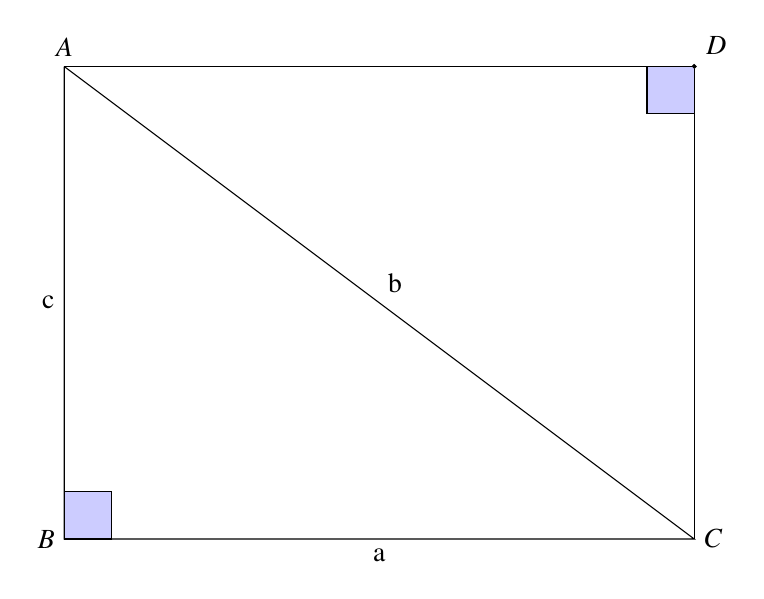
\begin{tikzpicture}
[scale=2,>=stealth,point/.style={draw,circle,fill = black,inner sep=0.5pt},]

%Triangle sides
\def\a{4}
\def\c{3}

%Marking coordiantes
\coordinate [label=above:$A$] (A) at (0,\c);
\coordinate [label=left:$B$] (B) at (0,0);
\coordinate [label=right:$C$] (C) at (\a,0);

%Drawing triangle ABC
\draw (A) -- node[left] {$\textrm{c}$} (B) -- node[below] {$\textrm{a}$} (C) -- node[above,,xshift=2mm] {$\textrm{b}$} (A);

\node (D) at (\a, \c)[point,label=above right:$D$] {};

%Joining AD and CD
\draw (A)--(D);
\draw (C)--(D);

%Drawing and marking angles
\tkzMarkRightAngle[fill=blue!20,size=.3](A,B,C)
\tkzMarkRightAngle[fill=blue!20,size=.3](A,D,C)
\end{tikzpicture}
}
	\end{center}
	\caption{Area of a Right Triangle}
	\label{fig:tri_rect}	
\end{figure}
%
\item Draw Fig. \ref{fig:tri_rect} for $a = 4, c =3$.
\label{const:tri_rect}
\\
\solution Letting
%
\begin{align}
\vec{B} = \myvec{0 \\  0}, 
\vec{D} = \myvec{4 \\  3} 
\label{eq:tri_rect}
\end{align}
%
the python code for  Fig. \ref{fig:tri_rect} is
\begin{lstlisting}
codes/triangle/tri_rect.py
\end{lstlisting}
%
and the equivalent latex-tikz code is
%
\begin{lstlisting}
figs/triangle/tri_rect.tex
\end{lstlisting}

\item
	The area of the two triangles constituting the rectangle is the same.
	\label{ch2_triang_eq}

\item
	The area of the rectangle is the sum of the areas of the two triangles inside.
	\label{ch2_triang_sum}


\item
\label{prob:ch2_triang_area}
	Show that the area of $\Delta ABC$ is $\frac{ac}{2}$

\begin{figure}[!ht]
	\begin{center}
			\resizebox{\columnwidth}{!}{%Code by GVV Sharma
%December 7, 2019
%released under GNU GPL
%Drawing a triangle given 3 sides

\begin{tikzpicture}
[scale=2,>=stealth,point/.style={draw,circle,fill = black,inner sep=0.5pt},]

%Triangle sides
\def\a{6}
\def\b{5}
\def\c{4}
 
%Coordinates of A
%\def\p{{\a^2+\c^2-\b^2}/{(2*\a)}}
\def\p{2.25}
\def\q{{sqrt(\c^2-\p^2)}}

%Labeling points
\node (A) at (\p,\q)[point,label=above right:$A$] {};
\node (B) at (0, 0)[point,label=below left:$B$] {};
\node (C) at (\a, 0)[point,label=below right:$C$] {};

%Foot of perpendicular

\node (D) at (\p,0)[point,label=above right:$D$] {};

%Drawing triangle ABC
\draw (A) -- node[left] {$\textrm{c}$} (B) -- node[below] {$\textrm{a}$} (C) -- node[above,xshift=2mm] {$\textrm{b}$} (A);

%Drawing altitude AD
\draw (A) -- node[left] {$\textrm{h}$}(D);

%Drawing and marking angles
%\tkzMarkAngle[fill=orange!40,size=0.5cm,mark=](A,C,B)
%\tkzMarkAngle[fill=orange!40,size=0.4cm,mark=](D,B,A)
%\tkzMarkAngle[fill=green!40,size=0.5cm,mark=](B,A,C)
%\tkzMarkAngle[fill=green!40,size=0.5cm,mark=](C,B,D)
\tkzMarkRightAngle[fill=blue!20,size=.2](A,D,B)
%\tkzMarkRightAngle[fill=blue!20,size=.2](B,D,A)
%\tkzLabelAngle[pos=0.65](A,C,B){$\theta$}
%\tkzLabelAngle[pos=0.65](A,B,D){$\theta$}
%\tkzLabelAngle[pos=1](B,A,C){\rotatebox{-45}{$\alpha = 90\degree -\theta$}}
%\tkzLabelAngle[pos=0.65](C,B,D){$\alpha$}

\end{tikzpicture}
}
	\end{center}
	\caption{Area of a Triangle}
	\label{fig:tri_sss}	
\end{figure}

\solution From\eqref{ch2_triang_sum},
\begin{equation}
\label{ch2_triang_ar_1}
ar\brak{ABCD} = ar\brak{ACB} + ar\brak{ADB}
\end{equation}
Also from \eqref{ch2_triang_eq},
\begin{equation}
\label{ch2_triang_ar_2}
ar\brak{ACB} = ar\brak{ADB}
\end{equation}
From \eqref{ch2_triang_ar_1} and \eqref{ch2_triang_ar_2},
\begin{align}
2ar\brak{ACB} &= ar\brak{ABCD} = ac \brak{\text{from} \quad \eqref{fig:tri_rect}}
\\
\Rightarrow ar\brak{ACB} &= \frac{ac}{2}
\label{eq:tri_area_rect}
\end{align}

%
\item In Fig. 	\ref{fig:tri_sss}, $AD \perp BC$.  $AD$ is defined as the {\em altitude}.
\item
	Show that the area of $\Delta ABC$ in Fig. 	\ref{fig:tri_sss}	is $\frac{1}{2}ah$. 


\solution In Fig. \ref{fig:tri_sss},
\begin{align}
ar\brak{\Delta ADC} &= \frac{1}{2}hy \\
ar\brak{\Delta ADB} &= \frac{1}{2}hx 
\end{align}
Thus,
\begin{align}
ar\brak{\Delta ABC} &= ar\brak{\Delta ADC} + ar\brak{\Delta ADB} \\
&= \frac{1}{2}hy + \frac{1}{2}hx = \frac{1}{2}h\brak{x+y} \\
&= \frac{1}{2}ah
\end{align}
%
\item Draw Fig. \ref{fig:tri_sss} with $a=6$, $b=5$  and $c=4$.  
\label{const:tri_sss}
\\
\solution Let the vertices of  $\triangle ABC$ and $\vec{D}$ be 
\begin{align}
\label{eq:tri_basic}
\vec{A} = \myvec{p\\q}, \vec{B} = \myvec{0\\0}, \vec{C} = \myvec{a\\0}, \vec{D} = \myvec{p\\0}
\end{align}
%

Then
\begin{align}
\label{eq:c_tricoord}
AB &= \norm{\vec{A}-\vec{B}}^2 = \norm{\vec{A}}^2  = c^2 \quad \because \vec{B} = \vec{0}
\\
\label{eq:a_tricoord}
BC &= \norm{\vec{C}-\vec{B}}^2 = \norm{\vec{C}}^2  = a^2
\\
AC &= \norm{\vec{A}-\vec{C}}^2 =    b^2
\label{eq:b_tricoord}
\end{align}
%
From \eqref{eq:b_tricoord},
\begin{align}
b^2 &=\norm{\vec{A}-\vec{C}}^2 = \norm{\vec{A}-\vec{C}}^T\norm{\vec{A}-\vec{C}}  
\\
&= \vec{A}^T\vec{A}+\vec{C}^T\vec{C}-\vec{A}^T\vec{C} - \vec{C}^T\vec{A} 
\\
&= \norm{\vec{A}}^2 + \norm{\vec{C}}^2 - 2\vec{A}^T\vec{C} \quad \brak{\because \vec{A}^T\vec{C} = \vec{C}^T\vec{A} } 
\label{eq:tri_const_norm_ac}
\\
&= a^2+c^2-2ap
\end{align}
%
yielding
\begin{align}
p&= \frac{a^2+c^2-b^2}{2a}
\end{align}
%
From \eqref{eq:c_tricoord}, 
\begin{align}
\norm{\vec{A}}^2 &= c^2 = p^2+q^2
\\
\implies q&= \pm \sqrt{c^2-p^2}
\end{align}
%
The python code for  Fig. \ref{fig:tri_sss} is
\begin{lstlisting}
codes/triangle/tri_sss.py
\end{lstlisting}
%
and the equivalent latex-tikz code is
%
\begin{lstlisting}
figs/triangle/tri_sss.tex
\end{lstlisting}
\end{enumerate}


\subsection{Sine and Cosine formula}
\renewcommand{\theequation}{\theenumi}
\begin{enumerate}[label=\arabic*.,ref=\thesubsection.\theenumi]
\numberwithin{equation}{enumi}

\item
\label{prob:tri_area_sin}
	Show that the area of $\Delta ABC$ in Fig. 	\ref{fig:tri_sss}	is $\frac{1}{2}ab \sin C$.

\solution We have
%
\begin{equation}
ar\brak{\Delta ABC} = \frac{1}{2}ah = \frac{1}{2}ab\sin C \quad \brak{\because \quad h = b \sin C}.
\label{eq:tri_area_sin}
\end{equation}
%
\item Show that
\begin{align}
\label{eq:sin90}
\sin 90 \degree = 1
\end{align}
%
\begin{figure}[!ht]
\centering
\resizebox{\columnwidth}{!}{%Code by GVV Sharma
%December 6, 2019
%released under GNU GPL
%Drawing a right angled triangle

\begin{tikzpicture}[scale=2]

%Triangle sides
\def\a{4}
\def\c{3}

%Marking coordiantes
\coordinate [label=above:$A$] (A) at (0,\c);
\coordinate [label=left:$B$] (B) at (0,0);
\coordinate [label=right:$C$] (C) at (\a,0);

%Drawing triangle ABC
\draw (A) -- node[left] {$\textrm{c}$} (B) -- node[below] {$\textrm{a}$} (C) -- node[above,,xshift=2mm] {$\textrm{b}$} (A);

%Drawing and marking angles
\tkzMarkAngle[fill=orange!40,size=0.5cm,mark=](A,C,B)
\tkzMarkRightAngle[fill=blue!20,size=.3](A,B,C)
\tkzLabelAngle[pos=0.65](A,C,B){$\theta$}
\end{tikzpicture}
}
\caption{$\sin 90\degree = 1$}
\label{fig:tri_right_angle_area}	
\end{figure}

\solution In Fig. \ref{fig:tri_right_angle_area}, 
using \eqref{eq:tri_area_sin} and \eqref{eq:tri_area_rect}
\begin{align}
ar \brak{\triangle ABC} &= \frac{1}{2}ac \sin B = \frac{1}{2}ac
\\
\implies \sin B &= \sin 90\degree = 1
\end{align}
%
\item Show that
\begin{align}
\label{eq:cos90}
\cos 90 \degree = 1
\end{align}
%
\solution Trivial using \eqref{eq:tri_sin_cos_id}.


\item
	Show that 
	\begin{equation}
	\frac{\sin A}{a} = \frac{\sin B}{b} = \frac{\sin C}{c}
	\end{equation}

\solution Fig. \ref{fig:tri_sss} can be suitably modified to obtain 
\begin{multline}
ar\brak{\Delta ABC} = 
\\
\frac{1}{2}ab\sin C = \frac{1}{s}bc\sin A = \frac{1}{2}ca\sin B
\end{multline}
Dividing the above by $abc$, we obtain
	\begin{equation}
\label{eq:tri_sin_form}
	\frac{\sin A}{a} = \frac{\sin B}{b} = \frac{\sin C}{c}
	\end{equation}
This is known as the sine formula.	
%
\item
In Fig. \ref{fig:tri_cosine_formula}, show that
%
\begin{equation}
\label{eq:tri_cos_form}
\cos A = \frac{b^2+c^2-a^2}{2bc}
\end{equation}
%
\

\begin{figure}[!ht]
	\begin{center}
		
		%
\includegraphics[width=\columnwidth]{./figs/ch2_triang_ar}
		%\vspace*{-10cm}
		\resizebox{\columnwidth}{!}{%Code by GVV Sharma
%December 7, 2019
%released under GNU GPL
%Drawing a triangle given 3 sides

\begin{tikzpicture}
[scale=2,>=stealth,point/.style={draw,circle,fill = black,inner sep=0.5pt},]

%Triangle sides
\def\a{6}
\def\b{5}
\def\c{4}
 
%Coordinates of A
%\def\p{{\a^2+\c^2-\b^2}/{(2*\a)}}
\def\p{2.25}
\def\q{{sqrt(\c^2-\p^2)}}

%Labeling points
\node (A) at (\p,\q)[point,label=above right:$A$] {};
\node (B) at (0, 0)[point,label=below left:$B$] {};
\node (C) at (\a, 0)[point,label=below right:$C$] {};

%Foot of perpendicular

\node (D) at (\p,0)[point,label=above right:$D$] {};

%Drawing triangle ABC
\draw (A) -- node[left] {$\textrm{c}$} (B) -- node[below] {$\textrm{a}$} (C) -- node[above,xshift=2mm] {$\textrm{b}$} (A);

%Drawing altitude AD
\draw (A) -- node[left] {$\textrm{h}$}(D);

\tkzMarkRightAngle[fill=blue!20,size=.2](A,D,B)

\node [below] at ($(B)!0.5!(D)$) {$x$};
\node [below] at ($(C)!0.5!(D)$) {$y$};

\end{tikzpicture}
}
	\end{center}
	\caption{The cosine formula}
	\label{fig:tri_cosine_formula}	
\end{figure}

\solution From Fig. \ref{fig:tri_cosine_formula}, 
%
\begin{align}
a &= x + y = b \cos C + c \cos B.
\end{align}
%
Similarly,
%
\begin{align}
b &= c \cos A + a \cos C \\
c &= b \cos A + a \cos B
\end{align}
%
The above equations can be expressed in matrix form as
%
\begin{equation}
\begin{pmatrix}
0 & c & b \\
c & 0 & a \\
b & a & 0
\end{pmatrix}
\begin{pmatrix}
\cos A \\
\cos B \\
\cos C
\end{pmatrix}
= 
\begin{pmatrix}
a\\
b\\
c
\end{pmatrix}
\end{equation}
%
Using the properties of determinants,
%
\begin{align}
\cos A &= \frac{
\begin{vmatrix}
a & c & b \\
b & 0 & a \\
c & a & 0
\end{vmatrix}
	}
	{
\begin{vmatrix}
0 & c & b \\
c & 0 & a \\
b & a & 0
\end{vmatrix}
	}
	=\frac{ab^2 + ac^2 - a^3}{abc + abc} 
\\
&= \frac{b^2 + c^2 - a^2}{2abc}
\end{align}
%
\item Show that 
%
\begin{align}
\label{eq:trig_id_sin_inc}
\alpha > \beta \implies \sin \alpha > \sin \beta
\end{align}
%

\begin{figure}[!ht]
	\begin{center}
		
		%\includegraphics[width=\columnwidth]{./figs/fig:tri_sin_inc}
		%\vspace*{-10cm}
		\resizebox{\columnwidth}{!}{\begin{tikzpicture}
[scale =3,>=stealth,point/.style = {draw, circle, fill = black, inner sep = 1pt},]

\node (A) at (0,3)[point,label=above :$A$] {};
\node (B) at (3,0)[point,label=below :$B$] {};
\node (C) at (0,0)[point,label=below :$C$] {};
\node (D) at (0,1.5)[point,label=left :$D$] {};
\draw (A)--(B);
\draw (C)--(B);
\draw (A)--(C);
\draw (B)--(D);
\tkzMarkAngle[size=.4](A,B,D);
\tkzMarkAngle[size=.3](D,B,C);
\tkzMarkRightAngle[size=.15](A,C,B);

\node [above] at (1.6,1.5){$c$};
\node [below] at (1.6,0){$a$};
\node [below] at (1.6,1){$l$};
\node [above] at (-0.2,1.5){$b$};
\node [above] at (2.5,0){$\theta_2$};
\node [above] at (2.5,0.3){$\theta_1$};
\end{tikzpicture}}
	\end{center}
	\caption{$\sin \brak{\theta_1+\theta_2} = \sin\theta_1\cos\theta_2 + \cos\theta_1\sin\theta_2$}
	\label{fig:tri_sin_inc}	
\end{figure}
\solution In Fig. \ref{fig:tri_sin_inc}, 	
%
\begin{align}
ar\brak{\triangle ABD} &< ar \brak{\triangle ABC}
\\
\implies \frac{1}{2}lc \sin \theta_1 &<  \frac{1}{2}ac \sin \brak{\theta_1 + \theta_2 }
\\
\implies \frac{l}{a} &< \frac{\sin \brak{\theta_1 + \theta_2 }}{\sin \theta_1}
\\
\text{or, } 1 < \frac{l}{a} &< \frac{\sin \brak{\theta_1 + \theta_2 }}{\sin \theta_1}
\\
\implies \frac{\sin \brak{\theta_1 + \theta_2 }}{\sin \theta_1} > 1
\end{align}
%
from Theorem \ref{them:hyp_largest}. This proves \eqref{eq:trig_id_sin_inc}.
%From \eqref{eq:trig_id_sum_diff3},
%%
%\begin{multline}
% \sin \theta_1 - \sin \theta_2 = 2\sin\brak{\frac{\theta_1-\theta_2}{2}}
%\\
%\times \cos\brak{\frac{\theta_1+\theta_2}{2}} > 0, \because \theta_1-\theta_2 > 0
%\end{multline}
%
\item In a triangle, the side opposite the greater angle is greater.
\begin{figure}[!ht]
	\begin{center}
			\resizebox{\columnwidth}{!}{%Code by GVV Sharma
%December 14, 2019
%released under GNU GPL
%Drawing a triangle given 3 sides

\begin{tikzpicture}
[scale=2,>=stealth,point/.style={draw,circle,fill = black,inner sep=0.5pt},]

%Triangle sides
\def\a{6}
\def\b{5}
\def\c{4}
 
%Coordinates of A
%\def\p{{\a^2+\c^2-\b^2}/{(2*\a)}}
\def\p{2.25}
\def\q{{sqrt(\c^2-\p^2)}}

%Labeling points
\node (A) at (\p,\q)[point,label=above right:$A$] {};
\node (B) at (0, 0)[point,label=below left:$B$] {};
\node (C) at (\a, 0)[point,label=below right:$C$] {};


%Drawing triangle ABC
\draw (A) -- node[left] {$\textrm{c}$} (B) -- node[below] {$\textrm{a}$} (C) -- node[above,xshift=2mm] {$\textrm{b}$} (A);
\end{tikzpicture}
}
	\end{center}
	\caption{Side opposite the greater angle is greater}
	\label{fig:tri_ang_side}	
\end{figure}
\\
\solution In Fig. 	\ref{fig:tri_ang_side},	let
%
\begin{align}
\angle B > \angle C
\end{align}
%
Then, using the sine formula,
%
\begin{align}
\frac{\sin B}{b} &=\frac{\sin C}{c}
\\
\implies   \frac{\sin B}{\sin C} &= \frac{b}{c} > 1
\end{align}
using \eqref{eq:trig_id_sin_inc}.


\end{enumerate}


\subsection{Hero's formula}
\renewcommand{\theequation}{\theenumi}
\begin{enumerate}[label=\arabic*.,ref=\thesubsection.\theenumi]
\numberwithin{equation}{enumi}

\item Find Hero's formula for the area of a triangle.
\\
\solution 
%In Fig. \ref{fig:rt_triangle}, from Baudhayana's theorem, 
%\begin{align}
%\label{eq:tri_geo_baudh}
%b^2 = a^2+c^2 &
%\\
%=b^2\cos^2C+b^2\sin^2C &
%\\
%\implies \cos^2C+\sin^2C &= 1
%\end{align}
%
%In Fig. \ref{fig:tri_const_ex_cos_form}, 
From \eqref{prob:tri_area_sin}, the area of $\triangle ABC$ is 
{\footnotesize
\begin{align}
\label{eq:tri_geo_area_sin_form}
 \frac{1}{2}ab\sin C
%\\
&=\frac{1}{2}ab\sqrt{1-\cos^2C} 
\quad \brak{\text{from } \eqref{eq:tri_sin_cos_id}
%\eqref{eq:tri_geo_baudh}
}
\\
&=\frac{1}{2}ab\sqrt{1-\brak{\frac{a^2+b^2-c^2}{2ab}}^2} \brak{\text{from } \eqref{eq:tri_cos_form}
}
\\
&=\frac{1}{4}\sqrt{\brak{2ab}^2-\brak{a^2+b^2-c^2}}
\\
&=\frac{1}{4}\sqrt{\brak{2ab+a^2+b^2-c^2}\brak{2ab-a^2-b^2+c^2}}
\\
&= \frac{1}{4}\sqrt{\cbrak{\brak{a+b}^2-c^2}\cbrak{c^2-\brak{a-b}^2}}
\\
&= \frac{1}{4}\sqrt{\brak{a+b+c}\brak{a+b-c}\brak{a+c-b}\brak{b+c-a}}
\label{eq:tri_ex_hero_temp}
\end{align}
}
Substituting 
%
\begin{align}
s=\frac{a+b+c}{2}
\end{align}
%
in \eqref{eq:tri_ex_hero_temp}, the area of $\triangle ABC$ is 
%
\begin{align}
\label{eq:tri_area_hero}
\sqrt{s\brak{s-a}\brak{s-b}\brak{s-c}}
\end{align}
%
This is known as Hero's formula.
\item Find the area of $\triangle ABC$ in Fig. \ref{fig:tri_rect}.
\\
\solution The desired are is computed using \eqref{eq:tri_area_hero} by the following 
the python code.
\begin{lstlisting}
codes/triangle/tri_area_hero.py
\end{lstlisting}
%

\item Show that the sum of two sides of a triangle is always greater than the third side.
\\
\solution In \eqref{eq:tri_area_hero}, all terms under the square roots should be positive.  Hence,
%
\begin{align}
\label{eq:tri_hero_ineq}
\begin{split}
s-a &>0
\\
s-b &>0
\\
s-c &>0
\end{split}
\end{align}
resulting in 
%
\begin{align}
\begin{split}
\label{eq:tri_sum_ineq}
b+c &>a
\\
c+a &>b
\\
a+b &>c
\end{split}
\end{align}
\end{enumerate}




\section{Circumcentre}
\subsection{Locating the Circumcentre}
%%
%\subsection{Perpendicular Bisectors}
\renewcommand{\theequation}{\theenumi}
\begin{enumerate}[label=\arabic*.,ref=\thesubsection.\theenumi]
\numberwithin{equation}{enumi}

\item Find a point $\vec{O}$ that is equidistant from the vertices of $\triangle ABC$ for $a = 5, b = 6, c = 4$.
%
\solution Let $\vec{O}$ be the desired point.  Then,
\begin{align}
\label{eq:tri_ccentre_def}
\norm{\vec{A}-\vec{O}} = \norm{\vec{B}-\vec{O}} = 
\norm{\vec{C}-\vec{O}} = R
%\\
%\implies \norm{\vec{x}-\vec{O}}^2 &=\brak{\vec{x}-\vec{O}}^T\brak{\vec{x}-\vec{O}} = R^2
\end{align}
From \eqref{eq:tri_ccentre_def},
\begin{align}
\label{eq:circle_const_AB}
\norm{\vec{A}-\vec{O}}^2 - \norm{\vec{B}-\vec{O}}^2  = 0
\end{align}
\begin{multline}
\implies \brak{\vec{A}-\vec{O}}^T\brak{\vec{A}-\vec{O}} 
\\
- \brak{\vec{B}-\vec{O}}^T\brak{\vec{B}-\vec{O}} = 0
\end{multline}
%
which can be simplified as
\begin{align}
\label{eq:circle_const_chord_ab}
\brak{\vec{A}-\vec{B}}^T\vec{O} =   \frac{\norm{\vec{A}}^2- \norm{\vec{B}}^2}{2}
\end{align}
Similarly,
\begin{align}
\label{eq:circle_const_chord_bc}
\brak{\vec{B}-\vec{C}}^T\vec{O} =   \frac{\norm{\vec{B}}^2- \norm{\vec{C}}^2}{2}
\end{align}
%
\eqref{eq:circle_const_chord_ab} and \eqref{eq:circle_const_chord_ab}, can be combined to form the matrix equation 
%
\begin{align}
\vec{N}^T\vec{O} &= \vec{c}
\\
\implies \vec{O} &= \vec{N}^{-T} \vec{c}
\label{eq:circle_const_chord_mat}
\end{align}
%
where 
%
\begin{align}
%\label{eq:circle_const_chord_mat}
\vec{N} &= \myvec{\vec{A}-\vec{B} & \vec{B}-\vec{C}}
\\
\vec{c} &= \frac{1}{2}\myvec{\norm{\vec{A}}^2- \norm{\vec{B}}^2 \\ \norm{\vec{B}}^2- \norm{\vec{C}}^2}
\end{align}
%
$\vec{O}$ can be computed using 
%
the python code below
%
\begin{lstlisting}
codes/circle/tri_ccentre.py
\end{lstlisting}
%
and the equivalent latex-tikz code to draw Fig. \ref{fig:tri_ccentre} is
%
\begin{lstlisting}
figs/triangle/tri_ccentre.tex
\end{lstlisting}
%
\begin{figure}[!ht]
	\begin{center}
		
		\resizebox{\columnwidth}{!}{%Code by GVV Sharma
%December 9, 2019
%released under GNU GPL
%Locating the circumcentre

\begin{tikzpicture}
[scale=2,>=stealth,point/.style={draw,circle,fill = black,inner sep=0.5pt},]

%Triangle sides
\def\a{5}
\def\b{6}
\def\c{4}
 
%Coordinates of A
%\def\p{{\a^2+\c^2-\b^2}/{(2*\a)}}
\def\p{0.5}
\def\q{{sqrt(\c^2-\p^2)}}

%Labeling points
\node (A) at (\p,\q)[point,label=above right:$A$] {};
\node (B) at (0, 0)[point,label=below left:$B$] {};
\node (C) at (\a, 0)[point,label=below right:$C$] {};

%Circumcentre

\node (O) at (2.5,1.70084013)[point,label=above right:$O$] {};

%Drawing triangle ABC
\draw (A) -- node[left] {$\textrm{c}$} (B) -- node[below] {$\textrm{a}$} (C) -- node[above,yshift=2mm] {$\textrm{b}$} (A);
%Drawing OA, OB, OC
\draw (O) -- node[left] {$\textrm{R}$} (A);
\draw (O) -- node[below] {$\textrm{R}$} (B);
\draw (O) -- node[below] {$\textrm{R}$} (C);

\tkzMarkAngle[fill=blue!50,size=.3](C,B,O)
\tkzMarkAngle[fill=blue!50,size=.3](O,C,B)


\tkzMarkAngle[fill=red!50](O,A,C)
\tkzMarkAngle[fill=red!50](A,C,O)


\tkzMarkAngle[fill=orange!50,size=.3](B,A,O)
\tkzMarkAngle[fill=orange!50,size=.3](O,B,A)

\tkzLabelAngle[pos=0.5](O,C,B){$\theta_1$}
\tkzLabelAngle[pos=0.5](O,B,C){$\theta_1$}
\tkzLabelAngle[pos=0.5](O,A,B){$\theta_2$}
\tkzLabelAngle[pos=0.5](O,B,A){$\theta_2$}
\tkzLabelAngle[pos=1.5](O,A,C){$\theta_3$}
\tkzLabelAngle[pos=1.5](O,C,A){$\theta_3$}

\end{tikzpicture}
}
	\end{center}
	\caption{Circumcentre $O$ of $\triangle ABC$}
	\label{fig:tri_ccentre}	
\end{figure}
%
\item In $\triangle OBC$, $OB = OC = R$.  Such a triangle is known as an {\em isoceles triangle}.
%
\item Show that $\angle OBC = \angle OCB$.  In an isoceles triangle, opposite sides and corresponding opposite angles are equal.
\label{prob:tri_ang_side_eq}
\\
\solution Using the sine formula in \eqref{eq:tri_sin_form},%
\begin{align}
\frac{\sin \angle OBC}{R} &= \frac{\sin \angle OCB}{R}
\\
\implies \sin \angle OBC &= \sin \angle OCB
\end{align}
%
\item  Show that $\angle BOC = 2\angle A$.
\label{prob:tri_ccentre_subtend}
%
\\
\solution In Fig. \ref{fig:tri_ccentre}, 
%
\begin{align}
%
\label{eq:tri_ccentre_A23}
A &= \theta_2+\theta_3
\\
B &= \theta_1+\theta_2
\\
C &= \theta_3+\theta_1
\\
\implies 2\brak{\theta_1+\theta_2+\theta_3} &= A+B+C =180\degree
\\
\implies \theta_1+\theta_2+\theta_3 &= 90\degree
\label{eq:tri_ccentre_sum_123}
\end{align}
%
From \eqref{eq:tri_ccentre_A23} and \eqref{eq:tri_ccentre_sum_123},
%
\begin{align}
%
\label{eq:tri_ccentre_A1}
A &= 90\degree - \theta_1
\end{align}
%
Also, in $\triangle OBC$, all angles add up to $180\degree$.  Hence, 
%
\begin{align}
\angle BOC + 2\theta_1 &= 180\degree
\\
\implies \angle BOC &= 180\degree - 2\theta_1 = 2 \brak{90\degree - \theta_1}
%\\
%&
= 2\angle A
\end{align}
%
upon substituting from \eqref{eq:tri_ccentre_A1}.
%
\item Let $\vec{D}$ be the mid point of $BC$.  Show that $OD \perp BC$.
\label{prob:tri_perp_bisect}
%
\\
\solution From \eqref{eq:circle_const_chord_bc}, 
%
\begin{align}
\brak{\vec{B}-\vec{C}}^T\vec{O} &=   \frac{\norm{\vec{B}}^2- \norm{\vec{C}}^2}{2}
\\
\implies \brak{\vec{B}-\vec{C}}^T\vec{O} &=   \frac{1}{2}\brak{\vec{B}- \vec{C}}^T\brak{\vec{B}+ \vec{C}}
\\
\implies \brak{\vec{B}-\vec{C}}^T&\brak{\vec{O} - \frac{\vec{B}+\vec{C}}{2}} = 0
\\
\text{or, } \brak{\vec{B}-\vec{C}}^T&\brak{\vec{O} - \vec{D}} = 0
\end{align}
%
$\because \vec{D} = \frac{\vec{B}+\vec{C}}{2}$ is the mid point of $BC$.  From \eqref{eq:tri_baudh_orth} we then conclude that $OD \perp BC$.
%
\item Perpendicular bisectors of a triangle meet at the circumcentre.
\end{enumerate}


\subsection{Finding the Circumradius}
%%
%\subsection{Perpendicular Bisectors}
\renewcommand{\theequation}{\theenumi}
\begin{enumerate}[label=\arabic*.,ref=\thesubsection.\theenumi]
\numberwithin{equation}{enumi}

\item Show that 
\begin{align}
\label{eq:tri_crad_R}
\frac{a}{\sin A} = \frac{b}{\sin B} = \frac{c}{\sin C} = 2R.
\end{align}
%
\solution In $\triangle OBC$, using the cosine formula, 
\begin{align}
\cos 2A = \frac{R^2+R^2 - a^2}{2R^2} = 1 -\frac{a^2}{2R^2}
\label{eq:crad_cos2a}
\end{align}
%
Using the sine formula, 
\begin{align}
\frac{\sin 2A}{a} &= \frac{\sin \theta_1}{R} = \frac{\sin\brak{90\degree- A}}{R}
\\
\implies \sin 2A &= \frac{a\cos A}{R}
\label{eq:crad_sin2a}
\end{align}
%
from \eqref{eq:tri_ccentre_A1} and \eqref{eq:tri_baudh_comp}.	Using \eqref{eq:tri_sin_cos_id}, 
\begin{align}
\cos^2 2A + \sin^2 2A&= 1
\\
\implies \brak{1 -\frac{a^2}{2R^2}}^2 + \brak{\frac{a\cos A}{R}}^2 &= 1
\end{align}
%
upon substituting from \eqref{eq:crad_cos2a}  and \eqref{eq:crad_sin2a}.  Letting
%
\begin{align}
\label{eq:tri_crad_x}
x = \brak{\frac{a}{R}}^2,
\end{align}
%
in the previous equation yields
%
\begin{align}
 \brak{1 -\frac{x}{2}}^2 + x\cos^2 A&= 1
\\
\implies 1 - \frac{x^2}{4} -x + x\cos^2 A&= 1
\\
\implies x\brak{1-\cos^2 A} - \frac{x^2}{4} &= 0
\end{align}
%
From \eqref{eq:tri_sin_cos_id}, the above equation can be expressed as
%
\begin{align}
x\sin^2 A - \frac{x^2}{4} &= 0
\\
\implies x\brak{\sin^2 A - \frac{x}{4}} &= 0
\\
\text{or, } \frac{x}{4} - \sin^2 A &=0
\end{align}
%
$\because x \ne 0$.  Thus, substituting from \eqref{eq:tri_crad_x},
\begin{align}
x = \brak{\frac{a}{R}}^2 &= 4 \sin^2 A 
\\
\implies \frac{a}{R} &= 2\sin A,
\\
\text{or, }\quad \frac{a}{\sin A} = 2R
%\label{eq:circ_chord_len}
\end{align}
%
\item Show that 
\label{eq:cos2x}
\begin{align}
\cos 2A &= 1 -2\sin^2 A = 2\cos^2 A - 1 
\\
&= \cos^2 A - \sin^2A \quad \text{ and }
\\
\sin 2A &= 2 \sin A \cos A
\label{eq:sin2x}
\end{align}
\item Find $R$.
\\
\solution From \eqref{eq:tri_area_sin}, 
\begin{align}
ar\brak{\triangle ABC} = \frac{1}{2}bc \sin A = \frac{abc}{4R}&
\\
\implies R = \frac{abc}{4s\sqrt{\brak{s-a}\brak{s-b}\brak{s-c}}}&
\end{align}
%
upon substituting from \eqref{eq:tri_crad_R} and using Hero's formula.
%
\item Show that
%
\begin{align}
\label{eq:circ_area_chord}
ar\brak{\triangle OBC} = \frac{1}{2}R^2\sin 2A
\end{align}
%
\item Find the circumradius of $\triangle ABC$ for $a = 5, b = 6, c = 4$.
%
\\
\solution The following python code calculates the circumradius
\begin{lstlisting}
codes/circle/tri_cradius.py
\end{lstlisting}


\end{enumerate}

\subsection{Drawing the Circumcircle}
%%
\renewcommand{\theequation}{\theenumi}
\begin{enumerate}[label=\arabic*.,ref=\thesubsection.\theenumi]
\numberwithin{equation}{enumi}

\item In Fig. \ref{fig:tri_ccentre}, points $\vec{A}, \vec{B}, \vec{C}$  are at a distance $R$ from $\vec{O}$.  Trace all such points. The locus of such points is defined as a {\em circle}.
%
\\
\solution This is done by the following python code
%
\begin{lstlisting}
codes/circle/tri_ccircle.py
\end{lstlisting}
%
and the equivalent latex-tikz code to draw Fig. \ref{fig:tri_ccircle} is
%
\begin{lstlisting}
figs/triangle/tri_ccircle.tex
\end{lstlisting}

\begin{figure}[!ht]
	\begin{center}
		
		\resizebox{\columnwidth}{!}{%Code by GVV Sharma
%December 9, 2019
%released under GNU GPL
%Locating the circumcentre

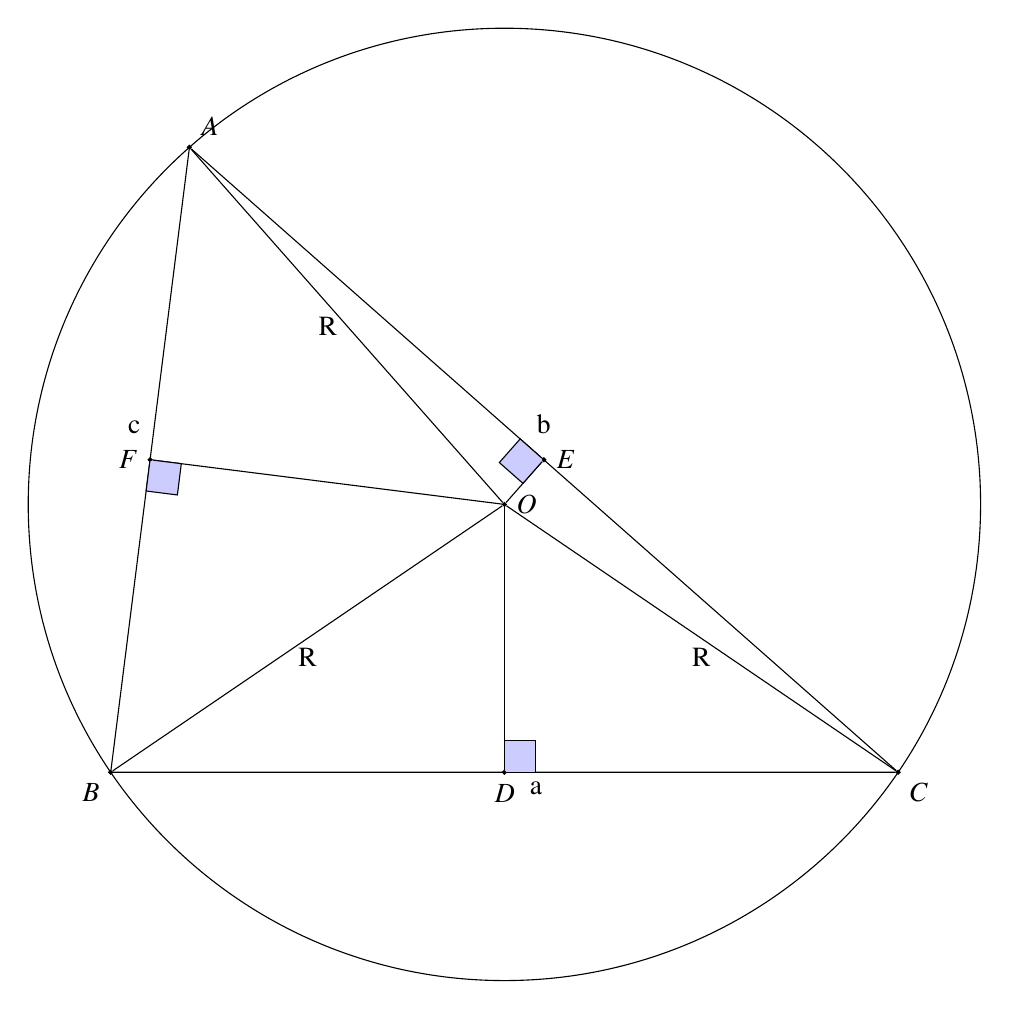
\begin{tikzpicture}
[scale=2,>=stealth,point/.style={draw,circle,fill = black,inner sep=0.5pt},]

%Triangle sides
\def\a{5}
\def\b{6}
\def\c{4}
\def\R{3.023715784073818}
 
%Coordinates of A
%\def\p{{\a^2+\c^2-\b^2}/{(2*\a)}}
\def\p{0.5}
\def\q{{sqrt(\c^2-\p^2)}}

% Vertices
\node (A) at (\p,\q)[point,label=above right:$A$] {};
\node (B) at (0, 0)[point,label=below left:$B$] {};
\node (C) at (\a, 0)[point,label=below right:$C$] {};

% Mid points
\node (D) at ($(B)!0.5!(C)$)[point,label=below:$D$] {};
\node (E) at ($(C)!0.5!(A)$)[point,label=right:$E$] {};
\node (F) at ($(B)!0.5!(A)$)[point,label=left:$F$] {};

%Circumcentre

\node (O) at (2.5,1.70084013)[point,label=right:$O$] {};

%Drawing triangle ABC
\draw (A) -- node[above left, yshift=2mm] {$\textrm{c}$} (B) -- node[below right, xshift = 2mm] {$\textrm{a}$} (C) -- node[above,yshift=2mm] {$\textrm{b}$} (A);
%Drawing OA, OB, OC
\draw (O) -- node[left] {$\textrm{R}$} (A);
\draw (O) -- node[below] {$\textrm{R}$} (B);
\draw (O) -- node[below] {$\textrm{R}$} (C);

%Drawing OD, OE, OF
\draw (O) --  (D);
\draw (O) --  (E);
\draw (O) --  (F);


%Drawing circumcircle
\draw (O) circle (\R);

\tkzMarkRightAngle[fill=blue!20,size=.2](O,D,C)
\tkzMarkRightAngle[fill=blue!20,size=.2](O,E,A)
\tkzMarkRightAngle[fill=blue!20,size=.2](O,F,B)

\end{tikzpicture}
}
	\end{center}
	\caption{Circumcircle of $\triangle ABC$}
	\label{fig:tri_ccircle}	
\end{figure}
%
\item Line segements joining any two points on the circle are defined to be {\em chords}. The sides of $\triangle ABC$ are chords of the circle in 	\eqref{fig:tri_ccircle}	

\item From  \eqref{prob:tri_perp_bisect}, it is established that the line segment joining the centre of a circle to the mid point of a chord bisects the chord.
\item From \eqref{prob:tri_ccentre_subtend}, it is clear that the angle subtended by a chord at the centre of the circle is twice the angle subtended at any point on the circle.
\label{them:tri_ccentre_subtend}
%

\end{enumerate}



\section{Incentre}
\subsection{Locating the Incentre}
%%
%\subsection{Perpendicular Bisectors}
\renewcommand{\theequation}{\theenumi}
\begin{enumerate}[label=\arabic*.,ref=\thesubsection.\theenumi]
\numberwithin{equation}{enumi}

\item Find a point $\vec{O}$ that is equidistant from the sides of $\triangle ABC$ for $a = 5, b = 6, c = 4$. Here, distance means the perpendicular distanace.
%
\solution Let $\vec{I}$ be the desired point and  $\vec{D}, \vec{E}, \vec{F}$ are on  $BC, CA, AB$ such that $ID \perp BC, IE \perp CA, IF \perp AB$ and $ID = IE = IF = r$, then, applying \eqref{eq:tri_baudh} in $\triangle s$ $IDB$ and $IEB$,
\begin{align}
\label{eq:tri_icentre_baudhd}
\begin{split}
IB^2 &= ID^2+BD^2 = r^2 + BD^2 
\\
IB^2 &= IF^2+BF^2 = r^2 + BF^2
\end{split}
\end{align}
From the above, it is obvious that $BD = BF$. Similarly, $AE = AF, CD = CF$.  Denoting these lengths as $x, y$ and $z$, as shown in Fig. \ref{fig:tri_icentre},
%
\begin{align}
x + y = a
y+z = b
x + z = c
\end{align}
%
which can be expressed as the matrix equation
%
\begin{align}
\myvec{
1 & 1 & 0
\\
0 & 1 & 1
\\
1 & 0 & 1
}
\myvec{x \\ y \\ z}
=
\myvec{a\\b\\c}
\label{eq:tri_icentre_mat}
\end{align}
%
Section formula can be used to compute 
\begin{align}
\vec{D} = \frac{x\vec{C}+y\vec{B}}{x+y}
\\
\vec{E} = \frac{y\vec{A}+z\vec{C}}{y+z}
\\
\vec{F} = \frac{z\vec{B}+x\vec{A}}{z+x}
\end{align}
%
Note that $\vec{I}$ is the circumcentre of $\triangle DEF$.  Thus, \eqref{eq:circle_const_chord_mat} can be used to compute $\vec{I}$.  
%
This is done by the python code below
%
\begin{lstlisting}
codes/circle/tri_icentre.py
\end{lstlisting}
%
and the equivalent latex-tikz code to draw Fig. \ref{fig:tri_icentre} is
%
\begin{lstlisting}
figs/circle/tri_icentre.tex
\end{lstlisting}
%
\begin{figure}[!ht]
	\begin{center}
		
		\resizebox{\columnwidth}{!}{%Code by GVV Sharma
%December 10, 2019
%released under GNU GPL
%Locating the incentre

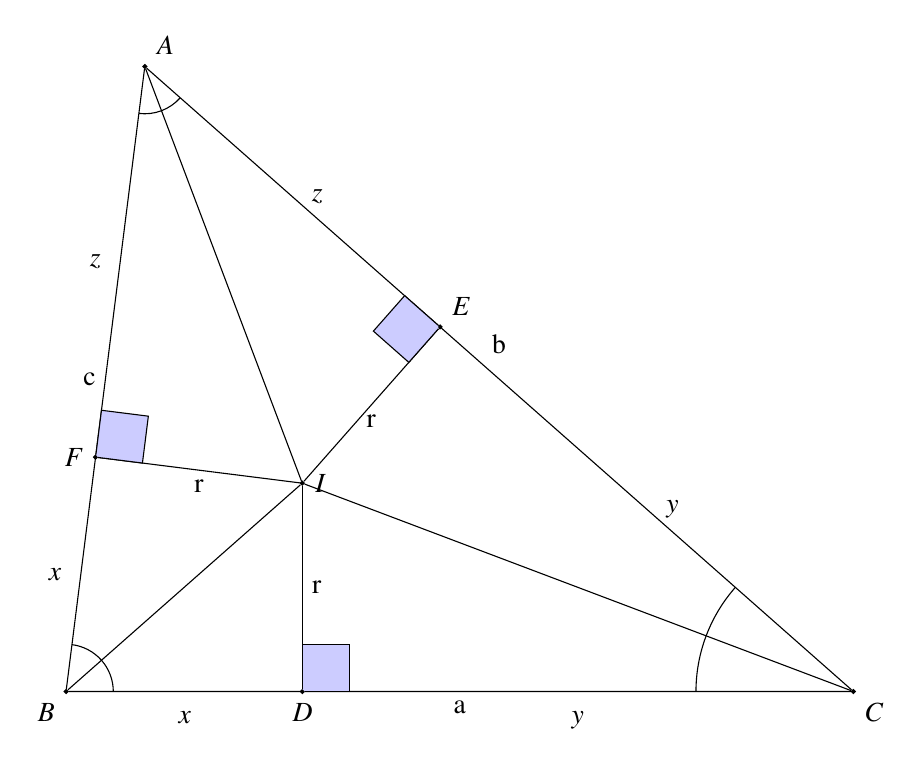
\begin{tikzpicture}
[scale=2,>=stealth,point/.style={draw,circle,fill = black,inner sep=0.5pt},]

%Triangle sides
\def\a{5}
\def\b{6}
\def\c{4}
 
%Coordinates of A
%\def\p{{\a^2+\c^2-\b^2}/{(2*\a)}}
\def\p{0.5}
\def\q{{sqrt(\c^2-\p^2)}}

%Labeling points
\node (A) at (\p,\q)[point,label=above right:$A$] {};
\node (B) at (0, 0)[point,label=below left:$B$] {};
\node (C) at (\a, 0)[point,label=below right:$C$] {};

%Circumcentre

\node (I) at (1.5,1.32287566)[point,label=right:$I$] {};
\node (D) at (1.5,0)[point,label=below:$D$] {};
\node (E) at (2.375,2.3150324)[point,label=above right:$E$] {};
\node (F) at (0.1875,1.48823511)[point,label=left:$F$] {};

%Drawing triangle ABC
\draw (A) -- node[left] {$\textrm{c}$} (B) -- node[below] {$\textrm{a}$} (C) -- node[above,yshift=2mm] {$\textrm{b}$} (A);
%Drawing OA, OB, OC
\draw (I) --  (A);
\draw (I) --  (B);
\draw (I) --  (C);

%Drawing OD, OE, OF
\draw (I) -- node[right] {$\textrm{r}$} (D);
\draw (I) -- node[below] {$\textrm{r}$} (E);
\draw (I) -- node[below] {$\textrm{r}$} (F);

\tkzMarkAngle[fill=green!60,size=.3](I,B,F)
\tkzMarkAngle[fill=green!40,size=.3](D,B,I)
%
%
\tkzMarkAngle[fill=red!60,size=.3](F,A,I)
\tkzMarkAngle[fill=red!40,size=.3](I,A,E)


\tkzMarkAngle[fill=orange!60](E,C,I)
\tkzMarkAngle[fill=orange!40](I,C,D)
%
\tkzMarkRightAngle[fill=blue!20,size=.3](A,E,I)
\tkzMarkRightAngle[fill=blue!20,size=.3](A,F,I)
\tkzMarkRightAngle[fill=blue!20,size=.3](I,D,C)

%Labeling x,y,z
\node (x1) at ($(B)!0.5!(D)$)[label=below:$x$] {};
\node (x2) at ($(B)!0.5!(F)$)[label=left:$x$] {};
\node (y1) at ($(C)!0.5!(D)$)[label=below:$y$] {};
\node (y2) at ($(C)!0.5!(E)$)[label=right:$y$] {};
\node (z1) at ($(A)!0.5!(E)$)[label=right:$z$] {};
\node (z2) at ($(A)!0.5!(F)$)[label=left:$z$] {};


\end{tikzpicture}
}
	\end{center}
	\caption{Incentre $I$ of $\triangle ABC$}
	\label{fig:tri_icentre}	
\end{figure}
%
\item $r$ is known as the {\em inradius} of $\triangle ABC$.  Find $r$ for  the given values of $a,b,c$.
\\
\solution From Fig. \ref{fig:tri_icentre}
%
\begin{align}
\because ar\brak{ABC} &= ar\brak{IBC}+ar\brak{ICA}+ar\brak{IAB}
\\
&=\frac{1}{2}ra+\frac{1}{2}rb+\frac{1}{2}rc = \frac{a+b+c}{2}r,
\\
r &= \frac{\sqrt{s\brak{s-a}\brak{s-b}\brak{s-c}}}{s}
\end{align}
%
using Hero's formula.
%
The following python code computes the {\em inradius}
%
\begin{lstlisting}
codes/circle/tri_iradius.py
\end{lstlisting}

\end{enumerate}


\subsection{Drawing the Incircle}
%%
\renewcommand{\theequation}{\theenumi}
\begin{enumerate}[label=\arabic*.,ref=\thesubsection.\theenumi]
\numberwithin{equation}{enumi}

\item In Fig. \ref{fig:tri_icentre}, points $\vec{D}, \vec{E}, \vec{F}$  are at a distance $r$ from $\vec{I}$.  The circle with centre $\vec{I}$ through these points is known as the {\em incircle}. Draw the incircle of $\triangle ABC$.
%
\\
\solution This is done by the following python code
%
\begin{lstlisting}
codes/circle/tri_icircle.py
\end{lstlisting}
%
and the equivalent latex-tikz code to draw Fig. \ref{fig:tri_icircle} is
%
\begin{lstlisting}
figs/triangle/tri_icircle.tex
\end{lstlisting}

\begin{figure}[!ht]
	\begin{center}
		
		\resizebox{\columnwidth}{!}{%Code by GVV Sharma
%December 10, 2019
%released under GNU GPL
%Drawing the incircle

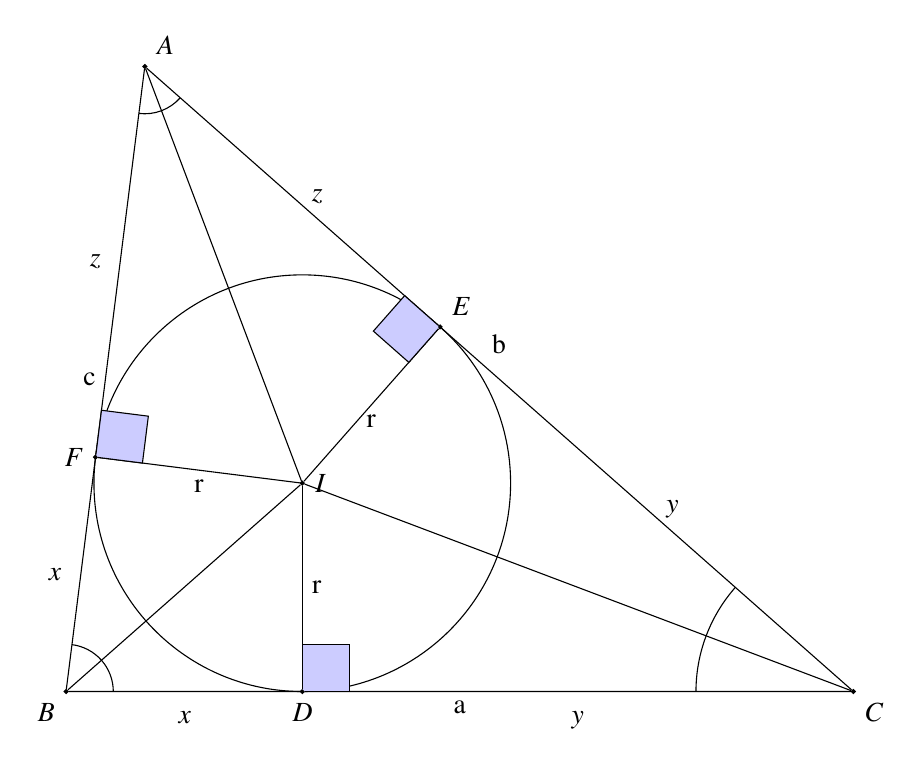
\begin{tikzpicture}
[scale=2,>=stealth,point/.style={draw,circle,fill = black,inner sep=0.5pt},]

%Triangle sides
\def\a{5}
\def\b{6}
\def\c{4}

%Inradius
\def\r{1.3228756555322954}
 
%Coordinates of A
%\def\p{{\a^2+\c^2-\b^2}/{(2*\a)}}
\def\p{0.5}
\def\q{{sqrt(\c^2-\p^2)}}

%Labeling points
\node (A) at (\p,\q)[point,label=above right:$A$] {};
\node (B) at (0, 0)[point,label=below left:$B$] {};
\node (C) at (\a, 0)[point,label=below right:$C$] {};

%Circumcentre

\node (I) at (1.5,1.32287566)[point,label=right:$I$] {};
\node (D) at (1.5,0)[point,label=below:$D$] {};
\node (E) at (2.375,2.3150324)[point,label=above right:$E$] {};
\node (F) at (0.1875,1.48823511)[point,label=left:$F$] {};

%Drawing triangle ABC
\draw (A) -- node[left] {$\textrm{c}$} (B) -- node[below] {$\textrm{a}$} (C) -- node[above,yshift=2mm] {$\textrm{b}$} (A);
%Drawing OA, OB, OC
\draw (I) --  (A);
\draw (I) --  (B);
\draw (I) --  (C);

%Drawing OD, OE, OF
\draw (I) -- node[right] {$\textrm{r}$} (D);
\draw (I) -- node[below] {$\textrm{r}$} (E);
\draw (I) -- node[below] {$\textrm{r}$} (F);

%Drawing Incircle
\draw (I) circle (\r);



\tkzMarkAngle[fill=green!60,size=.3](I,B,F)
\tkzMarkAngle[fill=green!40,size=.3](D,B,I)
%
%
\tkzMarkAngle[fill=red!60,size=.3](F,A,I)
\tkzMarkAngle[fill=red!40,size=.3](I,A,E)


\tkzMarkAngle[fill=orange!60](E,C,I)
\tkzMarkAngle[fill=orange!40](I,C,D)
%
\tkzMarkRightAngle[fill=blue!20,size=.3](A,E,I)
\tkzMarkRightAngle[fill=blue!20,size=.3](A,F,I)
\tkzMarkRightAngle[fill=blue!20,size=.3](I,D,C)

%Labeling x,y,z
\node (x1) at ($(B)!0.5!(D)$)[label=below:$x$] {};
\node (x2) at ($(B)!0.5!(F)$)[label=left:$x$] {};
\node (y1) at ($(C)!0.5!(D)$)[label=below:$y$] {};
\node (y2) at ($(C)!0.5!(E)$)[label=right:$y$] {};
\node (z1) at ($(A)!0.5!(E)$)[label=right:$z$] {};
\node (z2) at ($(A)!0.5!(F)$)[label=left:$z$] {};


\end{tikzpicture}
}
	\end{center}
	\caption{Circumcircle of $\triangle ABC$}
	\label{fig:tri_icircle}	
\end{figure}
%
\item Sides $AB, BC$ and $CA$ touch the circle at exactly one point.  Such lines are known as {\em tangents} to the circle.
\item Tangents to the circle are perpendicular to the radius at the point of contact.
\item From \eqref{eq:tri_icentre_baudhd}, it is  obvious that tangents to the circle from a given point are equal.
%

\end{enumerate}


\subsection{Congruent Triangles}
%%
\renewcommand{\theequation}{\theenumi}
\begin{enumerate}[label=\arabic*.,ref=\thesubsection.\theenumi]
\numberwithin{equation}{enumi}

\item
RHS:	For two right angled triangles, if the hypotenuse and one of the sides are equal, show that the triangles are congruent.
\\
\solution In $\triangle$s $IDB$ and $IFB$ in  Fig. \ref{fig:tri_icentre},  $ID\perp BC, IF\perp AB, IB$ is a common side and $ID = IF$, i.e. both triangles are right angled, have the same hypotenuse and one equal leg.  This information was sufficient to show that $BD = BF$.  Similarly, it can be shown that all angles of both triangles are equal.  Such triangles are known as {\em congruent} triangles and denoted by $\triangle IDB \cong \triangle IEB$.
\item Show that $IA, IB, IC$ bisect the angles $A, B$ and $C$ respectively.  
\item Angle bisectors of $\triangle ABC$ meet at the incentre $\vec{I}$.

\item
To show that two triangles are congruent, it is sufficient to show that some corresponding angles and sides are equal.  Sine and cosine formulae are sufficient to show that two triangles are congruent.



\item
SSS:	Show that if the corresponding sides of three triangles are equal, the triangles are congruent.

\item
ASA:	Show that if two angles and any one side  are equal in corresponding triangles, the triangles are congruent.

\item
SAS:	Show that if two sides and the angle between them are equal in corresponding triangles, the triangles are congruent.%

\end{enumerate}



\section{Medians of a Triangle}
%
\subsection{Median}
\renewcommand{\theequation}{\theenumi}
\begin{enumerate}[label=\arabic*.,ref=\thesubsection.\theenumi]
\numberwithin{equation}{enumi}

\item	The line AD in Fig. \ref{ch2_median_def} that divides the side $a$ in two equal halfs is known as the median.

\begin{figure}[!ht]
	\begin{center}
		
		%
\includegraphics[width=\columnwidth]{./figs/ch2_median_def}
		%\vspace*{-10cm}
		\resizebox{\columnwidth}{!}{\begin{tikzpicture}
[scale=2,>=stealth,point/.style={draw,circle,fill = black,inner sep=0.5pt},]

\node (D) at (0, 0)[point,label=below :$D$] {};
\node (A) at (0, 3)[point,label=above :$A$]{};
\node (B) at (-3, 0)[point,label=below left:$B$]{};
\node (C) at (3, 0)[point,label=below right:$C$]{};

\draw (D)--(B);
\draw (B)--(A);
\draw (A)--(C);
\draw (C)--(D);
\draw (D)--(A);

\node [below] at (0,-0.3) {$a$};
\node [below] at (-1.5,0) {$a/2$};
\node [below] at (1.5, 0) {$a/2$};
\node [above] at (-1.5,1.5){$c$};
\node [above] at (1.5,1.5){$b$};

\end{tikzpicture}}
	\end{center}
	\caption{Median of a Triangle}
	\label{ch2_median_def}	
\end{figure}

\item
	Show that the median $AD$ in Fig. \ref{ch2_median_def} divides  $\Delta ABC$ into triangles $ADB$ and $ADC$ that have equal area.

\solution We have
%
\begin{align}
ar \brak{\Delta ADB} &= \frac{1}{2}\frac{a}{2}c \sin B =  \frac{1}{4}ac \sin B \\
ar \brak{\Delta ADC} &= \frac{1}{2}\frac{a}{2}b \sin C =  \frac{1}{4}ab \sin C 
\end{align}
%
Using the sine formula, $b \sin C = c \sin B$,
\begin{equation}
ar \brak{\Delta ADB} = ar \brak{\Delta ADC}
\end{equation}
\item
	$BE$ and $CF$ are the medians in Fig. \ref{ch2_median_ratio}.  Show that
	\begin{equation}
	ar \brak{\Delta BFC} = ar \brak{\Delta BEC}
	\end{equation} 
	\label{ch2_median_eq_tri}

\solution Since $BE$ and $CF$ are the medians, 

\begin{align}
ar \brak{\Delta BFC} &= \frac{1}{2} ar \brak{\Delta ABC} \\
ar \brak{\Delta BEC} &= \frac{1}{2} ar \brak{\Delta ABC} 
\end{align}
From the above, we infer that
%
\begin{equation}
ar \brak{\Delta BFC} = ar \brak{\Delta BEC}
\end{equation}


\begin{figure}[!ht]
	\begin{center}
		
		%
\includegraphics[width=\columnwidth]{./figs/ch2_median_ratio}
		%\vspace*{-10cm}
		\resizebox{\columnwidth}{!}{\begin{tikzpicture}
[scale=2,>=stealth,point/.style={draw,circle,fill = black,inner sep=0.5pt},]

\node (E) at (1.5, 1.5)[point,label=above :$E$] {};
\node (F) at (-1.5, 1.5)[point,label=above :$F$] {};
\node (A) at (0, 3)[point,label=above :$A$]{};
\node (B) at (-3, 0)[point,label=below left:$B$]{};
\node (C) at (3, 0)[point,label=below right:$C$]{};
\node (a) at (0,0)[point,label=below :$a$] {};
\node (O) at (0,1)[point,label=above :$O$] {};

\draw (a)--(B);
\draw (B)--(A);
\draw (A)--(C);
\draw (C)--(a);
\draw (B)--(E);
\draw (C)--(F);
\node [above] at (-1.7,1.7) {$c$};
\node [above] at (1.7,1.7) {$b$};
\node [above] at (-2.5,.75) {$c/2$};
\node [above] at (-1,2.1) {$c/2$};
\node [above] at (2.5,.75) {$b/2$};
\node [above] at (1,2.1) {$b/2$};
%\node [above] at (1,1.3) {$p$};
%\node [above] at (-1,1.3) {$q$};

\tkzMarkAngle[size=.3](F,O,B);
\tkzMarkAngle[size=.3](C,O,E);
\draw (-0.5,1) node{$\theta$};
\draw (0.5,1) node{$\theta$};

\end{tikzpicture}}
	\end{center}
	\caption{$O$ is the Intersection of Two Medians}
	\label{ch2_median_ratio}	
\end{figure}
%
%\item
%	The medians $BE$ and $CF$ in Fig. \ref{ch2_median_ratio} meet at point $O$.  Show that
%	\begin{equation}
%	\frac{OB}{OE} = \frac{OC}{OF} 
%	\end{equation} 
%
%\solution From Problem \ref{ch2_median_eq_tri},
%
%\begin{equation}
%ar \brak{\Delta BFC} = ar \brak{\Delta BEC}
%\end{equation}
%%
%\begin{multline}
%\Rightarrow ar \brak{\Delta BOF} + ar \brak{\Delta BOC} \\
%= ar \brak{\Delta BOC} + ar \brak{\Delta COE} 
%\end{multline}
%resulting in
%%
%\begin{equation}
%ar \brak{\Delta BOF} 
%=  ar \brak{\Delta COE} 
%\end{equation}
%%
%Using the sine formula for area of a triangle, the above equation can be expressed as
%%
%\begin{align}
%\frac{1}{2}OB\,OF \sin \theta &= \frac{1}{2}OC\,OE \sin \theta \\
%\Rightarrow 	\frac{OB}{OE} = \frac{OC}{OF} 
%\end{align}
%
\item
	We know that the median of a triangle  divides it into two triangles with equal area. Using this result along with the sine formula for the area of a triangle in Fig. \ref{ch2_supp_sin},
\begin{figure}[!ht]
	\begin{center}
		
		%
\includegraphics[width=\columnwidth]{./figs/ch2_supp_sin}
		%\vspace*{-10cm}
		\resizebox{\columnwidth}{!}{\begin{tikzpicture}
[scale=2,>=stealth,point/.style={draw,circle,fill = black,inner sep=0.5pt},]



\node (A) at (0, 3)[point,label=above :$A$]{};
\node (B) at (-3, 0)[point,label=below left:$B$]{};
\node (C) at (3, 0)[point,label=below right:$C$]{};
\node (D) at (0,0)[point,label=below :$D$] {};
%\node (a) at (0,-0.2) [point,label=below :$a$] {};


\draw (B)--(A);
\draw (A)--(C);
\draw (C)--(B);
\draw (A)--(D);

\node [above] at (-1.5,-.7) {$a/2$};
\node [above] at (1.5,-.7) {$a/2$};
\node [above] at (-1.7,1.7) {$c$};
\node [above] at (1.7,1.7) {$b$}; 
\node [below] at (0,-0.3) {$a$}; 

\tkzMarkAngle[size=.3](A,D,B);
\tkzMarkAngle[size=.4](C,D,A);
\draw (-.5,0.1) node{$\theta$};
\draw (.7,0.1) node{180 - $\theta$};

\end{tikzpicture}}
	\end{center}
	\caption{$\sin \theta = \sin \brak{180^{\degree}-\theta}$}
	\label{ch2_supp_sin}	
\end{figure}

\begin{align}
\frac{1}{2}\frac{a}{2}AD \sin \theta &= \frac{1}{2}\frac{a}{2}AD \sin \brak{180^{\degree}-\theta} \\
\Rightarrow \sin \theta &= \sin \brak{180^{\degree} - \theta}.
\label{sin_supp}
\end{align}
Note that our geometric definition of $\sin \theta$ holds only for $\theta < 90^{\degree}$.  \eqref{sin_supp} allows us to extend this definition for $\angle ADC > 90^{\degree}$.

%\end{enumerate}

%\subsection{Similar Triangles}
%\renewcommand{\theequation}{\theenumi}
%\begin{enumerate}[label=\arabic*.,ref=\thesubsection.\theenumi]
%\numberwithin{equation}{enumi}

%
%
\item
	In Fig. \ref{ch2_sim_triang}, show that $EF = \frac{a}{2}$.  

%
\begin{figure}[!ht]
	\begin{center}
		
		%
\includegraphics[width=\columnwidth]{./figs/ch2_median_ratio_val}
		%\vspace*{-10cm}
		\resizebox{\columnwidth}{!}{\begin{tikzpicture}
[scale=2,>=stealth,point/.style={draw,circle,fill = black,inner sep=0.5pt},]

\node (E) at (1.5, 1.5)[point,label=above :$E$] {};
\node (F) at (-1.5, 1.5)[point,label=above :$F$] {};
\node (A) at (0, 3)[point,label=above :$A$]{};
\node (B) at (-3, 0)[point,label=below left:$B$]{};
\node (C) at (3, 0)[point,label=below right:$C$]{};
\node (a) at (0,0)[point,label=below :$a$] {};
\node (O) at (0,1)[point,label=below :$O$] {};

\draw (a)--(B);
\draw (B)--(A);
\draw (A)--(C);
\draw (C)--(a);
\draw (B)--(E);
\draw (C)--(F);
\draw (E)--(F);
\node [above] at (-1.7,1.7) {$c$};
\node [above] at (1.7,1.7) {$b$};
\node [above] at (-2.5,.75) {$c/2$};
\node [above] at (-1,2.1) {$c/2$};
\node [above] at (2.5,.75) {$b/2$};
\node [above] at (1,2.1) {$b/2$};
\node [below] at (1,1.3) {$p$};
\node [below] at (-1,1.3) {$q$};
\node [above] at (-.7,.5) {$k_{p}$};
\node [above] at (.7,.5) {$k_{q}$};

\tkzMarkAngle[size=.3](F,O,B);
\tkzMarkAngle[size=.3](C,O,E);
\draw (-0.5,1) node{$\theta$};
\draw (0.5,1) node{$\theta$};

\end{tikzpicture}}
	\end{center}
	\caption{Similar Triangles}
	\label{ch2_sim_triang}	
\end{figure}

\solution Using the cosine formula for $\Delta AEF$,
%
\begin{align}
EF^2 &= \brak{\frac{b}{2}}^2 + \brak{\frac{c}{2}}^2 - 2 \brak{\frac{b}{2}}\brak{\frac{c}{2}} \cos A \\
&= \frac{b^2 + c^2 - 2bc \cos A}{4} \\
&= \frac{a^2}{4} \\
\Rightarrow EF &= \frac{a}{2}
\end{align}
%

\item
	The ratio of sides of triangles AEF and ABC is the same.  Such triangles are known as similar triangles.

\item
	Show that similar triangles have the same angles.

\solution Use cosine formula and the proof is trivial.
\item	Show that in Fig. \ref{ch2_sim_triang}, $EF || BC$.

\solution Since $\Delta AEF \sim \Delta ABC$, $\angle AEF = \angle ACB$.  Hence the line $EF||BC$
%
\item	Show that $\triangle OEF \sim \triangle OEC$.

\item Show that

%	Using Fig. \ref{ch2_median_ratio_val}, 
	\begin{align}
	\frac{OB}{OE} = \frac{OC}{OF} = 2
	\end{align}

%\item
%	In Fig. \ref{ch2_median_ratio_val}, show that
%	\begin{equation}
%	ar\brak{\Delta AFE} = 	\frac{1}{4} ar\brak{\Delta ABC}
%	\end{equation}
%	\label{ch2_small_triang}
%
%\solution We have
%%
%\begin{align}
%ar\brak{\Delta AFE} &= \frac{1}{2} \frac{b}{2}\frac{c}{2}\sin A = \frac{1}{4}.\frac{1}{2}bc \sin A \\
%&=\frac{1}{4}ar\brak{\Delta ABC}
%\end{align}
%
		%
\includegraphics[width=\columnwidth]{./figs/ch2_median_ratio_val}
		%\vspace*{-10cm}

%
%\begin{figure}[!ht]
%	\begin{center}
%		
%		\resizebox{\columnwidth}{!}{\begin{tikzpicture}
[scale=2,>=stealth,point/.style={draw,circle,fill = black,inner sep=0.5pt},]

\node (E) at (1.5, 1.5)[point,label=above :$E$] {};
\node (F) at (-1.5, 1.5)[point,label=above :$F$] {};
\node (A) at (0, 3)[point,label=above :$A$]{};
\node (B) at (-3, 0)[point,label=below left:$B$]{};
\node (C) at (3, 0)[point,label=below right:$C$]{};
\node (a) at (0,0)[point,label=below :$a$] {};
\node (O) at (0,1)[point,label=below :$O$] {};

\draw (a)--(B);
\draw (B)--(A);
\draw (A)--(C);
\draw (C)--(a);
\draw (B)--(E);
\draw (C)--(F);
\draw (E)--(F);
\node [above] at (-1.7,1.7) {$c$};
\node [above] at (1.7,1.7) {$b$};
\node [above] at (-2.5,.75) {$c/2$};
\node [above] at (-1,2.1) {$c/2$};
\node [above] at (2.5,.75) {$b/2$};
\node [above] at (1,2.1) {$b/2$};
\node [below] at (1,1.3) {$p$};
\node [below] at (-1,1.3) {$q$};
\node [above] at (-.7,.5) {$k_{p}$};
\node [above] at (.7,.5) {$k_{q}$};

\tkzMarkAngle[size=.3](F,O,B);
\tkzMarkAngle[size=.3](C,O,E);
\draw (-0.5,1) node{$\theta$};
\draw (0.5,1) node{$\theta$};

\end{tikzpicture}}
%	\end{center}
%	\caption{$O$ divides medians in the ratio $2:1$}
%	\label{ch2_median_ratio_val}	
%\end{figure}
%

%\solution Using the sine formula and \eqref{ch2_small_triang}, areas of some triangles in Fig. \ref{ch2_median_ratio_val} are listed in the following table
%\begin{center}
%\begin{tabular}{|c|c|}
%	\hline  Triangle& Area  \\ 
%	\hline  OFE & $\frac{1}{2}pq \sin \theta $ \\ 
%	\hline  BOF &  $\frac{k}{2}pq \sin \theta$\\ 
%	\hline  COE & $\frac{k}{2}pq \sin \theta$ \\ 
%	\hline  BOC&  $\frac{k^2}{2}pq \sin \theta$\\
%	\hline  BOC&  $\frac{1}{2} ar \brak{\Delta ABC}$\\  
%	\hline 
%\end{tabular} 
%\end{center}
%
%where we have used the fact that 
%
%\begin{equation}
%\sin \angle BOC = \sin \brak{180^{\degree}-\theta} = \sin \theta
%\end{equation}
%%
%Since $BE$ is the median
%\begin{align}
%\begin{split}
%ar\brak{\Delta BEC} &= \frac{1}{2} ar\brak{\Delta ABC}  
%\\
%& = ar\brak{\Delta BOC} + ar\brak{\Delta COE}\\
%ar\brak{\Delta BEA} &= \frac{1}{2} ar\brak{\Delta ABC}
%\\
%& = ar\brak{\Delta AFE} + ar\brak{\Delta BOF} +  ar\brak{\Delta FOE}  
%\end{split}
%\end{align}
%
%Substituting the respective values from the above table,
%\begin{align}
%\begin{split}
%\frac{1}{2} ar\brak{\Delta ABC} &= \frac{k^2}{2}pq \sin \theta + \frac{k}{2}pq \sin \theta
%\\
%\frac{1}{2} ar\brak{\Delta ABC} &= \frac{k}{2}pq \sin \theta + \frac{1}{2}pq \sin \theta + \frac{1}{4} ar\brak{\Delta ABC}
%\end{split}
%\end{align}
%%
%Simplifying the above,
%%
%\begin{align}
%k(k+1) = 2(k+1)
%\end{align}
%%
%Since $k \neq -1$, $k = 2$ and the proof is complete.
%
%
%\item
%	In Fig. \ref{ch2_median_3}, the line $AO$ cuts $EF$ at $G$ and is extended to meet the side $BC$ at $D$.  Show that 
%	%
%	\begin{equation}
%	\frac{OA}{OD} = 2.
%	\end{equation}
%	%  
%
%\begin{figure}[!ht]
%	\begin{center}
%		
%		%
\includegraphics[width=\columnwidth]{./figs/ch2_median_3}
%		%\vspace*{-10cm}
%		\resizebox{\columnwidth}{!}{\begin{tikzpicture}
[scale=2,>=stealth,point/.style={draw,circle,fill = black,inner sep=0.5pt},]

\node (E) at (1.5, 1.5)[point,label=above :$E$] {};
\node (F) at (-1.5, 1.5)[point,label=above :$F$] {};
\node (A) at (0, 3)[point,label=above :$A$]{};
\node (B) at (-3, 0)[point,label=below left:$B$]{};
\node (C) at (3, 0)[point,label=below right:$C$]{};
\node (O) at (0,1)[point,label=below right :$O$] {};
\node (D) at (0,0)[point,label=below :$D$] {};

\draw (B)--(A);
\draw (A)--(C);
\draw (C)--(B);
\draw (B)--(E);
\draw (C)--(F);
\draw (E)--(F);
\draw (A)--(D);

\node [above] at (-1.7,1.7) {$c$};
\node [above] at (1.7,1.7) {$b$};
\node [above] at (-2.5,.75) {$c/2$};
\node [above] at (-1,2.1) {$c/2$};
\node [above] at (2.5,.75) {$b/2$};
\node [above] at (1,2.1) {$b/2$};
\node [below] at (1,1.3) {$p$};
\node [below] at (-1,1.3) {$q$};
\node [above] at (-.7,.5) {$2p$};
\node [above] at (.7,.5) {$2q$};
\node [above] at (0,-.5) {$a$};
\node [above] at (0,1.9) [point,label=above right :$r$] {};
\node (G) at (0,1.5)[point,label=above right :$G$] {};

\tkzMarkAngle[size=.3](F,O,B);
\tkzMarkAngle[size=.3](C,O,E);
\draw (-0.5,1) node{$\theta$};
\draw (0.5,1) node{$\theta$};

\end{tikzpicture}}
%	\end{center}
%	\caption{Similar Triangles and Median}
%	\label{ch2_median_3}	
%\end{figure}
%
%\solution Since $EF || BC$,
%%
%\begin{equation}
%\Delta AGE \sim \Delta ADC \Rightarrow AG = GD = \frac{AD}{2}
%\end{equation}
%%
%Also,
%\begin{align}
%\Delta OGE \sim \Delta ODB \Rightarrow OD = 2r
%\end{align}
%Thus, we have the following relations
%\begin{align}
%GD &= OG + OD  = r + 2r = 3r\\
%AG &= GD = 3r\\
%OA &= OG + AG = r + 3r = 4r
%\end{align}
%Hence
%%
%\begin{equation}
%\frac{OA}{OD} = \frac{4r}{2r} = 2
%\end{equation}
%%
%
%\item
%	In Fig. \ref{ch2_median_final},$BE$ is a median of $\Delta ABC$ and $\frac{OB}{OE} = 2$.  Show that AD is also a median. 
%
%%
%\begin{figure}[!ht]
%	\begin{center}
%		
%		%
\includegraphics[width=\columnwidth]{./figs/ch2_median_final}
%		%\vspace*{-10cm}
%		\resizebox{\columnwidth}{!}{\begin{tikzpicture}
[scale=2,>=stealth,point/.style={draw,circle,fill = black,inner sep=0.5pt},]

\node (D) at (1, 0)[point,label=below :$D$] {};
\node (A) at (0, 3)[point,label=above :$A$]{};
\node (B) at (-3, 0)[point,label=below left:$B$]{};
\node (C) at (3, 0)[point,label=below right:$C$]{};
\node (E) at (1.5, 1.5)[point,label=above right:$E$]{};
\node (O) at (.6, 1.2)[point,label=above right:$O$]{};

\draw (D)--(B);
\draw (B)--(A);
\draw (A)--(C);
\draw (C)--(D);
\draw (D)--(A);
\draw (D)--(E);
\draw (E)--(B);
%\tkzMarkRightAngle[size=.2](A,D,C)

\node [below] at (0,-0.1) {$a$};
\node [above] at (-1.5,1.5){$c$};
\node [above] at (1.7,1.7){$b$};
\node [above] at (.7,.5){$x$};
\node [above] at (.19,2){$2x$};
\node [above] at (-.7,.5){$2p$};
\node [above] at (1.2,1.2){$p$};
\node [above] at (.9,2.2){$b/2$};
\node [above] at (2.3,0.8){$b/2$};

\tkzMarkAngle[size=.2](A,O,B);
\draw (0.3,1.3) node{$\theta$};
\tkzMarkAngle[size=.2](D,O,E);
\draw (0.9,1.1) node{$\theta$};

\end{tikzpicture}}
%	\end{center}
%	\caption{Medians meet at a point}
%	\label{ch2_median_final}	
%\end{figure}
%
%\solution Since BE is a median, the areas of  triangles  $\triangle BEC$ and $\triangle BEA$ are equal. Hence,
%\begin{align}
%\frac{1}{2}BE.BC\sin \theta_1 &= \frac{1}{2}BE.AB\sin \theta_2
%\\
%\implies a\sin \theta_1 &= c\sin \theta_2
%\label{eq:med_conv_area}
%\end{align}
%%
%Using the sine formula in $\triangle OBD$ and $\triangle BOA$,
%\begin{align}
%\label{eq:med_conv_sin1}
%\frac{q}{\sin \theta_1} &= \frac{x}{\sin \alpha} 
%\\
%\frac{c}{\sin \alpha} &= \frac{kq}{\sin \theta_2}
%\label{eq:med_conv_sin2}
%\end{align}
%Mutiplying \eqref{eq:med_conv_area},\eqref{eq:med_conv_sin1}
%and \eqref{eq:med_conv_sin2},
%%
%we obtain
%\begin{align}
%x = \frac{a}{k}
%\label{eq:med_conv_ak}
%\end{align}
%after simplification.
%Let the area of $\triangle ABC = \Delta$. Then, in terms of area,
%\begin{align}
%\triangle ABD &= \triangle OBD + \triangle OBA
%\\
%\implies \frac{1}{2}(c)(x)\sin B &=\frac{1}{2}(2p)(q)\sin \alpha 
%\\
%&\quad + \frac{1}{2}(2p)(kq)\sin \alpha
%\\
%\implies k\brak{k+1}pq \sin \alpha  &= \frac{1}{2}ca \sin B = \Delta
%\label{eq:med_conv_del1}
%\end{align}
%%
%Similarly,
%\begin{align}
%\triangle ABE &= \triangle AOB + \triangle AOE
%\\
%\implies \frac{\Delta}{2} &=\frac{1}{2}(2p)(kq)\sin \alpha 
%\\
%&\quad + \frac{1}{2}(p)(kq)\sin \alpha
%\\
%\implies 3kpq \sin \alpha  &=  \Delta
%\label{eq:med_conv_del2}
%\end{align}
%%
%after simplification. From \eqref{eq:med_conv_del1}
%and \eqref{eq:med_conv_del2},
%%
%\begin{align}
%k\brak{k+1}pq \sin \alpha &=  3kpq \sin \alpha  
%\\
%\implies k = 2.
%\end{align}
%Thus, 
%\begin{align}
%BD &= DC
%\\
%\frac{OA}{OD} &= 2.
%\end{align}
%Thus, $AD$ is a median.
%\\
%{\em Conclusion:} 
\item Show that the medians of a triangle meet at a point.
\end{enumerate}


%\newpage
%\newpage
\subsection{Triangle Inequalities}
\renewcommand{\theequation}{\theenumi}
\begin{enumerate}[label=\arabic*.,ref=\thesubsection.\theenumi]
\numberwithin{equation}{enumi}
	%
\item
	Show that if
\begin{equation}
\label{ch5_sin_increasing}
\theta_1 < \theta_2, \quad \sin \theta_1 < \sin \theta_2.
\end{equation}	
\begin{figure}[!ht]
	\begin{center}
		
		%
\includegraphics[width=\columnwidth]{./figs/ch5_sin_theta}
		%\vspace*{-10cm}
		\resizebox{\columnwidth}{!}{\begin{tikzpicture}
[scale =3,>=stealth,point/.style = {draw, circle, fill = black, inner sep = 1pt},]

\node (A) at (0,3)[point,label=above :$A$] {};
\node (B) at (3,0)[point,label=below :$B$] {};
\node (C) at (0,0)[point,label=below :$C$] {};
\node (D) at (0,1.5)[point,label=left :$D$] {};
\draw (A)--(B);
\draw (C)--(B);
\draw (A)--(C);
\draw (B)--(D);
%\tkzMarkAngle[size=.4](A,B,D);
\tkzMarkAngle[size=.4](C,A,B);
%\tkzMarkAngle[size=.3](D,B,C);
\tkzMarkAngle[size=.3](C,D,B);
\tkzMarkRightAngle[size=.15](A,C,B);

\node [above] at (1.6,1.5){$c$};
\node [below] at (1.6,0){$a$};
\node [below] at (1.6,1){$l$};
\node [above] at (-0.2,1.5){$b$};
\node [above] at (-0.2,0.5){$x$};
%\node [above] at (2.5,0){$\theta_2$};
%\node [above] at (2.5,0.3){$\theta_1$};
\node [above] at (0.2,2.4){$\theta_2$};
\node [above] at (0.2,1.0){$\theta_1$};
\end{tikzpicture}
}
	\end{center}
	\caption{$\theta_1 < \theta_2 \implies \sin \theta_1 < \sin \theta_2.$}
	\label{fig:fig_sin_ineq}	
\end{figure}
%
\solution Using Baudhayana's theorem in $\triangle  ABC$ and $\triangle DBC$
%
\begin{align}
l^2 &= x^2+a^2
\\
c^2 &= b^2+a^2
\\
\implies c > l &\because b > x.
\label{eq:tri_sin_ineq_hyp}
\end{align}
%
Also, 
%
\begin{align}
a = c \sin \theta_1 &= l \sin \theta_2
%
\\
\implies 
\frac{\sin \theta_1}{\sin \theta_2} = \frac{l}{c} &< 1 \quad \text{from }\eqref{eq:tri_sin_ineq_hyp}
\\
\text{or, } {\sin \theta_1}<{\sin \theta_2}
\label{eq:tri_sin_ineq}
\end{align}
%
	%
	\item
		Show that if
		\begin{equation}
		\label{ch5_cos_decreasing}
		\theta_1 < \theta_2, \cos \theta_1 > \cos \theta_2.
		\end{equation}	
%
\item	Show that in any $\triangle ABC$, $\angle A > \angle B \implies a > b$.
%
\\
\solution Use \eqref{eq:tri_sin_form} and \eqref{eq:tri_sin_ineq}
%
\item Show that the sum of any two sides of a triangle is greater than the third side.
\\
\solution In Hero's formula in \eqref{eq:tri_hero}, all the factors inside the square root should be positive.  Thus, 
%
\begin{align}
\brak{s-a} > 0, \brak{s-b} > 0\brak{s-c} &> 0
\end{align}
%
\begin{align}
\\
\brak{s-a} > 0 \implies \frac{a+b+c}{2} -a &> 0
\\
\text{or, } b+c > a
\end{align}
%
Similarly, it can be shown that $a+b>c, c+a>b$.


	%
%\item
%	In Fig. \ref{ch3_angle_bisector}, $OB$ divides the  $\angle B$ into half, i.e.\begin{equation}
%	\angle OBC = \angle OBA
%	\end{equation}
%	$OB$ is known as an angle bisector.
%
%
%\begin{figure}[!ht]
%	\begin{center}
%		
%		%
\includegraphics[width=\columnwidth]{./figs/ch3_angle_bisector}
%		%\vspace*{-10cm}
%		\resizebox{\columnwidth}{!}{\begin{tikzpicture}
[scale=2,>=stealth,point/.style={draw,circle,fill = black,inner sep=0.5pt},]

\node (D) at (0, 0)[point,label=below :$D$] {};
\node (A) at (0, 3)[point,label=above :$A$]{};
\node (B) at (-3, 0)[point,label=below left:$B$]{};
\node (C) at (3, 0)[point,label=below right:$C$]{};
\node (O) at (0, 1.3)[point,label=below right:$O$]{};
\node (F) at (-1.1, 1.9)[point,label=above left:$F$]{};
\node (E) at (1.1, 1.9)[point,label=above right:$E$]{};

\draw (D)--(B);
\draw (B)--(A);
\draw (A)--(C);
\draw (C)--(D);
\draw [thick,dashed] (A) -- (D);
\draw [thick,dashed] (O) -- (E);
\draw [thick,dashed] (O) -- (F);
\draw (B)--(O);
\draw (C)--(O);

\tkzMarkRightAngle[size=.2](A,D,C)
\tkzMarkRightAngle[size=.15](B,F,O);
\tkzMarkRightAngle[size=.15](C,E,O);
\tkzMarkAngle[size=.4](D,B,O);
\tkzMarkAngle[size=.35](O,B,F);
\tkzMarkAngle[size=.54](E,C,O);
\tkzMarkAngle[size=.5](E,C,O);
\tkzMarkAngle[size=.6](O,C,D);
\tkzMarkAngle[size=.65](O,C,D);

\end{tikzpicture}}
%	\end{center}
%	\caption{Angle bisectors meet at a point}
%	\label{ch3_angle_bisector}	
%\end{figure}
%
%	$OB$ and $OC$ are angle bisectors of angles $B$ and $C$. $OA$ is joined and $OD, OF$ and $OE$ are perpendiculars to sides $a,b$ and $c$.
%\item
%  Show that $OD = OE = OF$.
%\solution In $\Delta$s $ODC$ and $OEC$,
%\begin{align}
%OD &= OC \sin \frac{C}{2}
%\\
%OE &= OC \sin \frac{C}{2} 
%\\
%\Rightarrow OD &=OE.
%\end{align}
%Similarly,
%\begin{equation}
%OD = OF.
%\end{equation}
%%
%\item
%	Show that OA is the angle bisector of $\angle A$
%
%\solution In $\Delta$s $OFA$ and $OEA$,
%\begin{align}
%OF &= OE
%\\
%\Rightarrow OA \sin OAF &= OA \sin OAE \\
%\Rightarrow \sin OAF &=  \sin OAE \\
%\Rightarrow \angle OAF &= \angle OAE
%\end{align}
%which proves that $OA$ bisects $\angle A$.
%{\em Conclusion:} The angle bisectors of a triangle meet at a point.
%
%\end{enumerate}
%\subsection{Congruent Triangles}
%%
%\renewcommand{\theequation}{\theenumi}
%\begin{enumerate}[label=\arabic*.,ref=\thesubsection.\theenumi]
%\numberwithin{equation}{enumi}
%
%\item
%	Show that in $\Delta$s $ODC$ and $OEC$, corresponding sides and angles are equal.
%
%\item
%	Note that    $\Delta$s $ODC$ and $OEC$ are known as congruent triangles.  To show that two triangles are congruent, it is sufficient to show that some angles and sides are equal.
%
%\item
%SSS:	Show that if the corresponding sides of three triangles are equal, the triangles are congruent.
%
%\item
%ASA:	Show that if two angles and any one side  are equal in corresponding triangles, the triangles are congruent.
%
%\item
%SAS:	Show that if two sides and the angle between them are equal in corresponding triangles, the triangles are congruent.
%
%\item
%RHS:	For two right angled triangles, if the hypotenuse and one of the sides are equal, show that the triangles are congruent.
%\end{enumerate}
%
%	%
%%%
%\subsection{Perpendicular Bisectors}
%\renewcommand{\theequation}{\theenumi}
%\begin{enumerate}[label=\arabic*.,ref=\thesubsection.\theenumi]
%\numberwithin{equation}{enumi}
%
%\item
%	In Fig. \ref{ch3_perp_bisector}, OD $\perp BC$ and $BD=DC$. $OD$ is defined as the perpendicular bisector of $BC$.
%
%
%\item
%	In Fig. \ref{ch3_perp_bisector}, show that $OA=OB=OC$.
%
%%%
%%%
%\begin{figure}[!ht]
%	\begin{center}
%		
%		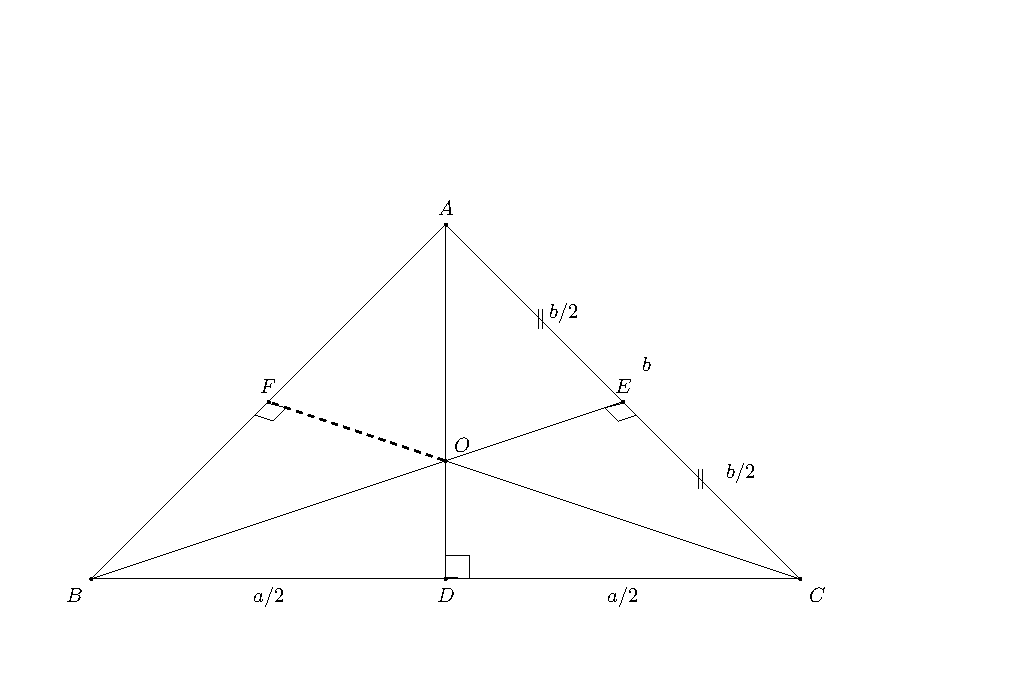
\includegraphics[width=\columnwidth]{./figs/fig_3.8.eps}
%%		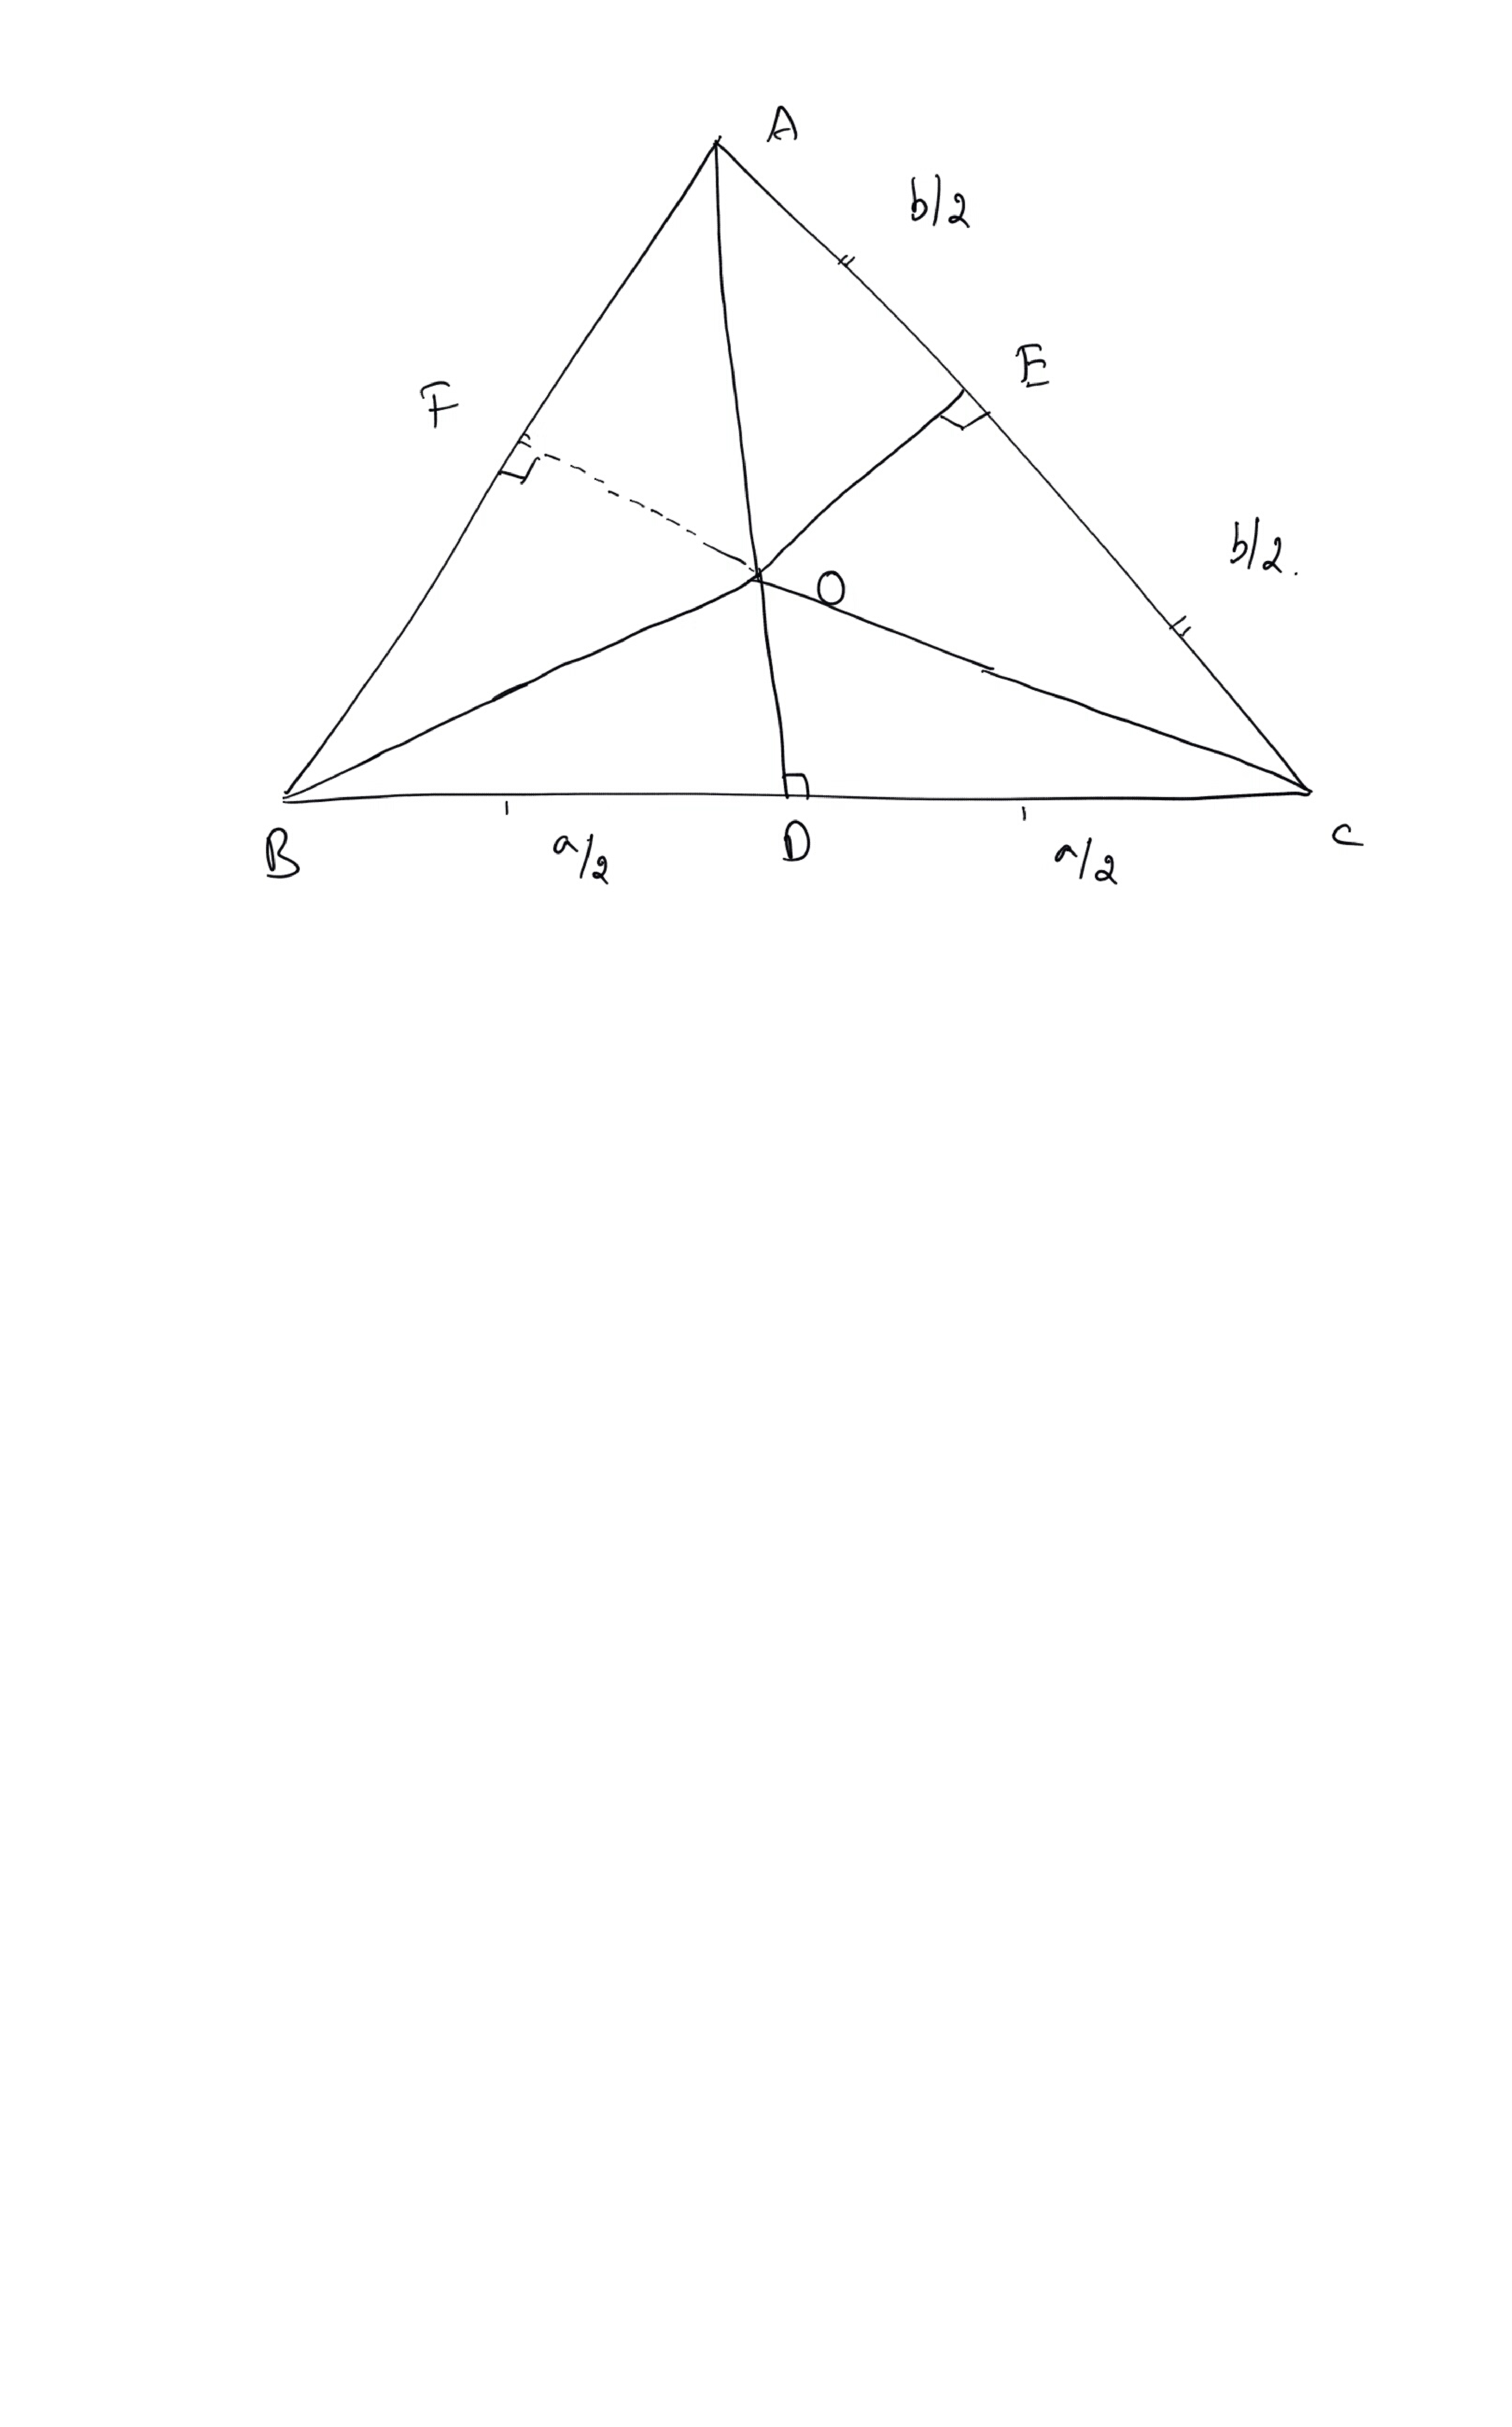
\includegraphics[width=\columnwidth]{./figs/ch3_perp_bisector}
%		%\vspace*{-10cm}
%%		\resizebox{\columnwidth}{!}{\documentclass{standalone}
\usepackage{tikz}
\usepackage{tkz-euclide}
\usetkzobj{all}
%\usepackage{amsmath}
\providecommand{\brak}[1]{\ensuremath{\left(#1\right)}}

\begin{document}
\begin{tikzpicture}
[scale=2,>=stealth,point/.style={draw,circle,fill = black,inner sep=0.5pt},]

\node (E) at (1.5, 1.5)[point,label=above :$E$] {};
\node (F) at (-1.5, 1.5)[point,label=above :$F$] {};
\node (A) at (0, 3)[point,label=above :$A$]{};
\node (B) at (-3, 0)[point,label=below left:$B$]{};
\node (C) at (3, 0)[point,label=below right:$C$]{};
\node (D) at (0,0)[point,label=below :$D$] {};
\node (O) at (0,1)[point,label=above right :$O$] {};


\draw (B)--(A);
\draw (A)--(C);
\draw (B)--(C);
\draw (B)--(E);
\draw (C)--(O);
\draw (A)--(D);
\draw [thick,dashed] (O) -- (F);

\node [above] at (1.7,1.7) {$b$};
\node [above] at (2.5,.75) {$b/2$};
\node [above] at (1,2.1) {$b/2$};
\node [above] at (-1.5,-0.3){$a/2$};
\node [above] at (1.5,-0.3){$a/2$};
\tkzMarkRightAngle[size=.16](B,F,O)
\tkzMarkRightAngle[size=.16](C,E,O)
\tkzMarkRightAngle[size=.2](A,D,C)
\draw   -- (4.3,1.7) node[midway] {$\parallel$};
\draw   -- (1.6,4.4) node[midway] {$\parallel$};

\end{tikzpicture}
\end{document}}
%	\end{center}
%	\caption{Perpendicular bisectors meet at a point}
%	\label{ch3_perp_bisector}	
%\end{figure}
%%
%\solution In $\Delta$s $ODB$ and $ODC$, using Budhayana's theorem,
%%
%\begin{equation}
%\begin{split}
%OB^2 &= OD^2 + BD^2 \\
%OC^2 &= OD^2 + DC^2 
%\end{split}
%\end{equation}
%%
%Since $BD = DC = \frac{a}{2}$, $OB = OC$.  Similarly, it can be shown that $OA = OC$.  Thus, $OA=OB=OC$.
%%
%\item
%	In $\Delta AOB$, $OA = OB$.  Such a triangle is known as an isoceles triangle.
%
%%
%\item
%	Show that $AF = BF$.
%
%\solution Trivial using Budhayana's theorem.  This shows that $OF$ is a perpendicular bisector of $AB$. 
%{\em Conclusion:}  The perpendicular bisectors of a triangle meet at a point.
%%
%\end{enumerate}
%
%\subsection{Perpendiculars from Vertex to Opposite Side}
%\renewcommand{\theequation}{\theenumi}
%\begin{enumerate}[label=\arabic*.,ref=\thesubsection.\theenumi]
%\numberwithin{equation}{enumi}
%	%
%	%
%\item
%	In Fig. \ref{ch3_perp_triang}, $AD \perp BC$ and $BE \perp AC$. $CF$ passes through $O$ and meets
%	$AB$ at $F$.  	
%	Show that 
%	\begin{align}
%	OE = c \cos A \cot C
%	\end{align}
%
%	\begin{figure}[!ht]
%		\begin{center}
%			
%			%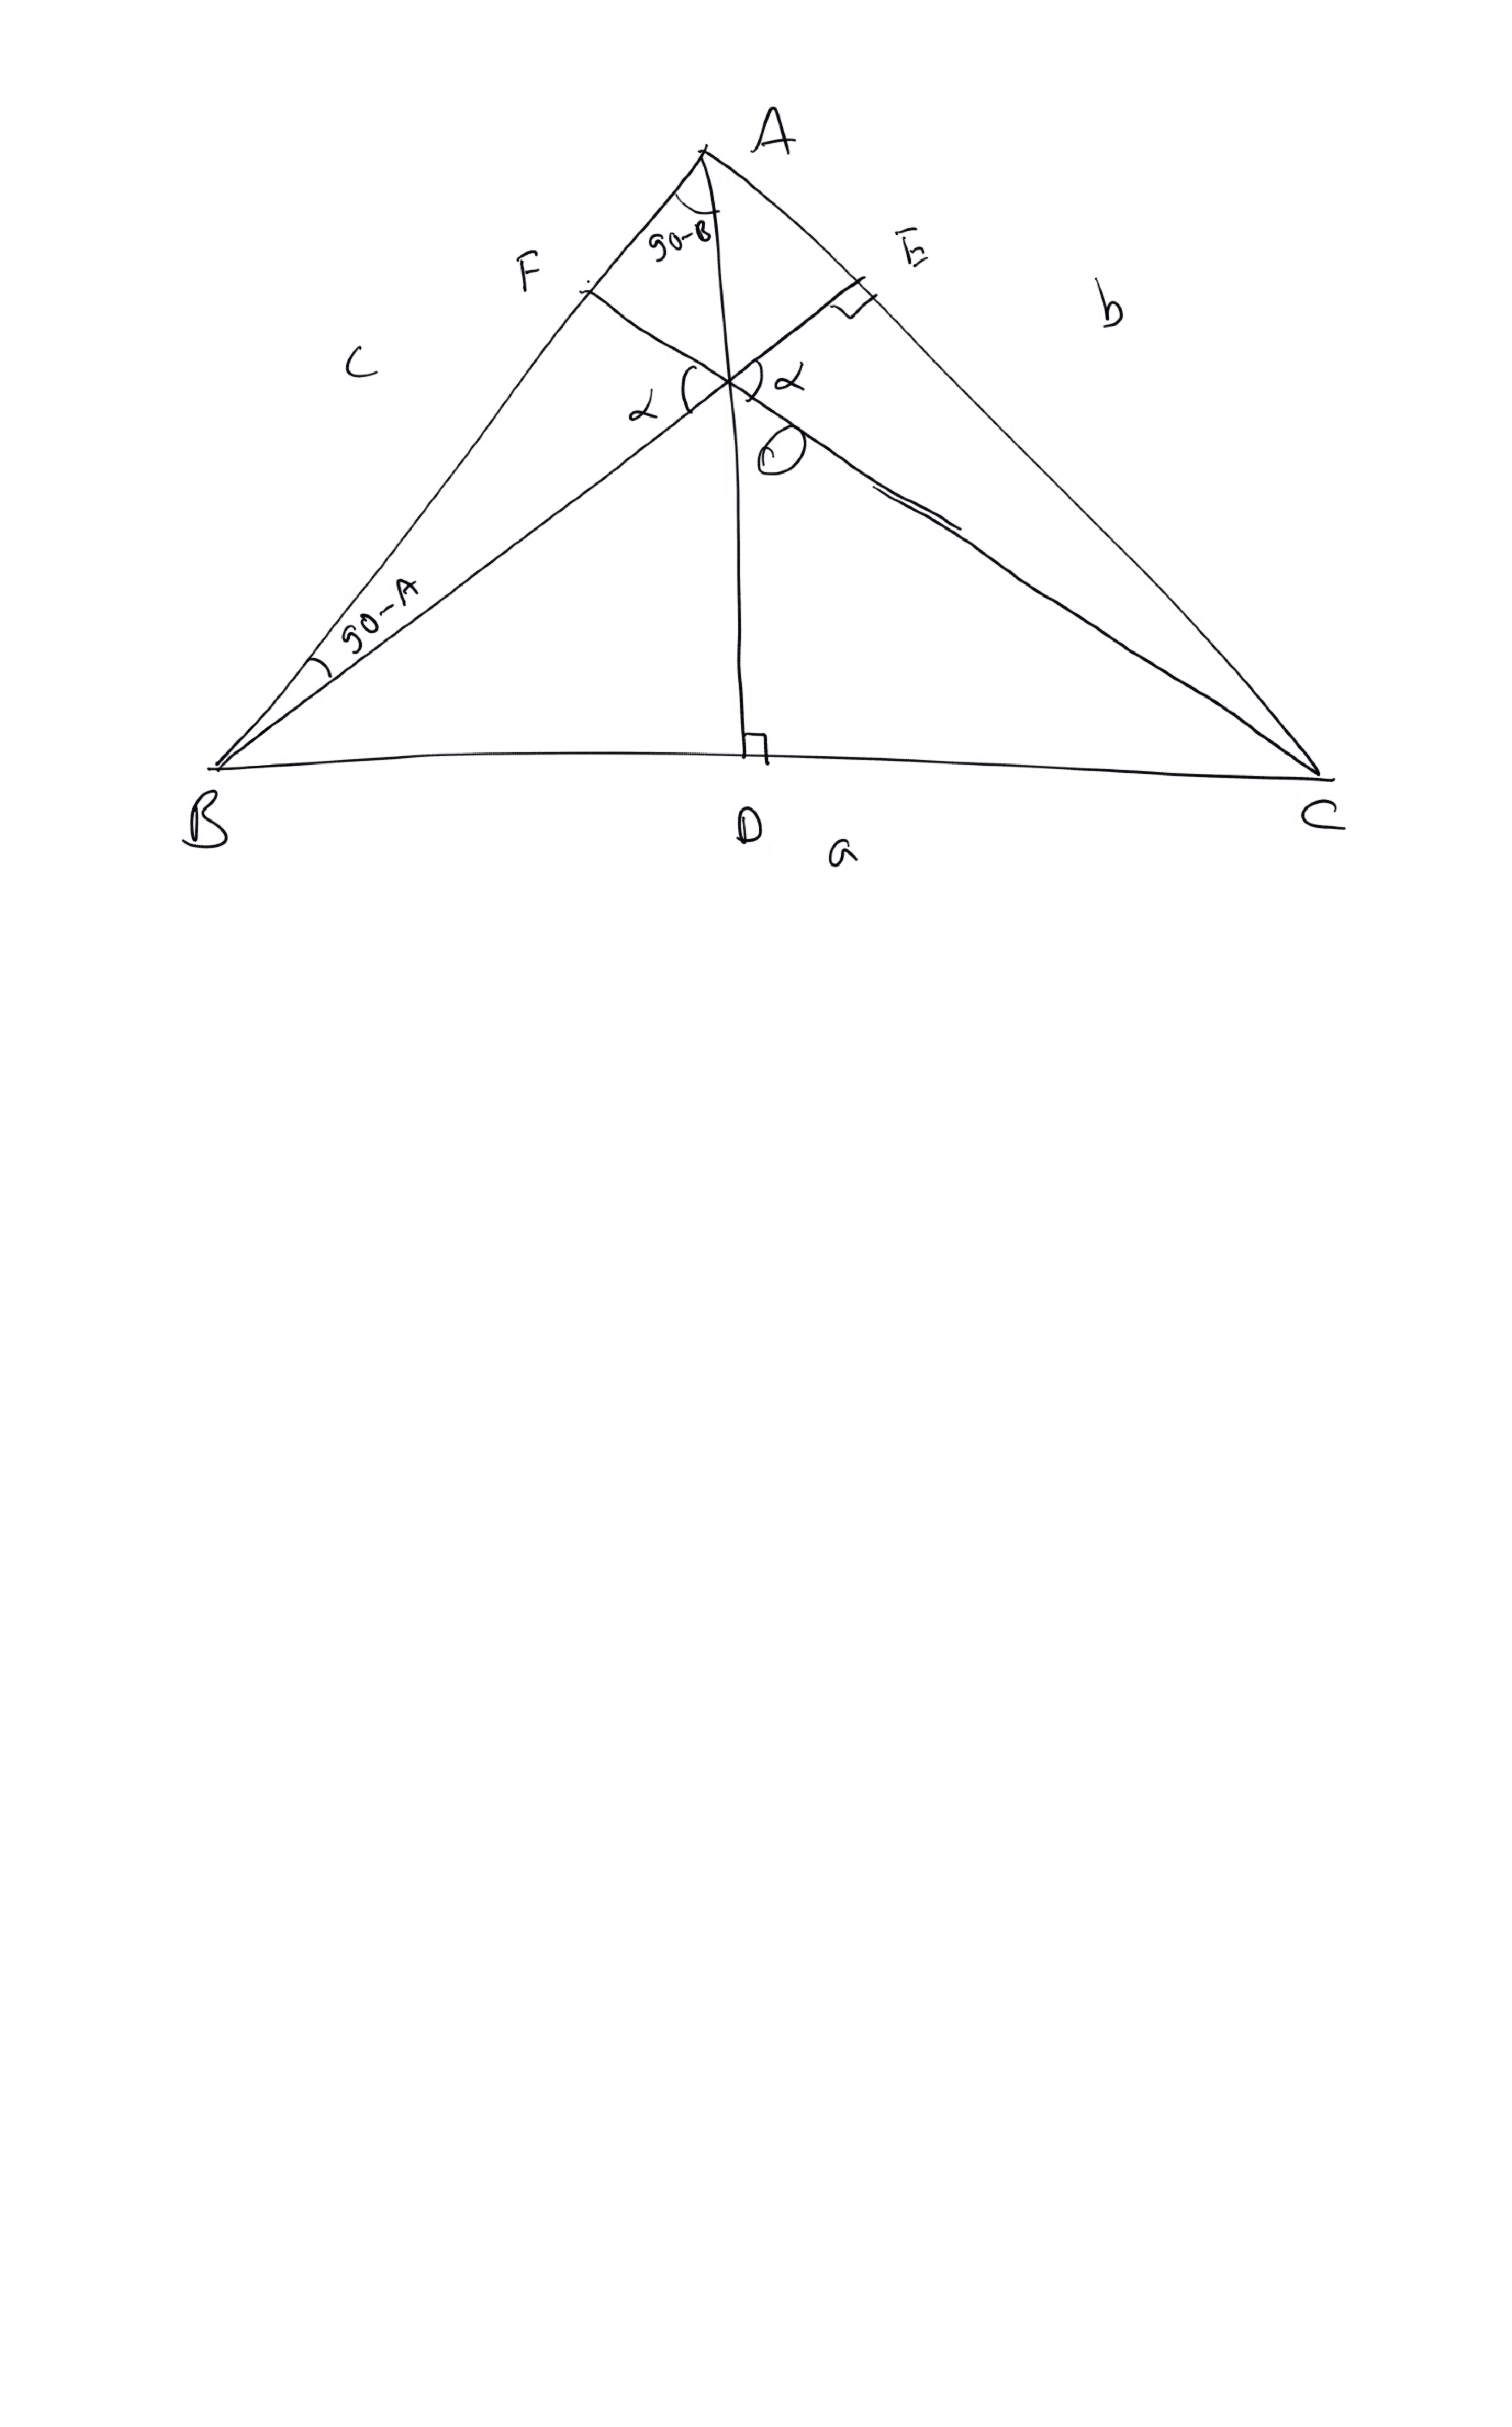
\includegraphics[width=\columnwidth]{./figs/ch3_perp_triang}
%			%\vspace*{-10cm}
%			\resizebox{\columnwidth}{!}{\begin{tikzpicture}
[scale=2,>=stealth,point/.style={draw,circle,fill = black,inner sep=0.5pt},]

\node (E) at (1.5, 1.5)[point,label=above :$E$] {};
\node (F) at (-1.5, 1.5)[point,label=above :$F$] {};
\node (A) at (0, 3)[point,label=above :$A$]{};
\node (B) at (-3, 0)[point,label=below left:$B$]{};
\node (C) at (3, 0)[point,label=below right:$C$]{};
\node (O) at (0,1)[point,label=above right :$O$] {};
\node (D) at (0,0)[point,label=below :$D$] {};


\draw (B)--(A);
\draw (A)--(C);
\draw (B)--(E);
\draw (C)--(F);
\draw (B)--(C);
\draw (A)--(D);

\node [below] at (0,-0.3) {$a$};
\node [above] at (-1.7,1.7) {$c$};
\node [above] at (1.7,1.7) {$b$};
\node [above] at (1,1.3) {$p$};
\node [above] at (-1,1.3) {$q$};
\node [above] at (-2.3,0.24){\rotatebox{45}{$90-A$}};
\node [above] at (-0.4,2.1) {\rotatebox{45}{$90-B$}};
\node [above] at (0.4,2.1) {\rotatebox{-45}{$90-C$}};

\tkzMarkAngle[size=.3](F,O,B);
\tkzMarkAngle[size=.3](C,O,E);
\tkzMarkAngle[size=.4](O,B,F);
\tkzMarkAngle[size=.2](F,A,O);
\tkzMarkAngle[size=.3](O,A,E);
\draw (-0.5,1) node{$\alpha$};
\draw (0.5,1) node{$\alpha$};

\end{tikzpicture}
}
%		\end{center}
%		\caption{Perpendiculars from vertex to opposite side meet at a point}
%		\label{ch3_perp_triang}	
%	\end{figure}
%%
%\solution In $\Delta$ s $AEB$ and $AEO$,
%%
%\begin{align}
%AE &= c \cos A \\
%OE &= AE \tan \brak{90^{\degree} - C} \brak{\because ADC \text{ is right angled}} \\
%&= AE \cot C
%\end{align}
%%
%From both the above, we get the desired result.
%%
%\item
%	Show that $\alpha = A$.
%
%\solution In $\Delta OEC$,
%%
%\begin{equation}
%CE = a \cos C \brak{\because BEC \text{ is right angled}}
%\end{equation}
%%
%Hence,
%%
%\begin{equation}
%\begin{split}
%\tan \alpha &= \frac{CE}{OE} \\
%&=  \frac{a \cos C}{c \cos A \cot C} \\
%&=  \frac{a \cos C \sin C}{c \cos A \cos C} \\
%&= \frac{a \sin C}{c \cos A } \\
%&= \frac{c \sin A}{c \cos A } \brak{\because \frac{a}{\sin A} = \frac{c}{\sin C}}\\
%&= \tan A\\
%\Rightarrow \alpha = A
%\end{split}
%\end{equation}
%%
%\item
%	Show that $CF \perp AB$
%
%\solution Consider triangle OFB and the result of the previous problem.  $\because$ the sum of the angles of a triangle is $180^{\degree}$, $\angle CFB = 90^{\degree}$.
%{\em Conclusion: The perperdiculars from the vertex of a triangle to the opposite side meet at a point.}
\end{enumerate}

%\newpage
%\newpage
\section{Quadrilaterals}
\subsection{Properties}
\renewcommand{\theequation}{\theenumi}
\begin{enumerate}[label=\arabic*.,ref=\thesubsection.\theenumi]
\numberwithin{equation}{enumi}
	%
\item In Fig. 	\ref{fig:tri_med_pgm}, 	$BDEF$ is defined as a {\em parallelogram}. Based on the properties of medians and similar triangles, we know that
\label{them:pgm_basic}
%
\begin{align}
BD &\parallel EF, BD = EF
\\
BF &\parallel DE, BF = DE
\\
OD &= OF, OB = OE
\end{align} 
Hence, 
\begin{enumerate}
\item opposite sides are equal 
\item  opposite angles are equal
\item  diagonals bisect each other
\item Adjacent angles of a paralleogram are supplementary.
\end{enumerate}
%
\begin{figure}[!ht]
	\begin{center}
		\resizebox{\columnwidth}{!}{%Code by GVV Sharma
%December 11, 2019
%released under GNU GPL
%Medians meet at a point

\begin{tikzpicture}
[scale=2,>=stealth,point/.style={draw,circle,fill = black,inner sep=0.5pt},]

%Triangle sides
\def\a{5}
\def\b{6}
\def\c{4}
 
%Coordinates of A
\def\p{2.25}
\def\q{{sqrt(\c^2-\p^2)}}

%Labeling points
\node (A) at (\p,\q)[point,label=above right:$A$] {};
\node (B) at (0, 0)[point,label=below left:$B$] {};
\node (C) at (\a, 0)[point,label=below right:$C$] {};

%Foot of median

\node (D) at ($(B)!0.5!(C)$)[point,label=below:$D$] {};
\node (E) at ($(A)!0.5!(C)$)[point,label=right:$E$] {};
\node (F) at ($(B)!0.5!(A)$)[point,label=left:$F$] {};

%Drawing triangle ABC
\draw (A) --  (B) -- (C) --  (A);

%Drawing medians AD, BE and CF
\draw (B) -- (E);
\draw (D) -- (F);
\node [above] at ($(F)!0.5!(D)$) {$O$};
%\draw (C) -- (F);
%\draw (A) -- (D);

%Drawing EF
\draw [dashed] (E) -- node[above] {$\frac{a}{2}$}(F);
\draw [dashed] (E) -- node[right] {$\frac{c}{2}$}(D);

%Centroid
%\node (G) at ($(B)!0.67!(E)$)[label={[shift={(0.8,-0.5)}]$G$}] {};

%Labeling sides
\node [right] at ($(A)!0.5!(E)$) {$\frac{b}{2}$};
\node [right] at ($(C)!0.5!(E)$) {$\frac{b}{2}$};
\node [left] at ($(B)!0.5!(F)$) {$\frac{c}{2}$};
\node [left] at ($(A)!0.5!(F)$) {$\frac{c}{2}$};
\node [below] at ($(B)!0.5!(D)$) {$\frac{a}{2}$};
\node [below] at ($(D)!0.5!(C)$) {$\frac{a}{2}$};
%\node [above] at ($(E)!0.5!(G)$) {$p$};
%\node [below] at ($(B)!0.5!(G)$) {$2p$};

%\node (G) at ($(B)!0.67!(E)$)[label={[shift={(-0.8,-0.5)}]$G_1$}] {};

%
\end{tikzpicture}

}
	\end{center}
	\caption{Parallelogram}
	\label{fig:tri_med_pgm}	
\end{figure}
%
\item In Fig. 	\ref{fig:tri_med_pgm}, $BFEC$ is a quadrilateral with $EF \parallel BC$ and is known as a {\em trapezium}.
\item Sum of the angles of a quadrilateral is 360$\degree$. 
\item Construct parallelogram $ABCD$ 	in Fig. \ref{fig:pgm_sas}	
given that  $BC = 5, AB = 6, \angle C = 85 \degree$.
\begin{figure}[!ht]
	\begin{center}
		\resizebox{\columnwidth}{!}{%Code by GVV Sharma
%December 10, 2019
%released under GNU GPL
%Drawing a parallelogram given 2 sides and a diagonal

\begin{tikzpicture}
[scale=2,>=stealth,point/.style={draw,circle,fill = black,inner sep=0.5pt},]

%Triangle sides
\def\a{5}
\def\b{6}
\def\c{7.467975323683154}
%Coordinates of A
%\def\p{{\a^2+\c^2-\b^2}/{(2*\a)}}
\def\p{4.477065543514051}
\def\q{{sqrt(\c^2-\p^2)}}

%Labeling points
\node (D) at (\p,\q)[point,label=above right:$D$] {};
\node (B) at (0, 0)[point,label=below left:$B$] {};
\node (C) at (\a, 0)[point,label=below right:$C$] {};
\node (O) at ($(B)!0.5!(D)$)[point,label=below right:$O$] {};

%Foot of perpendicular

\node (A) at ($(O)!-1!(C)$)[point,label=above right:$A$] {};


%Drawing parallelogram ABCD
\draw (A) -- (B) --  (C) --(D)--(A);
\draw (A) -- (C);
\draw (B) --(D);


\tkzMarkAngle[fill=green!20](C,A,D)
\tkzMarkAngle[fill=green!20](A,C,B)
%
%
\tkzMarkAngle[fill=red!30](A,D,B)
\tkzMarkAngle[fill=red!30](C,B,D)


\tkzMarkAngle[fill=orange!40](D,C,O)
\tkzMarkAngle[fill=orange!40](B,A,C)

\tkzMarkAngle[fill=blue!50](B,D,C)
\tkzMarkAngle[fill=blue!50](D,B,A)

\end{tikzpicture}
}
	\end{center}
	\caption{Parallelogram Properties}
	\label{fig:pgm_sas}	
\end{figure}
%
\\
\solution $BD$ is found using the cosine formula and $\triangle BDC$ is drawn using the approach in Construction \ref{const:tri_sss} with 
%
\begin{align}
\vec{B} = \myvec{0\\0},
\vec{C} = \myvec{5\\0},
\end{align}
%
Since the diagonals bisect each other, 
%
\begin{align}
\vec{O} &= \frac{\vec{B}+\vec{D}}{2}
\\
\vec{A} &= 2\vec{O} - \vec{C}.
\end{align}
%
$AB$ and $AD$ are then joined to complete the $\parallel$gm.
The python code for  Fig. \ref{fig:pgm_sas} is
\begin{lstlisting}
codes/quad/pgm_sas.py
\end{lstlisting}
%
and 
The equivalent latex-tikz code is
%
\begin{lstlisting}
figs/quad/pgm_sas.tex
\end{lstlisting}
%

\item A rectangle is a parallelogram with one right angle.
\item Draw the $\parallel$gm $ABCD$ in 	Fig. \ref{fig:pgm_sss}	
with $BC = 6, CD = 4.5$ and $BD=7.5$.  Show that it is a rectangle.
\label{const:pgm_sss}
%
\begin{figure}[!ht]
	\begin{center}
		\resizebox{\columnwidth}{!}{%Code by GVV Sharma
%December 10, 2019
%released under GNU GPL
%Drawing a parallelogram given 2 sides and a diagonal

\begin{tikzpicture}
[scale=2,>=stealth,point/.style={draw,circle,fill = black,inner sep=0.5pt},]

%Triangle sides
\def\a{6}
\def\b{4.5}
\def\c{7.5}
%Coordinates of A
%\def\p{{\a^2+\c^2-\b^2}/{(2*\a)}}
\def\p{6}
\def\q{{sqrt(\c^2-\p^2)}}

%Labeling points
\node (D) at (\p,\q)[point,label=above right:$D$] {};
\node (B) at (0, 0)[point,label=below left:$B$] {};
\node (C) at (\a, 0)[point,label=below right:$C$] {};
\node (O) at ($(B)!0.5!(D)$)[point,label=below right:$O$] {};

%Foot of perpendicular

\node (A) at ($(O)!-1!(C)$)[point,label=above right:$A$] {};


%Drawing parallelogram ABCD
\draw (A) -- (B) --  (C) --(D)--(A);
\draw (A) -- (C);
\draw (B) --(D);


%\tkzMarkAngle[fill=green!20](C,A,D)
%\tkzMarkAngle[fill=green!20](A,C,B)
%%
%%
%\tkzMarkAngle[fill=red!30](A,D,B)
%\tkzMarkAngle[fill=red!30](C,B,D)
%
%
%\tkzMarkAngle[fill=orange!40](D,C,O)
%\tkzMarkAngle[fill=orange!40](B,A,C)
%
%\tkzMarkAngle[fill=blue!50](B,D,C)
%\tkzMarkAngle[fill=blue!50](D,B,A)
%
\end{tikzpicture}
}
	\end{center}
	\caption{Rectangle}
	\label{fig:pgm_sss}	
\end{figure}
\\
\solution It is easy to verify that 
%Using the approach in Construction\ref{const:tri_sss}, $\triangle BCD$ is drawn with
%
\begin{align}
BD^2=BC^2+C^2
\end{align}
%
Hence, using Baudhayana theorem, 
%
\begin{align}
\angle BCD = 90\degree
\end{align}
%
and  $ABCD$ is a rectangle.
\begin{align}
\vec{A} = \myvec{0\\4.5}
\vec{B} = \myvec{0\\0}
\vec{C} = \myvec{6\\0}
\vec{D} = \myvec{6\\4}
\end{align}
%
The python code for  Fig. \ref{fig:pgm_sss} is
\begin{lstlisting}
codes/quad/pgm_sss.py
\end{lstlisting}
%
and the equivalent latex-tikz code is
%
\begin{lstlisting}
figs/quad/pgm_sss.tex
\end{lstlisting}
%
\item  Diagonals of a rectangle are equal and vice-versa. 
\\
\solution Follows from the fact that $\triangle BCD \cong \triangle ABC$. 
%
\item A rhombus, shown in Fig. 	\ref{fig:rhom_sss}	
 is a parallelogram with equal sides.  
%
\begin{figure}[!ht]
	\begin{center}
		\resizebox{\columnwidth}{!}{%Code by GVV Sharma
%December 10, 2019
%released under GNU GPL
%Drawing a rhombus given a side and a diagonal

\begin{tikzpicture}
[scale=2,>=stealth,point/.style={draw,circle,fill = black,inner sep=0.5pt},]

%Triangle sides
\def\a{4.5}%BE
\def\b{6}%ET
\def\p{\b/2}%OE
\def\q{{sqrt(\a^2-\p^2)}}%OB

%Labeling points
\node (B) at (0,-\q)[point,label=below :$B$] {};
\node (E) at (\p, 0)[point,label=right:$E$] {};
\node (S) at (0, \q)[point,label=above:$S$] {};
\node (T) at (-\p,0)[point,label=left:$T$] {};
\node (O) at (0, 0)[point,label=below left:$O$] {};


%Drawing parallelogram ABCD
\draw (B) -- (E) --  (S) --(T)--(B);
\draw (B) -- (S);
\draw (E) --(T);


\tkzMarkRightAngle[fill=blue!20,size=.2](B,O,E)

%
\end{tikzpicture}
}
	\end{center}
	\caption{Rhombus}
	\label{fig:rhom_sss}	
\end{figure}
%
\item Diagonals of a rhombus bisect each other at right angles.
\\
\solution 	In Fig. \ref{fig:rhom_sss}, 	from Theorem \ref{them:pgm_basic}, $OB = OS$.
From Theorem \ref{them:isos_pb}, $OE \perp BS$.
%
\item Draw the rhombus $BEST$ with $BE = 4.5$ and $ET = 6$. 
\\
\solution The coordinates of the various points in Fig. \ref{fig:rhom_sss} are obtained as
%
\begin{align}
\vec{O} = \myvec{0\\0},
\vec{B} = \myvec{0\\-4.5}
\\
\vec{E} = \myvec{3\\0},
\vec{S} = \myvec{4.5\\0},
\vec{T} = \myvec{0\\-3}
\end{align}
%
\item A square is a rectangle whose sides are equal.  Draw a square of side 4.5.
\\
\solution The coordinates of the various points in Fig. \ref{fig:square} are obtained as
%
\begin{align}
\vec{A} = \myvec{0\\4.5}
\\
\vec{B} = \myvec{0\\0},
\vec{C} = \myvec{4.5\\0},
\vec{D} = \myvec{4.5\\4.5}
\vec{O} = \frac{\vec{B}+\vec{C}}{2}
%
\end{align}
%
\begin{figure}[!ht]
	\begin{center}
		\resizebox{\columnwidth}{!}{%Code by GVV Sharma
%December 12, 2019
%released under GNU GPL
%Drawing a square given a side 

\begin{tikzpicture}
[scale=2,>=stealth,point/.style={draw,circle,fill = black,inner sep=0.5pt},]

%Square side
\def\a{4.5}

%Labeling points
\node (A) at (0,\a)[point,label=below :$A$] {};
\node (B) at (0,0)[point,label=below :$B$] {};
\node (C) at (\a, 0)[point,label=right:$C$] {};
\node (D) at (\a, \a)[point,label=above:$D$] {};
\node (O) at ($(B)!0.5!(D)$)[point,label=below left:$O$] {};


%Drawing square ABCD
\draw (A) -- (B) --  (C) --(D)--(A);
\draw (B) -- (D);
\draw (A) --(C);


\tkzMarkRightAngle[fill=blue!20,size=.2](C,O,D)
\tkzMarkRightAngle[fill=blue!20,size=.2](A,B,C)

%
\end{tikzpicture}
}
	\end{center}
	\caption{Square}
	\label{fig:square}	
\end{figure}

\item  Diagonals of a square bisect each other at right angles and are equal, and vice-versa. 
%
\\
\solution A square has the properties of a rectangle as well as a rhombus.
%
%
\item Area of a parallelogram is the product of its base and the corresponding altitude. 
%
\end{enumerate}


\section{Circle}
%\subsection{Properties}
\subsection{Properties}
%
\renewcommand{\theequation}{\theenumi}
\begin{enumerate}[label=\arabic*.,ref=\thesubsection.\theenumi]
\numberwithin{equation}{enumi}
%
\item
	Fig. \ref{ch4_circle_def} represents a circle, which passes through the vertices $A B, C$ of  $\triangle ABC$ in Fig.  	\eqref{ch3_perp_bisector}	
 The points in the circle are at a distance $R$ from the {\em centre} $O$.  $R$ is known as the {\em radius}. The line  joining any two points on a circle is known as a {\em chord}.  Thus, the sides of $\triangle ABC$ are chords.

\begin{figure}[!ht]
	\begin{center}
		
		%
\includegraphics[width=\columnwidth]{./figs/ch4_circle_def}
		%\vspace*{-10cm}
%		\resizebox{\columnwidth}{!}{\begin{tikzpicture}
[
scale =3,
>=stealth,
point/.style = {draw, circle, fill = black, inner sep = 1pt},
]
\def\rad{1}
\coordinate [point, label={above : $O$ }] (O) at (0, 0);
\draw (O) circle (\rad);
\node (A) at (-0.7,-0.7)[point,label=above :$A$] {};
\node (B) at (0.7,-0.7)[point,label=above :$B$] {};

\draw (A)--(O);
\draw (O)--(B);
\draw (B)--(A);

\node [above] at (-0.4,-0.4) {$r$};
\node [above] at (0.4,-0.4) {$r$};

\end{tikzpicture}
}
		\resizebox{\columnwidth}{!}{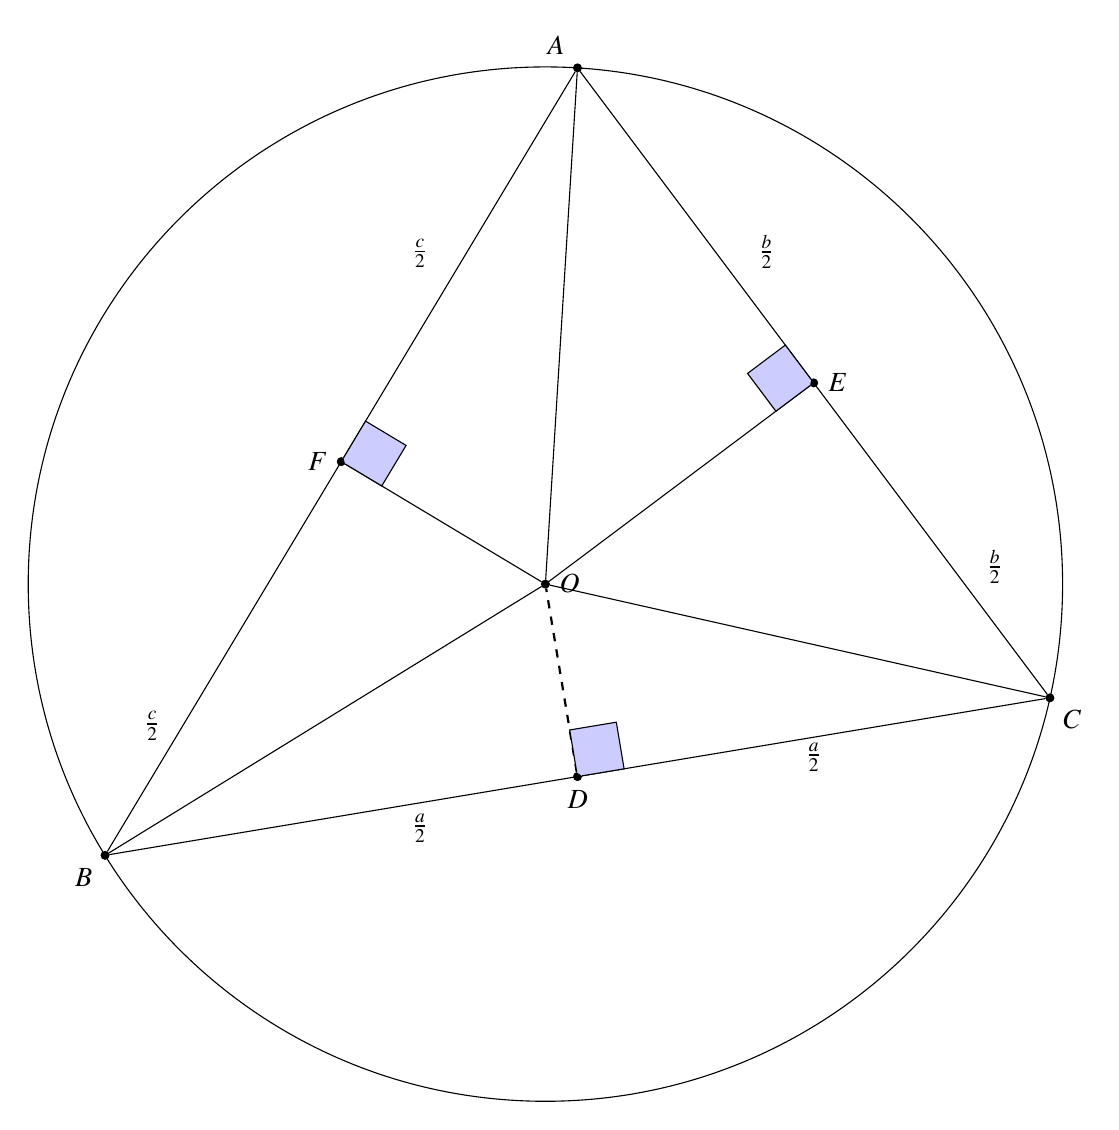
\begin{tikzpicture}
[
 scale=2,
  >=stealth,
  point/.style = {draw, circle, fill = black, inner sep = 1pt},
]
\node (B) at (-2,-2)[point,label = below left:${B}$] {};
\node (A) at (1,3)[point,label = above left:${A}$] {};
\node (C) at (4,-1)[point,label = below right:${C}$] {};
\draw (A) -- (B) -- (C) -- (A);

\node (D) at (1,-1.5)[point,label = below:$D$] {};

\node (F) at (-0.5,0.5)[point,label = left:$F$] {};

\node (E) at (2.5,1)[point,label = right:$E$] {};

\node (O) at (0.7962963,-0.27777778) [point,label = right:$O$] {};

\draw[thick, dashed] (D) -- (O);
\draw (F) -- (O);
\draw (E) -- (O);
\draw (A) -- (O);
\draw (B) -- (O);
\draw (C) -- (O);

\tkzMarkRightAngle[fill=blue!20,size=.3](A,E,O)
\tkzMarkRightAngle[fill=blue!20,size=.3](A,F,O)
\tkzMarkRightAngle[fill=blue!20,size=.3](O,D,C)


\node [below] at (3.65,0) {\strut $\frac{b}{2}$};
\node [below] at (2.2,2) {\strut  $\frac{b}{2}$};


\node [below] at (2.5,-1.2) {\strut  $\frac{a}{2}$};    
\node [below] at (0,-1.65) {\strut  $\frac{a}{2}$};  
      
\node [below] at (-1.7,-1) {\strut  $\frac{c}{2}$}; 
\node [below] at (0,2) {\strut  $\frac{c}{2}$};   

\def\rad{3.284101453883}
%\coordinate [point, label={above : $O$ }] (O) at (0, 0);
\draw (O) circle (\rad);

\end{tikzpicture}
}
%		\resizebox{\columnwidth}{!}{\begin{tikzpicture}
[
scale =3,
>=stealth,
point/.style = {draw, circle, fill = black, inner sep = 1pt},
]
\def\rad{1}
\coordinate [point, label={above : $O$ }] (O) at (0, 0);
\draw (O) circle (\rad);
\node (A) at (-0.7,-0.7)[point,label=above :$A$] {};
\node (B) at (0.7,-0.7)[point,label=above :$B$] {};

\draw (A)--(O);
\draw (O)--(B);
\draw (B)--(A);

\node [above] at (-0.4,-0.4) {$r$};
\node [above] at (0.4,-0.4) {$r$};

\end{tikzpicture}
}
	\end{center}
	\caption{Circle Definitions}
	\label{ch4_circle_def}	
\end{figure}
%\item
%	In Fig. \ref{ch4_circle_def}, $A$ and $B$ are points on the circle.  The line $AB$ is known as a chord of the circle.

%
%
%\item
%	\label{ch4_prob_circle_subtend}
%	In Fig. \ref{ch4_circle_subtend}  
%%Show that $\angle AOB = 2\angle ACB $.
%
%\begin{figure}[!ht]
%	\begin{center}
%		
%		%
\includegraphics[width=\columnwidth]{./figs/ch4_circle_subtend}
%		%\vspace*{-10cm}
%		\resizebox{\columnwidth}{!}{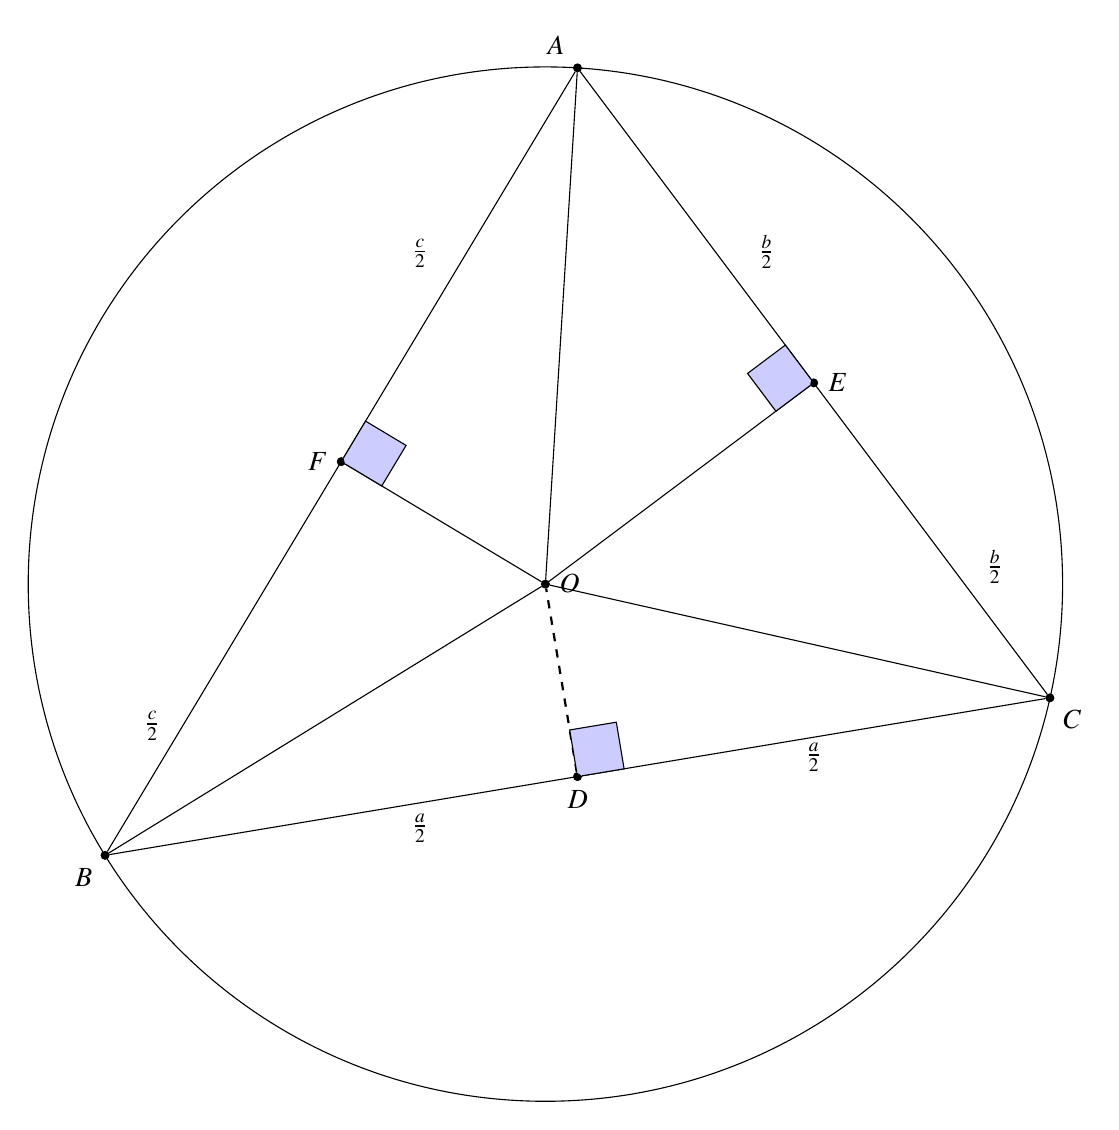
\begin{tikzpicture}
[
 scale=2,
  >=stealth,
  point/.style = {draw, circle, fill = black, inner sep = 1pt},
]
\node (B) at (-2,-2)[point,label = below left:${B}$] {};
\node (A) at (1,3)[point,label = above left:${A}$] {};
\node (C) at (4,-1)[point,label = below right:${C}$] {};
\draw (A) -- (B) -- (C) -- (A);

\node (D) at (1,-1.5)[point,label = below:$D$] {};

\node (F) at (-0.5,0.5)[point,label = left:$F$] {};

\node (E) at (2.5,1)[point,label = right:$E$] {};

\node (O) at (0.7962963,-0.27777778) [point,label = right:$O$] {};

\draw[thick, dashed] (D) -- (O);
\draw (F) -- (O);
\draw (E) -- (O);
\draw (A) -- (O);
\draw (B) -- (O);
\draw (C) -- (O);

\tkzMarkRightAngle[fill=blue!20,size=.3](A,E,O)
\tkzMarkRightAngle[fill=blue!20,size=.3](A,F,O)
\tkzMarkRightAngle[fill=blue!20,size=.3](O,D,C)


\node [below] at (3.65,0) {\strut $\frac{b}{2}$};
\node [below] at (2.2,2) {\strut  $\frac{b}{2}$};


\node [below] at (2.5,-1.2) {\strut  $\frac{a}{2}$};    
\node [below] at (0,-1.65) {\strut  $\frac{a}{2}$};  
      
\node [below] at (-1.7,-1) {\strut  $\frac{c}{2}$}; 
\node [below] at (0,2) {\strut  $\frac{c}{2}$};   

\def\rad{3.284101453883}
%\coordinate [point, label={above : $O$ }] (O) at (0, 0);
\draw (O) circle (\rad);

\end{tikzpicture}
}
%%		\resizebox{\columnwidth}{!}{\begin{tikzpicture}
[scale =2,>=stealth,point/.style = {draw, circle, fill = black, inner sep = 1pt},]

\def\rad{3}
\coordinate [point, label={above right: $O$ }] (O) at (0, 0);
\draw (O) circle (\rad);
\node (A) at (-2.24,-2)[point,label=below left :$A$] {};
\node (B) at (2.24,-2)[point,label=below right :$B$] {};
\node (C) at (0,3)[point,label=above :$C$] {};
\node (D) at (0,-2)[point,label=below :$D$] {};

\draw (A)--(B);
\draw (B)--(C);
\draw (C)--(A);
\draw (O)--(A);
\draw (O)--(B);
\draw [thick,dashed] (C)--(D);
\tkzMarkAngle[size=0.5](A,C,O)
\tkzMarkAngle[size=0.56](O,C,B)
\tkzMarkAngle[size=0.3](A,O,D)
\tkzMarkAngle[size=0.36](D,O,B)

\draw (-0.1,2.4) node{$\theta_1$};
\draw (0.15,2.3) node{$\theta_2$};

\node [above] at (-0.1,1){$r$};
\node [above] at (-1.1,-1){$r$};
\node [above] at (1.12,-1){$r$};
\node [above] at (-0.2,-0.5){$\alpha$};
\node [above] at (0.2,-0.6){$\beta$};

\end{tikzpicture}
}
%	\end{center}
%	\caption{Angle subtended by chord $AB$ at the centre $O$ is twice the angle subtended at $P$. }
%	\label{ch4_circle_subtend}	
%\end{figure}

%\solution In Fig. \ref{ch4_circle_subtend}, the triangleles $OPA$ and $OPB$ are isosceles. Hence,
%%
%\begin{align}
%\angle OCA = \angle OAC &= \theta_1 \\
%\angle OCB = \angle OBC &= \theta_2
%\end{align}
%%
%Also, $\alpha$ and $\beta$ are exterior angles corresponding to the triangle $AOC$ and $BOC$ respectively. Hence
%%
%\begin{align}
%\alpha &= 2\theta_1 \\
%\beta &= 2\theta_2
%\end{align}
%%
%Thus,
%%
%\begin{align}
%\angle AOB &= \alpha + \beta \\
%&= 2\brak{\theta_1 + \theta_2} \\
%&= 2\angle ACB
%\end{align}
%
\item
	The diameter of a circle is the chord that divides the circle into two equal parts. In Fig. \ref{ch4_circle_dia}, $AB$ is the diameter and passes through the centre $O$

%
\item
In Fig. \ref{ch4_circle_dia}, show that $\angle APB = 90^{\degree}$ .

%
\begin{figure}[!ht]
	\begin{center}
		
		%
\includegraphics[width=\columnwidth]{./figs/ch4_circle_dia}
		%\vspace*{-10cm}
		\resizebox{\columnwidth}{!}{\begin{tikzpicture}
[scale =3,>=stealth,point/.style = {draw, circle, fill = black, inner sep = 1pt},]

\def\rad{2}
\coordinate [point, label={above : $O$ }] (O) at (0, 0);
\draw (O) circle (\rad);
\node (A) at (-2,0)[point,label=above left :$A$] {};
\node (B) at (2,0)[point,label=above right :$B$] {};
\node (P) at (0,2)[point,label=above :$P$] {};


\draw (A)--(B);
\draw (P)--(A);
\draw (P)--(B);

\tkzMarkRightAngle[size=.2](B,P,A)

\end{tikzpicture}}
	\end{center}
	\caption{Diameter of a circle.}
	\label{ch4_circle_dia}	
\end{figure}
\item
	In Fig. \ref{ch4_chord_product}, show that 
	\begin{equation}
	\begin{split}
\angle ABD &= \angle ACD \\
\angle CAB &= \angle CDB	
	\end{split}
	\end{equation}

\begin{figure}[!ht]
	\begin{center}
		
		%
\includegraphics[width=\columnwidth]{./figs/ch4_chord_product}
		%\vspace*{-10cm}
		\resizebox{\columnwidth}{!}{\begin{tikzpicture}
[scale =2,>=stealth,point/.style = {draw, circle, fill = black, inner sep = 1pt},]

\def\rad{3}
\coordinate [point, label={right: $P$ }] (P) at (0, 0);
\draw (P) circle (\rad);
\node (A) at (-2.24,-2)[point,label=below left :$A$] {};
\node (C) at (2.24,-2)[point,label=below right :$C$] {};
\node (B) at (2.24,2)[point,label=above :$B$] {};
\node (D) at (-2.24,2)[point,label=below :$D$] {};

\draw (A)--(B);
\draw (C)--(D);
\draw [thick,dashed] (A)--(C);
\draw [thick,dashed] (B)--(D);
\tkzMarkAngle[size=0.3](P,D,B)
\tkzMarkAngle[size=0.3](D,B,P)
\tkzMarkAngle[size=0.3](B,P,D)
\tkzMarkAngle[size=0.3](A,P,C)
\tkzMarkAngle[size=0.3](C,A,P)
\tkzMarkAngle[size=0.3](P,C,A)

\draw (1.8,1.8) node{$\alpha$};
\draw (-1.84,1.84) node{$\beta$};
\draw (-1.8,-1.9) node{$\beta$};
\draw (1.8,-1.9) node{$\alpha$};
\draw (0,0.4) node{$\theta$};
\draw (0,-0.4) node{$\theta$};

\end{tikzpicture}}
	\end{center}
	\caption{$PA.PB = PC.PD$}
	\label{ch4_chord_product}	
\end{figure}
%
%
\solution Use Problem \ref{ch4_prob_circle_subtend}.
%
\item
	In Fig. \ref{ch4_chord_product}, show that the triangles $PAB$ and $PBD$ are similar

\solution Trivial using previous problem
\item
	In Fig. \ref{ch4_chord_product}, show that 
	\begin{equation}
	PA.PB = PC.PD
	\end{equation}

%
\solution Since triangles $PAC$ and $PBD$ are similar, 
%
\begin{align}
\frac{PA}{PD} &= \frac{PC}{PB} \\
\Rightarrow PA.PB &= PC.PD
\end{align}
%
\item
	Fig. \ref{fig:incirc_def} touches the sides of $\triangle ABC$ \eqref{ch3_angle_bisector} and is known as  the {\em incircle}.  The sides of the $\triangle$	are known as the {\em tangents} of the circle.

\begin{figure}[!ht]
	\begin{center}
		
		%
\includegraphics[width=\columnwidth]{./figs/ch4_circle_def}
		%\vspace*{-10cm}
%		\resizebox{\columnwidth}{!}{\begin{tikzpicture}
[
scale =3,
>=stealth,
point/.style = {draw, circle, fill = black, inner sep = 1pt},
]
\def\rad{1}
\coordinate [point, label={above : $O$ }] (O) at (0, 0);
\draw (O) circle (\rad);
\node (A) at (-0.7,-0.7)[point,label=above :$A$] {};
\node (B) at (0.7,-0.7)[point,label=above :$B$] {};

\draw (A)--(O);
\draw (O)--(B);
\draw (B)--(A);

\node [above] at (-0.4,-0.4) {$r$};
\node [above] at (0.4,-0.4) {$r$};

\end{tikzpicture}
}
		\resizebox{\columnwidth}{!}{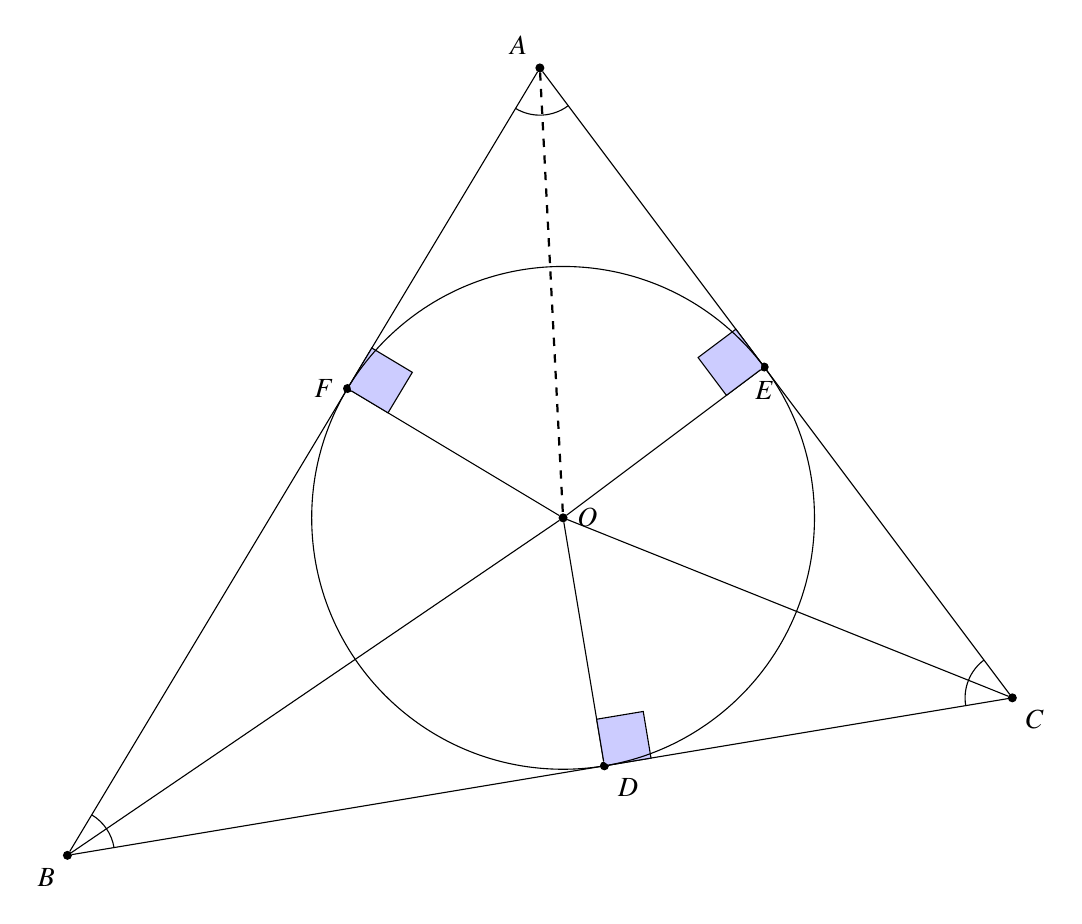
\begin{tikzpicture}
[
 scale=2,
  >=stealth,
  point/.style = {draw, circle, fill = black, inner sep = 1pt},
]

\node (B) at (-2,-2)[point,label = below left:${B}$] {};
\node (A) at (1,3)[point,label = above left:${A}$] {};
\node (C) at (4,-1)[point,label = below right:${C}$] {};
\draw (A) -- (B) -- (C) -- (A);
\node (O) at (1.14738665, 0.14292163) [point,label = right:$O$] {};

\node (D) at (1.40982295, -1.43169617)[point,label = below right:$D$] {};
\draw (O) -- (D);

\node (E) at (2.42445681, 1.10072425)[point,label = below:$E$] {};
\draw (O) -- (E);
%\draw[thick, dashed] (A) -- (E);


\node (F) at (-0.22146164,  0.9642306)[point,label = left:$F$] {};
\draw (O) -- (F);
\draw (O) -- (C);
\draw (O) -- (B);
\draw[thick, dashed] (A) -- (O);
%\draw (O) -- (A);


\tkzMarkAngle[fill=blue!60,size=.3](O,B,F)
\tkzMarkAngle[fill=blue!40,size=.3](D,B,O)


\tkzMarkAngle[fill=red!60,size=.3](F,A,O)
\tkzMarkAngle[fill=red!40,size=.3](O,A,E)


\tkzMarkAngle[fill=orange!60,size=.3](E,C,O)
\tkzMarkAngle[fill=orange!40,size=.3](O,C,D)

\tkzMarkRightAngle[fill=blue!20,size=.3](A,E,O)
\tkzMarkRightAngle[fill=blue!20,size=.3](A,F,O)
\tkzMarkRightAngle[fill=blue!20,size=.3](O,D,C)

\def\rad{1.596337700952456}
%%\coordinate [point, label={above : $O$ }] (O) at (0, 0);
\draw (O) circle (\rad);

\end{tikzpicture}
}
%		\resizebox{\columnwidth}{!}{\begin{tikzpicture}
[
scale =3,
>=stealth,
point/.style = {draw, circle, fill = black, inner sep = 1pt},
]
\def\rad{1}
\coordinate [point, label={above : $O$ }] (O) at (0, 0);
\draw (O) circle (\rad);
\node (A) at (-0.7,-0.7)[point,label=above :$A$] {};
\node (B) at (0.7,-0.7)[point,label=above :$B$] {};

\draw (A)--(O);
\draw (O)--(B);
\draw (B)--(A);

\node [above] at (-0.4,-0.4) {$r$};
\node [above] at (0.4,-0.4) {$r$};

\end{tikzpicture}
}
	\end{center}
	\caption{Incircle and Tangent}
	\label{fig:incirc_def}	
\end{figure}
%
\item Tangents to a circle from any point outside the circle are equal.
\\
\solution See Fig. \ref{fig:incirc_def} and use \eqref{eq:tang_eq}.

\item
	Show that 
	\begin{equation}
	\label{ch5_sin_90}
	\sin 90^{\degree} = 1
	\end{equation}
\solution From 	Prolem \ref{prob:ch2_triang_area}
and Problem \ref{prob:tri_area_sin}, the area of the right angled $\triangle ABC$ in Fig. \ref{ch2_sq_ar} is 	
	\begin{equation}
	\label{ch5_sin_90_der}
	\frac{1}{2}ab = \frac{1}{2}ab\sin 90^{\degree} 
	\end{equation}
%
resulting in 	\eqref{ch5_sin_90}.
\item
	Show that 
	\begin{equation}
	\label{ch5_cos_90}
	\cos 90^{\degree} = 0
	\end{equation}

\solution 
Follows from the fact that $\sin 90\degree = 1$ and \eqref{eq:tri_sin_cos_id}.



%
% 	
\item
	The line $PX$ in Fig. \ref{ch4_tangent_def} touches the circle at exactly one  point $P$. 
%It is known as the tangent to the circle.
%
%
	Show that $OP \perp PX$.
% is the perpendicular to the line $PX$ as shown in the Fig. \ref{ch4_short_dist}. Show that $OP$ is the shortest distance between the point $O$ and the line $PX$. 

\solution Without loss of generality, let $0 \le \theta \le 90^{\degree}$. Using the cosine formula in $\triangle OPP_n$,\begin{align}
\brak{r+d_n}^2 > r^2,
\end{align}
%Let $P_1$ be a point on the line $PX$. Then $OPP_1$ is a right angled triangle.  Using Budhayana's theorem,
%
\begin{figure}[!ht]
	\begin{center}
		
		%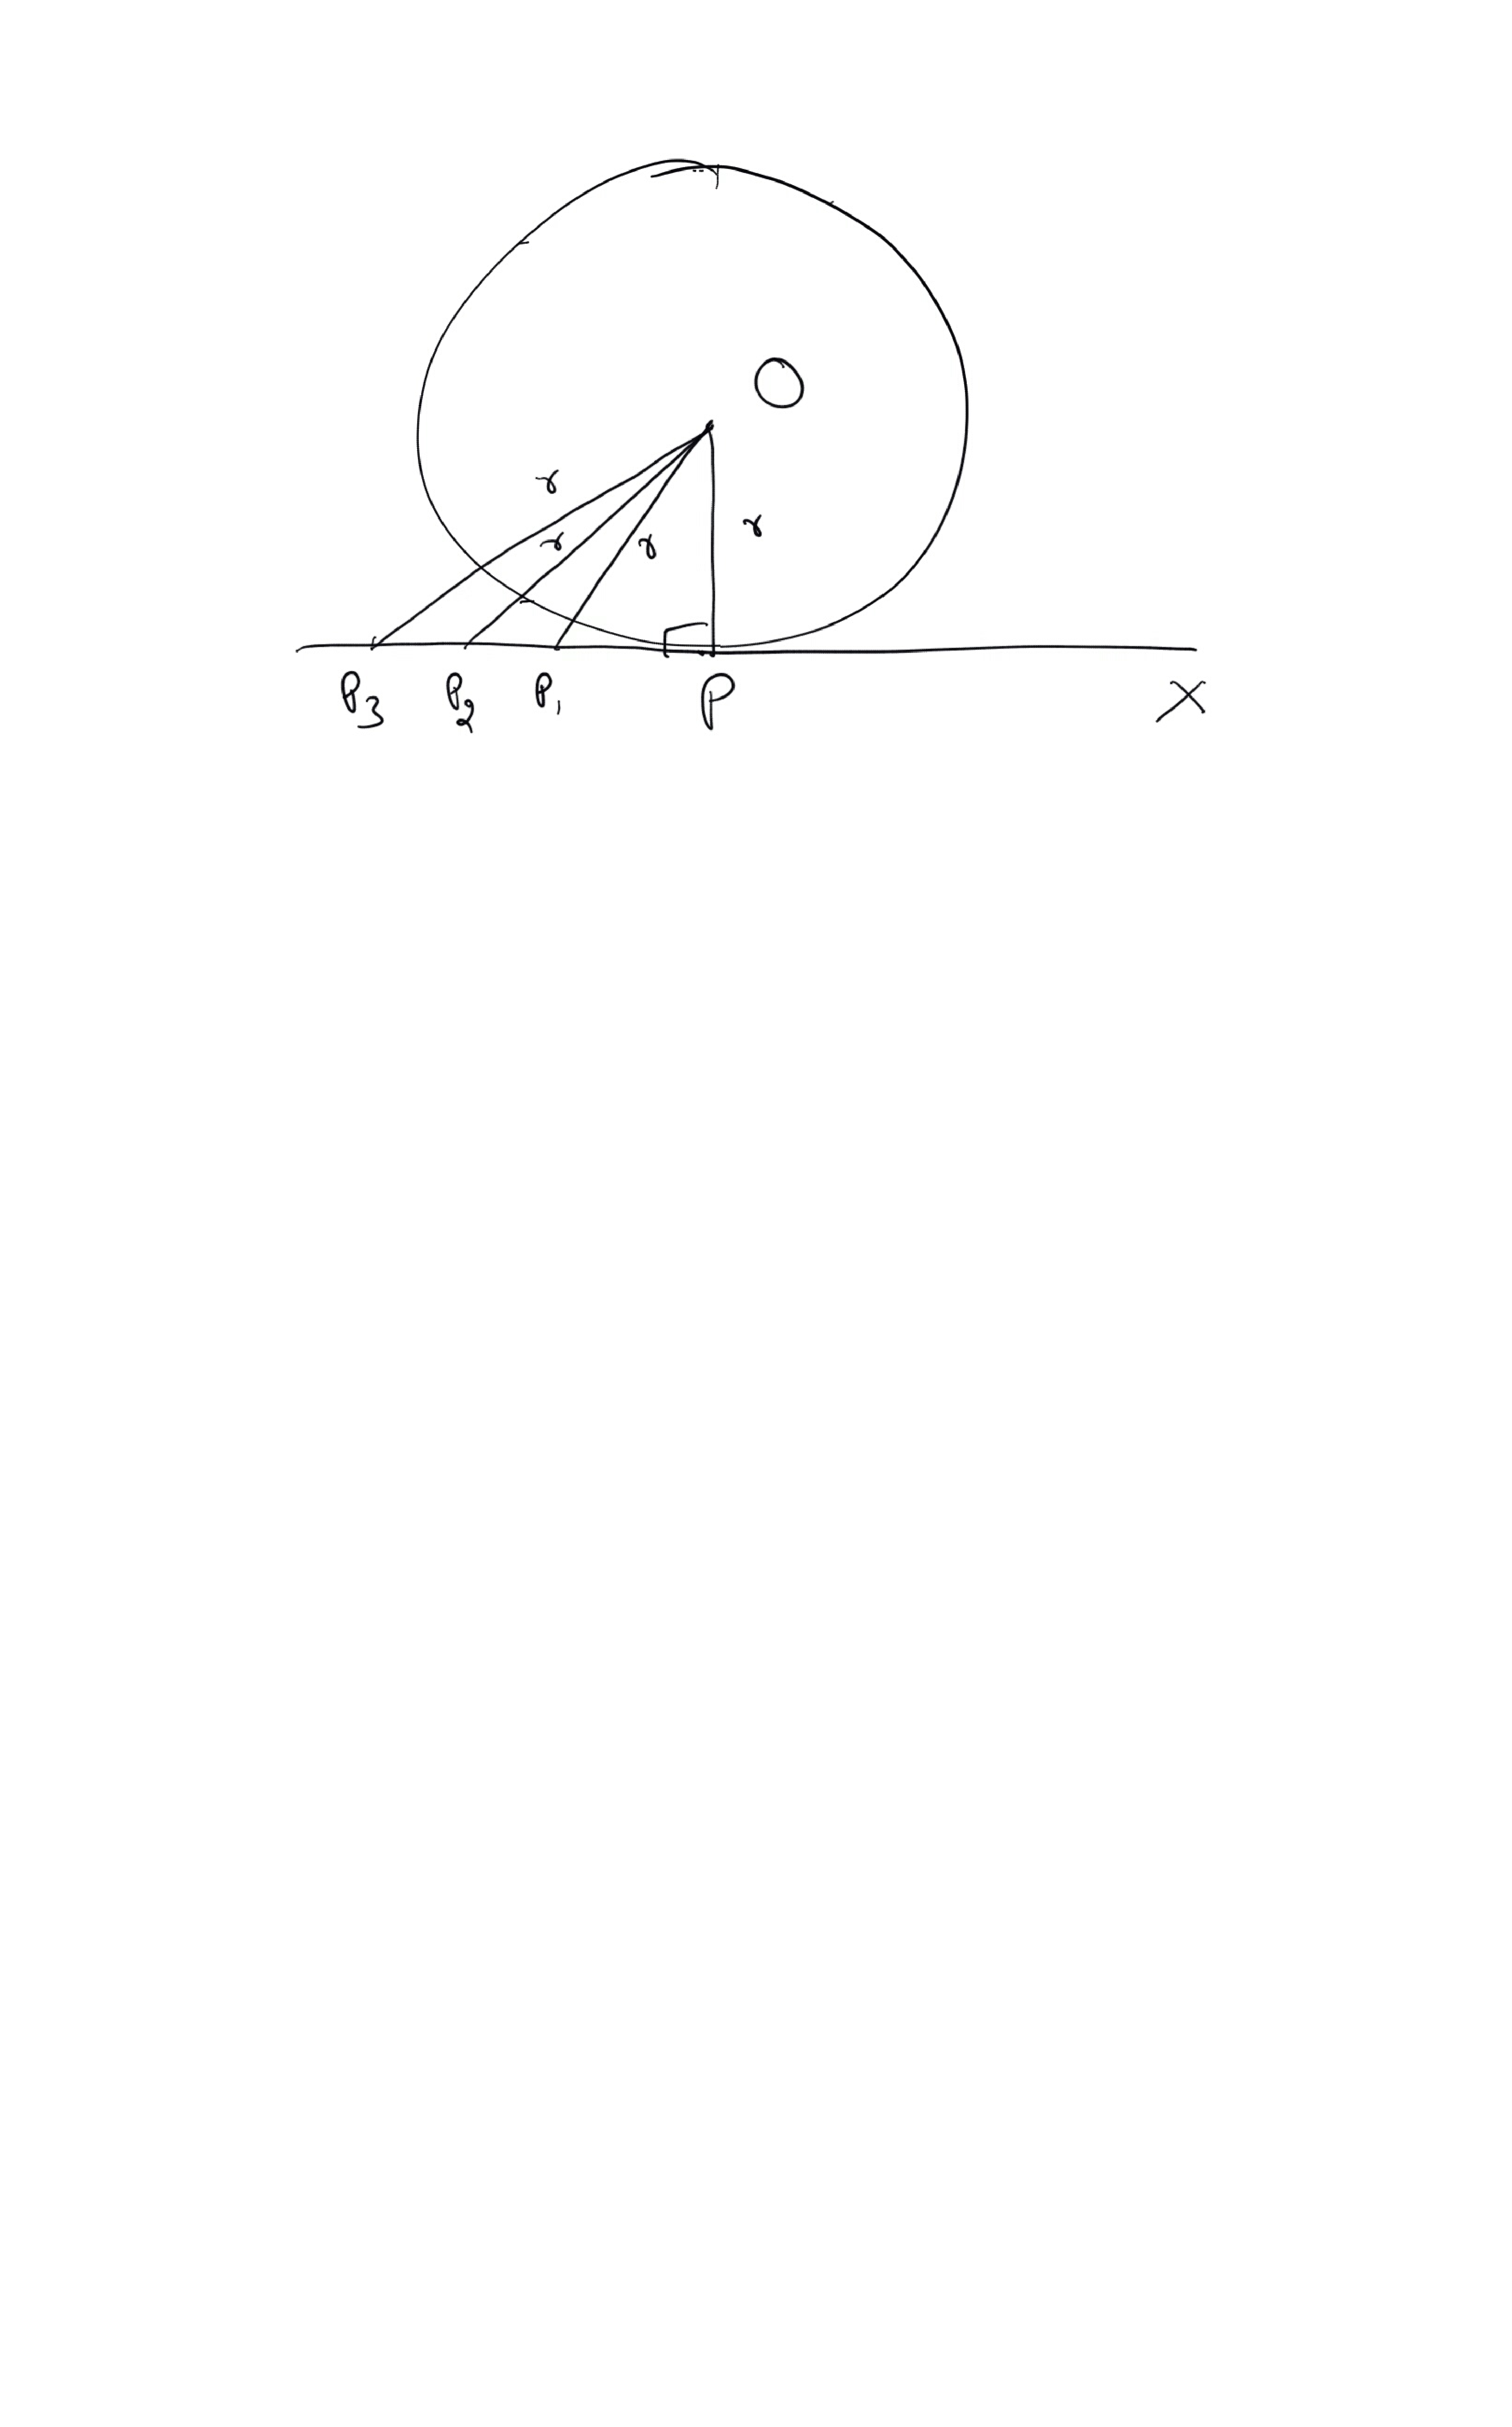
\includegraphics[width=\columnwidth]{./figs/ch4_tangent_def}
		%\vspace*{-10cm}
		\resizebox{\columnwidth}{!}{\begin{tikzpicture}
[scale =2,>=stealth,point/.style = {draw, circle, fill = black, inner sep = 1pt},]

\def\rad{2}
\coordinate [point, label={right: $O$ }] (O) at (0, 2);
\draw (O) circle (\rad);
\node (P) at (0,0)[point,label=below :$P$] {};
\node (X) at (2,0)[point,label=right :$X$] {};
\node (Y) at (-4,0)[point,label=left :$Y$] {};
\node (P_1) at (-1,0)[point,label=below  :$P_1$] {};
\node (P_2) at (-2,0)[point,label=below  :$P_2$] {};
\node (P_3) at (-3,0)[point,label=below  :$P_3$] {};

\draw (O)--(P);
\draw (X)--(Y);
\draw (O)--(P_1);
\draw (O)--(P_2);
\draw (O)--(P_3);

\tkzMarkRightAngle[size=.2](O,P,P_1);
\node [above] at (-0.8,0.5){$r$};
\node [above] at (-1.2,0.8){$r$};
\node [above] at (-1.45,1){$r$};
\node [above] at (0.1,0.8){$r$};
\end{tikzpicture}}
	\end{center}
	\caption{Tangent to a Circle.}
	\label{ch4_tangent_def}	
\end{figure}
%
%\begin{figure}[!ht]
%	\begin{center}
%		
%		%
\includegraphics[width=\columnwidth]{./figs/ch4_short_dist}
%		%\vspace*{-10cm}
%		\resizebox{\columnwidth}{!}{\begin{tikzpicture}
[scale =2,>=stealth,point/.style = {draw, circle, fill = black, inner sep = 1pt},]


\node (O) at (0,3)[point,label=above :$O$] {};
\node (P) at (0,0)[point,label=below :$P$] {};
\node (P_1) at (-1.5,0)[point,label=below :$P_1$] {};
\node (P_2) at (-3,0)[point,label=below :$P_2$] {};
\node (X) at (2,0)[point,label=right :$X$] {};
\node (Y) at (-4,0)[point,label=left :$Y$] {};
\draw (O)--(P);
\draw (X)--(Y);
\draw (O)--(P_1);
\draw (O)--(P_2);

\tkzMarkRightAngle[size=.2](O,P,X);

\end{tikzpicture}}
%	\end{center}
%	\caption{Shortest distance from $O$ to line $PX$}
%	\label{ch4_short_dist}	
%\end{figure}

%
\begin{align}
%\begin{split}
\brak{r+d_n}^2 = r^2 + x_n^2 - 2rx_n\cos\theta > r^2 
\\
\implies  0 <\cos\theta < \frac{x_n}{2r},
%OP_1^2 &= OP^2 + PP_1^2 \\
%\Rightarrow OP_1 > OP
%\end{split}
\end{align}
%
where $x_n$ can be made as small as we choose.  Thus, 
%
\begin{align}
\cos \theta = 0 \implies \theta  = 90 ^{\degree}
\end{align}
from \eqref{ch5_cos_90}.

%\solution In Fig. \ref{ch4_tangent_def}, we can see that $OP$ is is the radius of the circle and the length of all line segments from $O$ to the line $PX > r$.  Using the result of the previous 
%problem, it is obvious that $OP \perp PX$. 
%
	%
\item
In Fig. \ref{ch4_tangent_prod} show that 
%
\begin{equation}
\angle PCA = \angle PBC
\end{equation}
%
$O$ is the centre of the circle and $PC$ is the tangent.

	\begin{figure}[!ht]
		\begin{center}
			
			%
\includegraphics[width=\columnwidth]{./figs/ch4_tangent_prod}
			%\vspace*{-10cm}
			\resizebox{\columnwidth}{!}{\begin{tikzpicture}
[scale =2,>=stealth,point/.style = {draw, circle, fill = black, inner sep = 1pt},]

\def\rad{2}
\coordinate [point, label={above: $O$ }] (O) at (0, 2);
\draw (O) circle (\rad);
\node (P) at (-4,0)[point,label=below :$P$] {};
\node (C) at (0,0)[point,label=below :$C$] {};
\node (A) at (-1.92,1.45)[point,label=above left :$A$] {};
\node (B) at (1.2,3.6)[point,label=above right :$B$] {};
\draw (O)--(C);
\draw (P)--(C);
\draw (P)--(B);
\draw (A)--(C);
\draw (B)--(C);

\draw [thick,dashed](A)--(O);
\tkzMarkRightAngle[size=.2](P,C,O);
\tkzMarkAngle[size=.3](A,B,C);
\tkzMarkAngle[size=.4](O,C,A);
%\tkzMarkAngle[size=.5](B,C,O);
%\tkzMarkAngle[size=.3](P,A,C);
\tkzMarkAngle[size=.2](C,A,O);
\tkzMarkAngle[size=.2](A,O,C);

\node [above] at (0.65,1.5){$r$};
\node [above] at (-0.9,1.7){$r$};
\node [above] at (0.1,1){$r$};
%\draw (-1.9,1) node{$\theta$};

\draw (0.95,3.3) node{$\alpha$};
\draw (-0.2,1.7) node{$2\alpha$};
\draw (-0.2,0.5) node{$90-\alpha$};
\draw (-1.4,1.4) node{$90-\alpha$};
%\draw (.1,.6) node{$\phi$};

\end{tikzpicture}}
		\end{center}
		\caption{$PA.PB = PC^2$.}
		\label{ch4_tangent_prod}	
	\end{figure}
	%

%
\solution Obvious from the figure once we observe that $\triangle OAC$ is isosceles.
%
%
\item
	In Fig. \ref{ch4_tangent_prod}, show that the triangles $PAC$ and $PBC$ are similar.

\solution From the previous problem, it is obvious that corresponding angles of both triangles are equal.  Hence they are similar.
%
\item
	Show that $PA.PB = PC^2$

\solution Since $\Delta PAC \sim \Delta PBC$, their sides are in the same ratio.  Hence,
%
\begin{align}
\frac{PA}{PC} &= \frac{PC}{PB} \\
\Rightarrow PA.PB &=PC^2
\end{align}
%
\item
Given that $PA.PB = PC^2$, show that $PC$ is a tangent to the circle.

%
\item
	In Fig. \ref{ch4_chord_tangent_prod}, show that\begin{equation}
	PA.PB = PC.PD
	\end{equation}

%
\begin{figure}[!ht]
	\begin{center}
		
		%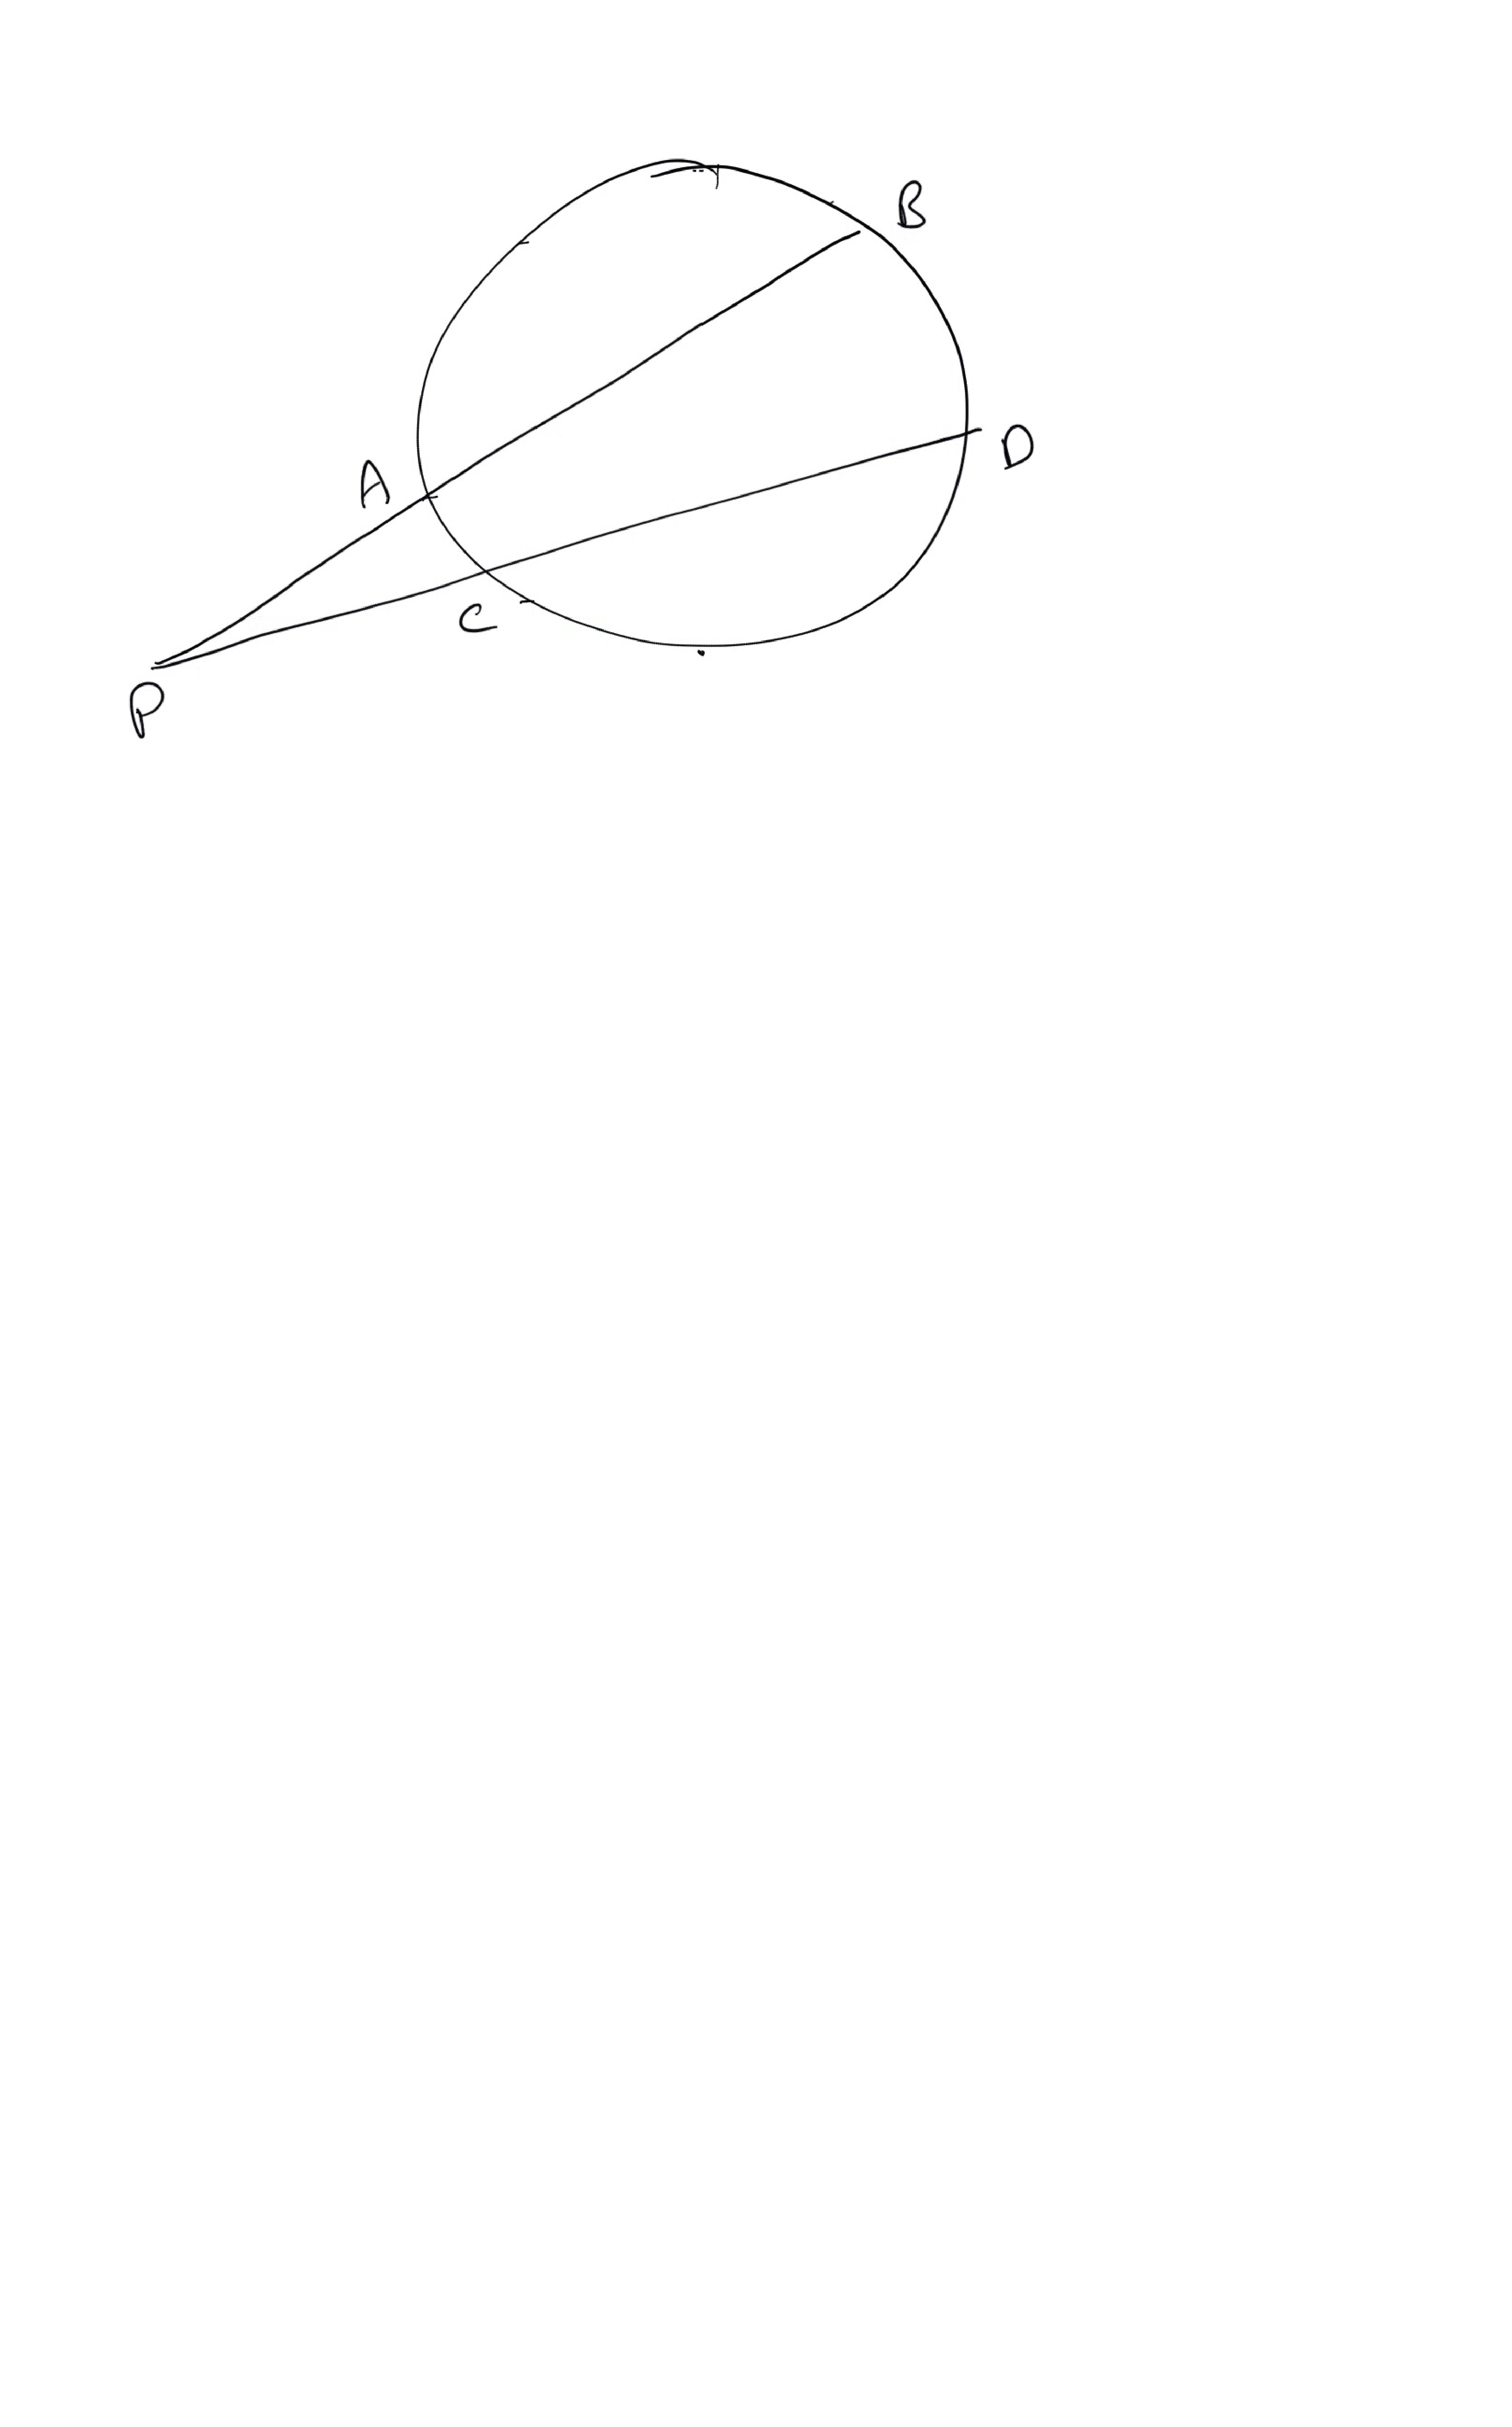
\includegraphics[width=\columnwidth]{./figs/ch4_chord_tangent_prod}
		%\vspace*{-10cm}
		\resizebox{\columnwidth}{!}{\begin{tikzpicture}
[scale =2,>=stealth,point/.style = {draw, circle, fill = black, inner sep = 1pt},]

\def\rad{2}
\coordinate [point, label={above: $O$ }] (O) at (0, 2);
\draw (O) circle (\rad);
\node (P) at (-5,0)[point,label=below :$P$] {};
\node (C) at (-1.65,0.9)[point,label=below :$C$] {};
\node (A) at (-2,2.3)[point,label=left :$A$] {};
\node (B) at (0.3,4)[point,label=above :$B$] {};
\node (D) at (2,2)[point,label=right :$D$] {};
\draw (C)--(D);
\draw (A)--(B);
\draw (A)--(P);
\draw (P)--(C);
\end{tikzpicture}}
	\end{center}
	\caption{$PA.PB = PC^2$.}
	\label{ch4_chord_tangent_prod}	
\end{figure}

\solution Draw a tangent and use the previous problem.
\end{enumerate}


%\subsection{Area of a Circle}
\subsection{Area of a Circle}
%
%
\renewcommand{\theequation}{\theenumi}
\begin{enumerate}[label=\arabic*.,ref=\thesubsection.\theenumi]
\numberwithin{equation}{enumi}
%
%
%\item
%	Using Fig. \ref{ch5_sin_theta}, show that 
%	%
%\begin{equation}
%\label{ch5_sin_theta_eq}
%\sin  \theta_1 = \sin \brak{\theta_1 + \theta_2}\cos \theta_2 - \cos\brak{\theta_1+\theta_2}\sin\theta_2
%\end{equation}	
%	%
%
%\begin{figure}[!ht]
%	\begin{center}
%		
%		%
\includegraphics[width=\columnwidth]{./figs/ch5_sin_theta}
%		%\vspace*{-10cm}
%		\resizebox{\columnwidth}{!}{\begin{tikzpicture}
[scale =3,>=stealth,point/.style = {draw, circle, fill = black, inner sep = 1pt},]

\node (A) at (0,3)[point,label=above :$A$] {};
\node (B) at (3,0)[point,label=below :$B$] {};
\node (C) at (0,0)[point,label=below :$C$] {};
\node (D) at (0,1.5)[point,label=left :$D$] {};
\draw (A)--(B);
\draw (C)--(B);
\draw (A)--(C);
\draw (B)--(D);
\tkzMarkAngle[size=.4](A,B,D);
\tkzMarkAngle[size=.3](D,B,C);
\tkzMarkRightAngle[size=.15](A,C,B);

\node [above] at (1.6,1.5){$c$};
\node [below] at (1.6,0){$a$};
\node [above] at (-0.2,1.5){$b$};
\node [above] at (2.5,0){$\theta_2$};
\node [above] at (2.5,0.3){$\theta_1$};
\end{tikzpicture}}
%	\end{center}
%	\caption{$\sin2\theta = 2\sin\theta\cos\theta$}
%	\label{ch5_sin_theta}	
%\end{figure}
%%
%
%\solution The following equations can be obtained from the figure using the forumula for the area of a triangle
%%
%\begin{align}
%ar \brak{\Delta ABC} &= \frac{1}{2}ac \sin\brak{\theta_1 + \theta_2} \\
%&= ar \brak{\Delta BDC} + ar \brak{\Delta ADB} \\
%&= \frac{1}{2}cl \sin{\theta_1} + \frac{1}{2}al \sin{\theta_2} \\ 
%&= \frac{1}{2}ac \sin{\theta_1} \sec \theta_2 + \frac{1}{2}a^2 \tan{\theta_2} 
%\end{align}
%$\brak{\because
%	l = a \sec \theta_2}$.  From the above,
%\begin{align}
%\Rightarrow \sin\brak{\theta_1 + \theta_2} &=  \sin{\theta_1} \sec \theta_2 + \frac{a}{c} \tan{\theta_2} \\
%\Rightarrow \sin\brak{\theta_1 + \theta_2} &=  \sin{\theta_1} \sec \theta_2 + \cos\brak{\theta_1 + \theta_2} \tan{\theta_2} 
%\end{align}
%Multiplying both sides by $\cos \theta_2$,
%\begin{align}
%\Rightarrow \sin\brak{\theta_1 + \theta_2}\cos{\theta_2} &=  \sin{\theta_1}  + \cos\brak{\theta_1 + \theta_2} \sin\theta_2  
%\end{align}
%%
%resulting in
%\begin{equation}
%\Rightarrow \sin \theta_1 = \sin\brak{\theta_1 + \theta_2}\cos{\theta_2} - \cos\brak{\theta_1 + \theta_2} \sin\theta_2 
%\end{equation}
%\item
%	Prove the following identities 
%	%
%	\begin{enumerate}
%\item 
%\begin{equation}
%		\label{ch5_sin_diff}
%\sin\brak{\alpha - \beta} = \sin \alpha \cos \beta - \cos \alpha \sin \beta.
%\end{equation}
%\item 
%\begin{equation}
%\cos\brak{\alpha + \beta} = \cos \alpha \cos \beta - \sin \alpha \sin \beta.
%		\label{ch5_cos_diff}
%\end{equation}
%
%	\end{enumerate}
%	%
%
%\solution In \eqref{ch5_sin_theta_eq}, let
%%
%\begin{equation}
%\begin{split}
%\theta_1 + \theta_2 &= \alpha \\
%\theta_2 &=  \beta
%\end{split}
%\end{equation}
%%
%This gives \eqref{ch5_sin_diff}.  In \eqref{ch5_sin_diff}, replace $\alpha$ by 
%%
%$90{\degree} - \alpha$.  This results in
%%
%\begin{multline}
%\sin\brak{90{\degree} - \alpha - \beta}
%\\
%=
%\sin \brak{90{\degree} -\alpha} \cos \beta - \cos \brak{90{\degree} -\alpha} \sin \beta \\
%\Rightarrow \cos\brak{\alpha + \beta} = \cos \alpha \cos \beta - \sin \alpha \sin \beta
%\end{multline}
%% 
%\item
%	Using \eqref{ch5_sin_theta_eq} and \eqref{ch5_cos_diff}, show that
%\begin{align}
%\label{ch5_sin_sum}
%\sin\brak{\theta_1 + \theta_2} &= \sin\theta_1  \cos\theta_2 + \cos\theta_1\sin\theta_2
%\\
%\cos\brak{\theta_1 - \theta_2} &= \cos\theta_1  \cos\theta_2  \sin\theta_1\sin\theta_2
%\label{ch5_cos_sum}
%\end{align}
%
%%
%\solution From \eqref{ch5_sin_theta_eq},
%%
%\begin{align}
% \sin \brak{\theta_1 + \theta_2}\cos \theta_2 =\sin  \theta_1 +\cos\brak{\theta_1+\theta_2}\sin\theta_2 
%\end{align}
%%
%Using \eqref{ch5_cos_diff} in the above,
%%
%\begin{multline}
%\sin \brak{\theta_1 + \theta_2}\cos \theta_2 
%=\sin  \theta_1 +\lbrak{\cos \theta_1\cos\theta_2 }
%\\	
%\rbrak{	- \sin \theta_1\sin\theta_2}\sin\theta_2 
%\end{multline}
%%
%which can be expressed as
%%
%\begin{multline}
%\sin \brak{\theta_1 + \theta_2}\cos \theta_2 
%=\sin  \theta_1 +\cos \theta_1\cos\theta_2 \sin\theta_2 
%\\	
%	- \sin \theta_1\sin^2\theta_2
%\end{multline}
%%
%Since
%%
%\begin{equation}
%\sin^2\theta_2 = 1- \cos^2\theta_2, 
%\end{equation}
%%
%we obtain
%%
%\begin{multline}
%\sin \brak{\theta_1 + \theta_2}\cos \theta_2 
%=\cos \theta_1\cos\theta_2 \sin\theta_2 
%\\	
%+ \sin \theta_1\cos^2\theta_2
%\end{multline}
%%
%resulting in
%%
%\begin{equation}
%\sin \brak{\theta_1 + \theta_2}
%=\cos \theta_1 \sin\theta_2 
%+ \sin \theta_1\cos\theta_2
%\end{equation}
%%
%after factoring out $\cos \theta_2$.  Using a similar approach, \eqref{ch5_cos_sum} can also be proved.
%%
%\item
%	Show that
%	%
%	\begin{equation}
%	\label{eq:sin2theta}
%	\sin 2\theta = 2 \sin\theta \cos\theta
%	\end{equation}
%	%
%%
%\item
%	Show that
%	%
%	\begin{align}
%	\label{eq:cos2theta_cos_sin}
%	\cos 2\theta &= \cos^2\theta -\sin^2\theta 
%\\
%	\label{eq:cos2theta_sin_sq}
%&= 1 - \sin^2\theta
%\\
%&=2\cos^2\theta -1
%	\label{eq:cos2theta_cos_sq}
%	\end{align}
%	%
\item The ratio of the perimeter of a circle to its diameter is $\pi$.
\label{prob:circ_peri_dia}
\item {\em Radian} is a another unit of the angle defined by
%
\begin{align}
\pi \text{ radians} = 180 \degree
\end{align}
%
\item
	In Fig. \ref{ch5_polygon_def}, 6 congruent triangles are arranged in a circular fashion.  Such a figure is known as a regular hexagon.  In general, $n$ number of traingles can be arranged to form a regular polygon.
\begin{figure}[!ht]
	\begin{center}
		
		%
\includegraphics[width=\columnwidth]{./figs/ch5_polygon_def}
		%\vspace*{-10cm}
		\resizebox{\columnwidth}{!}{\begin{tikzpicture}
[scale =2,>=stealth,point/.style = {draw, circle, fill = black, inner sep = 1pt},]

\node (O) at (0,0)[point,label=above :$O$] {};
\node (F) at (-3,0)[point,label=left :$F$] {};
\node (C) at (3,0)[point,label=right :$C$] {};
\node (E) at (-1.5,3)[point,label=above :$E$] {};
\node (D) at (1.5,3)[point,label=above :$D$] {};
\node (A) at (-1.5,-3)[point,label=below :$A$] {};
\node (B) at (1.5,-3)[point,label=below :$B$] {};
\draw (A)--(D);
\draw (B)--(E);
\draw (F)--(C);
\draw (A)--(F);
\draw (F)--(E);
\draw (E)--(D);
\draw (D)--(C);
\draw (C)--(B);
\draw (B)--(A);

\tkzMarkAngle[size=.2](F,O,A);
\tkzMarkAngle[size=.22](E,O,F);
\tkzMarkAngle[size=.26](D,O,E);
\tkzMarkAngle[size=.2](C,O,D);
\tkzMarkAngle[size=.22](B,O,C);
\tkzMarkAngle[size=.26](A,O,B);

\node [above] at (-0.8,-1.5){$r$};
\node [above] at (-1.5,0){$r$};
\node [above] at (-0.9,1.5){$r$};
\node [above] at (0.9,1.5){$r$};
\node [above] at (1.5,0){$r$};
\node [above] at (0.8,-1.5){$r$};
\node [above] at (0,-0.7){$\frac{2\pi}{6}$};

\end{tikzpicture}
}
	\end{center}
	\caption{Polygon Definition}
	\label{ch5_polygon_def}	
\end{figure}
%
\item
The angle formed by each of the congruent triangles at the centre of a regular polygon of $n$ sides is $\frac{2\pi}{n} = \frac{2\pi}{n}$ rad.
%
\item 	The triangle that forms a polygon of $n$ sides is given in Fig. \ref{ch5_polygon_area}. Show that 
%
\begin{equation}
BC = 2r \sin\frac{\pi}{n}
\label{eq:circ_chord_len}
\end{equation}
%

\begin{figure}[!ht]
	\begin{center}
		
		%
\includegraphics[width=\columnwidth]{./figs/ch5_polygon_area}
		%\vspace*{-10cm}
		\resizebox{\columnwidth}{!}{\begin{tikzpicture}
[scale =2,>=stealth,point/.style = {draw, circle, fill = black, inner sep = 1pt},]

\node (A) at (0,3)[point,label=above :$A$] {};
\node (B) at (-3,0)[point,label=below :$B$] {};
\node (C) at (3,0)[point,label=below :$C$] {};
\draw (A)--(B);
\draw (C)--(B);
\draw (A)--(C);

\tkzMarkAngle[size=.2](B,A,C);
\node [above] at (0.05,2.5){$\frac{2\pi}{n}$};
\node [above] at (-1.6,1.5){$r$};
\node [above] at (1.6,1.5){$r$};
\end{tikzpicture}
}
	\end{center}
	\caption{Triangle that forms a polygon}
	\label{ch5_polygon_area}	
\end{figure}
%
%\\
\solution Using cosine formula, 
%
%
\begin{align}
BC^2 &= 2r^2-2r^2 \cos\frac{2\pi}{n}
\\
\implies BC^2 &= 2r^2\brak{1-\cos\frac{2\pi}{n}}
&= 4r^2\sin^2\frac{\pi}{n}
\end{align}
%
upon substituting from 	\eqref{eq:cos2x}
%\eqref{eq:cos2theta_sin_sq}.  
Taking the square root results in \eqref{eq:circ_chord_len}
%
\item
Show that the perimeter of a regular polygon is given by 
%
\begin{equation}
\label{eq:peri_poly_n}
2rn \sin\frac{\pi}{n}
\end{equation}
%
\item
Show that the area of a regular polygon is given by 
%
\begin{equation}
\frac{n}{2}r^{2}\sin\frac{2\pi}{n}
\end{equation}
%
\solution  From Fig. 	\ref{ch5_polygon_area}	

%
\begin{equation}
\begin{split}
ar\brak{polygon} &= n \times ar\brak{\Delta ABC} \\
&= \frac{n}{2}r^{2}\sin\frac{2\pi}{n}
\end{split}
\end{equation}
%
\item
	Using Fig. \ref{ch5_circle_squeeze}, show that
%
\begin{equation}
\label{ch5_circle_squeeze_eq}
\frac{n}{2}r^{2}\sin\frac{2\pi}{n} < \text{ area of circle } < nr^{2}\tan\frac{\pi}{n}
\end{equation}
%
The portion of the circle visible in Fig. \ref{ch5_circle_squeeze} is defined to be a sector of the circle.

\begin{figure}[!ht]
	\begin{center}
		
		%
\includegraphics[width=\columnwidth]{./figs/ch5_circle_squeeze}
		%\vspace*{-10cm}
		\resizebox{\columnwidth}{!}{\begin{tikzpicture}
[scale =2,>=stealth,point/.style = {draw, circle, fill = black, inner sep = 1pt},]

\def\rad{3}
\coordinate [point, label={right: $O$ }] (O) at (0, 0);
\draw (O) circle (\rad);
\node (P) at (0,-3)[point,label=below :$P$] {};
\node (A) at (-2,-2.22)[point,label= left :$A$] {};
\node (B) at (2,-2.22)[point,label=right :$B$] {};
\node (C) at (-2.7,-3)[point,label=below :$C$] {};
\node (D) at (2.7,-3)[point,label=below :$D$] {};
\draw (A)--(B);
\draw (O)--(B);
\draw (A)--(O);
\draw (O)--(P);
\draw (C)--(P);
\draw (D)--(P);

\draw [thick,dashed](A)--(C);
\draw [thick,dashed](B)--(D);
\tkzMarkRightAngle[size=0.2](O,P,D)
\tkzMarkAngle[size=0.2](C,O,P)
\tkzMarkAngle[size=0.3](P,O,D)
\node [above] at (-1.4,-1.5){$r$};
\node [above right] at (0,-1.5){$r$};
\node [above] at (1.4,-1.5){$r$};
\node [above right] at (0.4,-0.5){$\theta=360/n$};
\end{tikzpicture}}
	\end{center}
	\caption{Circle Area in between Area of Two Polygons}
	\label{ch5_circle_squeeze}	
\end{figure}
%

\solution Note that the circle is squeezed between the inner and outer regular polygons.  As we can see from Fig. \ref{ch5_circle_squeeze}, the area of the circle should be in between the areas of the inner and outer polygons.  Since
%
\begin{align}
ar \brak{\Delta OAB} &= \frac{1}{2}r^{2}\sin\frac{2\pi}{n} \\
ar \brak{\Delta OPQ} &= 2 \times \frac{1}{2} \times r \tan\frac{2\pi/n}{2} \times r \\
&= r^{2}\tan\frac{\pi}{n},
\end{align}
%
we obtain \eqref{ch5_circle_squeeze_eq}.
%
\item
Show that
	%
	\begin{equation}
	\label{ch5_circle_squeeze_simple}
\cos^2\frac{\pi}{n} < \frac{\text{ area of circle }}{nr^{2}\tan\frac{\pi}{n}} < 1	\end{equation}
	%

\solution From \eqref{ch5_circle_squeeze_eq} and \eqref{eq:sin2theta},
	%
{\small
	\begin{align}
	\frac{n}{2}r^{2}\sin\frac{2\pi}{n} < \text{ area of circle } 
%	\\
	< nr^{2}\tan\frac{\pi}{n} 
	\\
\Rightarrow 	
	{n}r^{2}\sin\frac{\pi}{n}\cos\frac{\pi}{n} < \text{ area of circle } 
%	\\
	< nr^{2}\tan\frac{\pi}{n} 
	\end{align}
%
}
which yields 	\eqref{ch5_circle_squeeze_simple} upon making use of the fact that 
%
\begin{align}
\frac{\sin \theta}{\cos \theta} = \tan \theta
\end{align}
%

%
\item
	Show that 
	\begin{equation}
	\label{ch5_cos_zero}
	\cos 0^{\degree} = 1
	\end{equation}

\solution Follows from the fact that $\cos 0 \degree = \sin \brak{90\degree -0\degree} = \sin \brak{90\degree }=1$ using \eqref{eq:tri_90-ang}.


%From \eqref{ch1_trig_defs}, $\theta \to 0\degree \implies a \to 0 \implies \sin \theta $ and %

\item
	Show that 
	\begin{equation}
	\label{ch5_sin_zero}
	\sin 0^{\degree} = 0
	\end{equation}
%\solution Follows from the fact that $\sin 0 = 0$ and \eqref{eq:tri_sin_cos_id}.

\item
	Show that for large values of $n$
	%
	\begin{equation}
\label{eq:cos_zero_lim}
	%
\cos^2\frac{\pi}{n} = 1
%
	\end{equation}	
	% 

%
\solution  As $n \to \infty, \frac{\pi}{n} \to 0$. From \eqref{ch5_cos_zero}, this yields \eqref{eq:cos_zero_lim}.

%
\item  \eqref{eq:cos_zero_lim} is a {\em limit} and 
	 expressed as 
%
\begin{equation}
\label{eq:cos_zero_lim_def}
\lim_{n \rightarrow \infty}\cos^2\frac{\pi}{n} = 1
\end{equation}
%	

\item
	Show that 
	%
\begin{equation}
\label{ch5_circle_squeeze_tan_n}
\text{ area of circle } = r^2\lim_{n \rightarrow \infty}
{n\tan\frac{\pi}{n}} 
	%
\end{equation}	
	% 
\solution From \eqref{ch5_circle_squeeze_simple} and \eqref{eq:cos_zero_lim_def}, 
	%
	\begin{align}
%	\label{ch5_circle_squeeze_simple}
\lim_{n\to \infty}\cos^2\frac{\pi}{n} < \lim_{n\to \infty} \frac{\text{ area of circle }}{nr^{2}\tan\frac{\pi}{n}} < 1	
\\
1 = \lim_{n\to \infty} \frac{\text{ area of circle }}{nr^{2}\tan\frac{\pi}{n}} < 1	
\end{align}
	%
resulting in \eqref{ch5_circle_squeeze_tan_n}.
%

%
\item Show that 

	\begin{equation}
\label{eq:peri_poly_tan_n}
	\pi = \lim_{n \rightarrow \infty}
	{n\tan\frac{\pi}{n}}
	\end{equation}
\solution From \eqref{prob:circ_peri_dia} and \eqref{eq:peri_poly_n}, the perimeter of the circle is 
%
\begin{align}
\label{eq:peri_poly_sin_n}
\lim_{n\to \infty}2rn \sin\frac{\pi}{n} &= 2\pi r
\implies \lim_{n\to \infty}n \sin\frac{\pi}{n} &= \pi 
\end{align}
%
Also, from Fig. \eqref{ch5_circle_squeeze}, using the fact that the inner and outer polygons converge into a circle for large $n$,
\begin{align}
%\label{eq:peri_poly_n}
\lim_{n\to \infty} nCD -nAB &= 0
\\
\implies \lim_{n\to \infty} 2r n\tan\frac{\pi}{n}-2r n\sin\frac{\pi}{n} &= 0
\end{align}
%
from which, we obtain \eqref{eq:peri_poly_tan_n}
by substituting from \eqref{eq:peri_poly_sin_n}.


\item Show that the area of a circle is $\pi r^2$.
\\
\solution Use \eqref{eq:peri_poly_tan_n} in \eqref{ch5_circle_squeeze_tan_n}.

%\item
%	The radian is a unit of angle defined by
%\begin{equation}
%	1 \text{ radian} = \frac{2\pi}{2\pi}
%\end{equation}

%
%\item
%	Show that the circumference of a circle is $2 \pi r$.
\item
	Show that
	\begin{equation}
	\lim_{\theta \rightarrow 0} \frac{\sin\theta}{\theta} =
	\lim_{\theta \rightarrow 0} \frac{\tan\theta}{\theta} = 1
	\end{equation}

\item
	Show that the area of a sector with angle $\theta$ in radians is $\frac{1}{2}r^2\theta$.


\end{enumerate}

%

%
\section{Exercises}
%

\subsection{Triangle Exercises}
\renewcommand{\theequation}{\theenumi}
\begin{enumerate}[label=\arabic*.,ref=\thesubsection.\theenumi]
\numberwithin{equation}{enumi}
%\chapter{The Optimum Receiver}
%\item Angles opposite to equal sides of a triangle are equal. 
%\label{prob:tri_ang_side_eq}
%\\
%\solution Using the sine formula in \eqref{eq:tri_sin_form},%
%\begin{align}
%\frac{\sin A}{a} = \frac{\sin B}{b}
%\end{align}
%%
%Thus, if $A=B$, $\sin A = \sin B \implies a =b$.
%\\
%\solution Use \eqref{eq:tri_sin_form} and the argument in Problem \ref{prob:tri_ang_side_eq}
%
\item  Each angle of an equilateral triangle is of 60$\degree$. 
%\\
%\solution In an equilateral $\triangle$, 
%%
%\begin{align}
%A=B=C.&
%\\
%\because A+B+C = 180\degree, 3A = 180\degree&
%\\
%\implies A = 60\degree&
%\end{align}
%


%\subsection{Problem}
\item Triangles on the same base (or equal bases) and between the same parallels are equal in area.
\item Triangles on the same base (or equal bases) and having equal areas lie between the same parallels.
\item In $\triangle ABC, D, E$ and $F$ are respectively the mid-points of sides $AB, BC$ and $CA $. Show that $\triangle ABC$ is divided into four congruent triangles by joining $D, E$ and $F$.
\item  The line-segment joining the mid-points of any two sides of a triangle is parallel to the third side and is half of it.
\label{prob:tri_mid_similar}
%\label{prob:quad_similar}
%%
%\\
%\solution If $DE$ is the lie joining he mid points of $\triangle ABC$,  use cosine formula to find the lengths of $DE$ and $BC$. Then use cosine formula to show that all angles of $\triangle ADE$ are equal to the corresponding angles of $\triangle ABC$.
%
\item  A line through the mid-point of a side of a triangle parallel to another side bisects the third side.
%\\
%\solution Use cosine formula.
\item ABC is a triangle right angled at $C$. A line through the mid-point $M$ of hypotenuse $AB$ and parallel to $BC$ intersects $AC$ at $D$. Show that (i) $D$ is the mid-point of $AC$
(ii) $MD \perp AC$ (iii) $CM = MA = \frac{1}{2}AB$

\item  Sides opposite to equal angles of a triangle are equal. 
%\\
%\solution Use \eqref{eq:tri_sin_form} and the argument in Problem \ref{prob:tri_ang_side_eq}
%
\item  Each angle of an equilateral triangle is of 60$\degree$. 
%\\
%\solution In an equilateral $\triangle$, 
%%
%\begin{align}
%A=B=C.&
%\\
%\because A+B+C = 180\degree, 3A = 180\degree&
%\\
%\implies A = 60\degree&
%\end{align}
%
\item Using cosine formula in an equilateral $\triangle$, show that $\cos 60\degree = \frac{1}{2} $.  
\item Using \eqref{eq:tri_sin_cos_id}, show that $\sin 60\degree = \frac{\sqrt{3}}{2} $.
\item Find  $\sin 30\degree$ and  $\sin 30\degree$ using \eqref{eq:tri_90-ang}.
%\subsection{Problem}
\item Triangles on the same base (or equal bases) and between the same parallels are equal in area.
\item Triangles on the same base (or equal bases) and having equal areas lie between the same parallels.
\item In $\triangle ABC$, the bisector $AD$ of $\angle  A$ is perpendicular to side $BC$. Show that $AB = AC$ and $\triangle ABC$ is isosceles.
\item $E$ and $F$ are respectively the mid-points of equal sides $AB$ and AC of $\triangle ABC$. Show that $BF = CE$. 
\item In an isosceles $\triangle ABC$ with $AB$ = AC, D and E are points on $BC$ such that $BE = CD$. Show that $AD = AE$. 
%
\item $AB$ is a line-segment. $P$ and $Q$ are points on opposite sides of $AB$ such that each of them is equidistant from the points $A$ and $B$. Show that the line $PQ $ is the perpendicular bisector of $AB$.
%
\item $P$ is a point equidistant from two lines $l$ and $m$ intersecting at point $A$.  Show that the line  $AP$  bisects the angle between them.
%
\item $D$ is a point on side $BC$ of $\triangle  ABC$ such that $AD = AC$. Show that $AB > AD$

%
\item $AB$ is a line segment and line $l$ is its perpendicular bisector. If a point $P$ lies on $l$, show that $P$ is equidistant from $A$ and $B$.
\item Line-segment $AB$ is parallel to another line-segment $CD$. $O$ is the mid-point of $AD$. Show that 
\begin{enumerate}
\item  $\triangle AOB \cong \triangle DOC$ 
\item  $O$ is also the mid-point of $BC$.
\end{enumerate}
%
\item In quadrilateral $ACBD, AC = AD$ and $AB$ bisects $\angle  A$. Show that $\triangle  ABC \cong \triangle  ABD$. What can you say about $BC$ and $BD$?
%
\item $ABCD$ is a quadrilateral in which $AD = BC$ and $\angle  DAB = \angle  CBA$ . Prove that
\begin{enumerate}
\item  $\triangle  ABD \cong  \triangle  BAC $
\item $ BD = AC $
\item  $\angle  ABD = \angle  BAC$.
\end{enumerate}
%
\item $l$ and $m$ are two parallel lines intersected by another pair of parallel lines p and q 
to form the quadrilateral $ABCD$. Show that $\triangle  ABC \cong  \triangle  CDA$.
%
\item Line $l$ is the bisector of $ \angle  A$ and $B$ is any point on $l$. $BP$ and $BQ$ are perpendiculars from $B$ to the arms of $\angle  A$ (see Fig. 7.20). Show that: 
\begin{enumerate}
\item  $\triangle  APB \cong  \triangle  AQB$ 
\item  $BP = BQ$ or $B$ is equidistant from the arms of $\angle  A$.
\end{enumerate}
%
\item $ABCE$ is a quadrilateral and $D$ is a point on $BC$ such that, $AC = AE, AB = AD$ and $\angle  BAD = \angle  EAC$. Show that $BC = DE$.
%
\item In right triangle $ABC$, right angled at $C, M$ is the mid-point of hypotenuse $AB$. $C$ is joined to $M$ and produced to a point $D$ such that $DM = CM$. Point $D$ is joined to point $B$.
Show that: 
\begin{enumerate}
\item $ \triangle  AMC \cong  \triangle  BMD $
\item $\angle  DBC$ is a right angle. 
\item $\triangle  DBC \cong  \triangle  ACB$
\item $ CM = \frac{1}{ 2} AB$
\end{enumerate}
%
\item In an isosceles $\triangle ABC$, with $AB = AC$, the bisectors of $\angle B$ and $\angle C$ intersect each other at $O$. Join $A$ to $O$. Show that :
\begin{enumerate} 
\item $OB = OC$ 
\item $AO$ bisects $\angle A$
\end{enumerate}
\item In $\triangle ABC$, $AD$ is the perpendicular bisector of $BC$. Show that $\triangle ABC$ is an isosceles triangle in which $AB = AC$.
\item $ABC$ is an isosceles triangle in which altitudes $BE$ and $CF$ are drawn to equal sides $AC$ and $AB$ respectively . Show that these altitudes are equal.
%
\item $ABC$ is a triangle in which altitudes $BE$ and $CF$ to sides $AC$ and $AB$ are equal. Show that
%
\begin{enumerate} 
\item $\triangle  ABE \cong  \triangle  ACF $
\item  $AB = AC$, i.e., $ABC$ is an isosceles triangle.
\end{enumerate}
%
\item $ABC$ and $DBC$ are two isosceles triangles on the same base $BC$. Show that $\angle ABD = \angle ACD$.
%
\item  $\triangle  ABC$ and $\triangle  DBC$ are two isosceles triangles on the same base $BC$ and vertices $A$ and $D$ are on the same side of $BC$. If $AD$ is extended to intersect $BC$ at $P$, show that
\begin{enumerate}
\item $\triangle  ABD \cong  \triangle  ACD $
\item $\triangle  ABP \cong  \triangle  ACP $
\item $AP$ bisects $\angle  A$ as well as $\angle  D$. 
\item $AP$ is the perpendicular bisector of $BC$.
\end{enumerate}
\item $AD$ is an altitude of an isosceles $\triangle ABC$ in which $AB = AC$. Show that 
\begin{enumerate}
\item $AD$ bisects $BC$
\item $AD$ bisects $\angle  A$. 
\end{enumerate}

\item  Two sides $AB$ and $BC$ and median $AM$ of one triangle $ABC$ are respectively equal to sides $PQ$ and $QR$ and median $PN$ of $\triangle  PQR$. Show that: 
\begin{enumerate}
\item $\triangle  ABM \cong  \triangle  PQN $
\item $\triangle  ABC \cong  \triangle  PQR$
\end{enumerate}
\item  $BE$ and $CF$ are two equal altitudes of a triangle $ABC$. Using RHS congruence rule, prove that the triangle $ABC$ is isosceles.
\item  $ABC$ is an isosceles triangle with $AB = AC$. Draw $AP \perp BC$ to show that $\angle  B = \angle  C$.
%
\item $\triangle ABC$ is an isosceles triangle in which $AB = AC$. Side $BA$ is produced to $D$ such that $AD = AB$. Show that $\angle BCD$ is a right angle.
%
\item $ABC$ is a right angled triangle in which $\angle A$ = 90$\degree$ and $AB = AC$. Find $\angle B$ and $\angle C$.
%
\item Show that in a right angled triangle, the hypotenuse is the longest side.
\item Sides AB and AC of $\triangle  ABC$ are extended to points P and Q respectively. Also, $\angle  PBC < \angle  QCB$. Show that $AC > AB$.

\item Line segments $AD$ and $BC$ intersect at $O$ and form $\triangle OAB$ and $\triangle ODC$. $\angle  B < \angle  A$ and $\angle  C < \angle  D$. Show that $AD < BC$.

\item $AB$ and $CD$ are respectively the smallest and longest sides of a quadrilateral $ABCD$. Show that $\angle  A > \angle  C$ and $\angle  B > \angle  D$.
%
\item In $\triangle PQR,  PR > PQ$ and $PS$ bisects $\angle  QPR$. Prove that $\angle  PSR > \angle  PSQ$.
%
\item Show that of all line segments drawn from a given point not on it, the perpendicular line segment is the shortest.
%
\item $ABCD$ is a trapezium with $AB  \parallel  DC$. $E$ and $F$ are points on non-parallel sides $AD$ and $BC$ respectively such that $EF$ is parallel to $AB$
. Show that
$\frac{AE}{ED}=\frac{ BF}{  FC}$ .
\item $ST$ is a line joining two points on $PQ$ and $PR$ in $\triangle PQR$.  If $\frac{PS}{ SQ}=\frac{PT}{ TR}$ and $ \angle  PST = \angle  PRQ$, prove that $PQR$ is an isosceles triangle.
%
\item If $LM  \parallel  CB$ and $LN  \parallel  CD$, prove that $\frac{AM}{AB} = \frac{ AN}{AD}$.
%
\item $D$ is a point on $AB$ and $E, F$ are points on $BC$ such that $DE  \parallel  AC$ and $DF  \parallel  AE$. Prove that $\frac{BF} {FE} =\frac{BE}  {EC}$.
%
\item $O$ is a point in the interior of $\triangle PQR$. $D$ is a point on $OP$.  If $DE  \parallel  OQ$ and $DF  \parallel  OR$. Show that $EF  \parallel  QR$.
\item $O$ is a point in the interior of $\triangle PQR$.  $A, B and C$ are points on $OP, OQ$ and $OR$ respectively such that $AB  \parallel  PQ$ and $AC  \parallel  PR$. Show that $BC  \parallel  QR$.
%
\item $ABCD$ is a trapezium in which $AB  \parallel  DC$ and its diagonals intersect each other at the point $O$. Show
that
$\frac{AO}{ BO}=\frac{CO}{  DO}$
%
\item The diagonals of a quadrilateral $ABCD$ intersect each other at the point $O$ such that $\frac{AO}{ BO}=\frac{CO}{  DO}$.   Show that $ABCD$ is a trapezium.
%
\item $PQ \parallel RS$ and $PS$ intersects $QR$ at $O$.  Show that $\triangle OPQ \sim \triangle ORS$.
 \item $CM$ and $RN$ are respectively the medians of $ \triangle  ABC$ and $ \triangle  PQR$. If $ \triangle  ABC  \sim   \triangle  PQR$, prove that 
\begin{enumerate}
\item  $ \triangle  AMC  \sim   \triangle  PNR$ 
\item  $\frac{CM}{RN}=\frac{ AB}{  PQ}$
\item $ \triangle  CMB  \sim   \triangle  RNQ$
%
\end{enumerate}
\item Diagonals $AC$ and $BD$ of a trapezium $ABCD$ with $AB  \parallel  DC$ intersect each other at the point $O$. Using a similarity criterion for two triangles, show that
$\frac{OA}{OC} =  \frac{OB}  {OD}$
%
\item In $\triangle PQR$, $QP$ is extended to $T$ and $S$ is a point on $QR$ such that $ \frac{QR}{QS}=\frac{ QT}{  PR}$. If $\angle PRQ = \angle PQS$, show that 
 that  $\triangle  PQS  \sim   \triangle  TQR$.
\item $S$ and $T$ are points on sides $PR$ and $QR$ of $\triangle PQR$ such that $\angle P = \angle 
 RTS$. Show that $\triangle RPQ \sim \triangle RTS$.
\item  In $\triangle ABC$, $D$ and $E$ are points on the sides $AB$ and $AC$ respectively.  If  $\triangle  ABE \cong   \triangle  ACD$, show that  $\triangle  ADE  \sim   \triangle  ABC$.
\item   Altitudes $AD$ and CE of  $\triangle  ABC$ intersect each other at the point $P$. Show that:
%
\begin{enumerate}
\item   $\triangle  AEP  \sim   \triangle  CDP $
\item   $\triangle  ABD  \sim   \triangle  CBE $
\item   $\triangle  AEP  \sim   \triangle  ADB$
 \item  $\triangle  PDC  \sim   \triangle  BEC$
\end{enumerate}
%
\item  $E$ is a point on the side $AD$ produced of a parallelogram $ABCD$ and $BE$ intersects $CD$ at $F$. Show that  $\triangle  ABE  \sim   \triangle  CFB$.
\item  $ABC$ and $AMP$ are two right triangles, right angled at $B$ and $M$ respectively. $M$ lies on $AC$ and $AB$ is extended to meet $P$. Prove that: 
\begin{enumerate}
\item   $\triangle  ABC  \sim   \triangle  AMP$
\item  $\frac{CA}{PA} = \frac{BC}{  MP}$
\end{enumerate}
%
\item  $CD$ and $GH$ are respectively the bisectors of  $\angle  ACB$ and  $\angle  EGF$ such that $D$ and $H$ lie on sides $AB$ and $FE$ of  $\triangle  ABC$ and  $\triangle  EFG$ respectively. If  $\triangle  ABC  \sim   \triangle  FEG$, show that:
\item  $\frac{CD}{GH} = \frac{ AC}{  FG}$
\item  $ \triangle  DCB  \sim   \triangle  HGE$
 \item  $ \triangle  DCA  \sim   \triangle  HGF$
\item  $E$ is a point on side $CB$ produced of an isosceles $\triangle ABC$ with $AB = AC$. If $AD  \perp  BC$ and $EF  \perp  AC$, prove that  $\triangle  ABD  \sim   \triangle  ECF$.
\item  Sides $AB$ and $BC$ and median $AD$ of a $\triangle ABC$ are respectively proportional to sides  $PQ$  and $QR$ and median $PM$ of  $\triangle PQR$. Show that  $\triangle  ABC  \sim  \triangle PQR$ .
\item  $D$ is a point on the side $BC$ of a $\triangle ABC$ such that  $\angle  ADC =  \angle  BAC$. Show that $CA^2 = CB.CD$.
\item  Sides $AB$ and $AC$ and median $AD$ of a $\triangle ABC$ are respectively proportional to sides $PQ$ and $PR$ and median $PM$ of another $\triangle PQR$. Show that  $\triangle  ABC  \sim   \triangle PQR$ .%
\item  If $AD$ and $PM$ are medians of $\triangle s ABC$ and $PQR$, respectively where  $\triangle  ABC  \sim   \triangle PQR$ , prove that
$\frac{AB}{ PQ} = \frac{AD}{  PM}$
\item The line segment $XY$ is parallel to side $AC$ of  $\triangle  ABC$ and it divides the triangle into two parts of equal areas. Find the ratio
$\frac{AX}{ AB}$
% 
\item  Diagonals of a trapezium $ABCD$ with $AB  \parallel  DC$ intersect each other at the point $O$. If $AB = 2 CD$, find the ratio of the areas of $\triangle s AOB$ and $COD$.
\item  $ABC$ and $DBC$ are two triangles on the same base $BC$. If $AD$ intersects $BC$ at $O$, show that
$\frac{ar (ABC)}{ ar (DBC)}=\frac{AO}{  DO}$.
\item  If the areas of two similar triangles are equal, prove that they are congruent.
\item  $D, E$ and $F$ are respectively the mid-points of sides $AB$, $BC$ and $CA$ of  $\triangle  ABC$. Find the ratio of the areas of  $\triangle  DEF$ and  $\triangle  ABC$.
\item  Prove that the ratio of the areas of two similar triangles is equal to the square of the ratio of their corresponding medians.
\item  Prove that the area of an equilateral triangle described on one side of a square is equal to half the area of the equilateral triangle described on one of its diagonals.
\item $ABC$ and $BDE$ are two equilateral triangles such that $D$ is the mid-point of $BC$. Find the ratio of the areas of triangles $ABC$ and $BDE$.
\item The sides of two similar triangles are in the ratio 4 : 9. Find the ratio the area of  these triangles are in the ratio
\item In $\triangle ABC, \angle  ACB = 90\degree$ and $CD  \perp  AB$. Prove that 
$\frac{BC^2}{AC^2} = \frac{BD}{ AD}$.
\item In $\triangle ABC$,  if $AD  \perp  BC$, prove that $AB^2+ CD^2 = BD^2 + AC^2$.
\item $BL$ and $CM$ are medians of a $\triangle ABC$ right angled at $A$. Prove that $4 (BL^2 + CM^2
) = 5 BC^2$ .
\item $O$ is any point inside a rectangle $ABCD$. Prove that $OB^2+OD^2 = OA^2+OC^2$.
\item  $PQR$ is a triangle right angled at $P$ and $M$ is a point on $QR$ such that $PM  \perp  QR$. Show that $PM^2= QM . MR$.
\item  $ABD$ is a triangle right angled at $A$ and $AC \perp  BD$. Show that
\begin{enumerate}
\item  $AB^2 = BC . BD$
\item  $AC^2 = BC . DC$
\item  $AD^2  = BD . CD$
\end{enumerate}
\item  $ABC$ is an isosceles triangle right angled at $C$. Prove that $AB^2= 2 AC^2$.
 \item  $ABC$ is an isosceles triangle with $AC = BC$. If $AB^2=2 AC^2$, prove that $ABC$ is a right triangle.
\item  $ABC$ is an equilateral triangle of side $2a$. Find each of its altitudes. 
\item  Prove that the sum of the squares of the sides of a rhombus is equal to the sum of the squares of its diagonals.
\item  $O$ is a point in the interior of a $\triangle ABC, OD  \perp  BC, OE  \perp  AC and OF  \perp  AB$. Show that
%
\begin{enumerate}
\item  $OA^2 + OB^2 + BD^2 – OD2 – OE2– OF2 = AF^2 + BD^2 + CE^2$.
\item  $AF^2 + BD^2 +CE^2 = AE^2 + CD^2 + BF^2$.
\end{enumerate}
\item  $D$ and $E$ are points on the sides $CA$ and $CB$ respectively of a $\triangle ABC$ right angled at $C$. Prove that $AE^2+ BD^2 = AB^2 + DE^2$.
\item  The perpendicular from $A$ on side $BC$ of a  $\triangle  ABC$ intersects $BC$ at $D$ such that $DB = 3 CD$. Prove that $2 AB^2= 2 AC^2 + BC^2$ .
\item  In an equilateral $\triangle ABC$, $D$ is a point on side $BC$ such that $BD = \frac{1}{3} BC$.  Prove that $9 AD^2= 7 AB^2$.
\item  In an equilateral triangle, prove that three times the square of one side is equal to four times the square of one of its altitudes.
\item  $PS$ is the bisector of  $\angle  QPR$ of  $\triangle PQR$ . Prove that
$\frac{QS}{SR} = \frac{PQ}{PR}$
\item $D$ is a point on hypotenuse $AC$ of  $\triangle  ABC$, such that $BD  \perp  AC, DM  \perp  BC$ and $DN  \perp  AB$. Prove that :
\begin{enumerate}
\item  DM2 = DN . MC  
 \item  DN2 = DM . AN
\end{enumerate}

\item  $ABC$ is a triangle in which  $\angle  ABC > 90\degree$ and $AD  \perp  CB$ produced. Prove that
$ AC^2= AB^2 + BC^2 + 2 BC . BD$.
\item $ABC$ is a triangle in which  $\angle  ABC < 90\degree$ and $AD  \perp  BC$. Prove that $AC^2= AB^2 + BC^2 – 2 BC . BD$.
\item $AD$ is a median of a $\triangle ABC$ and $AM  \perp  BC$. Prove that :
\begin{enumerate}
\item  $AC^2 = AD^2 + BC . DM +
\brak{\frac{BC}{ 2}}^2$
\item  $AB^2 = AD^2 – BC . DM + \brak{\frac{BC}{ 2}}^
2 $
\item  $AC^2 + AB^2 = 2 AD^2 + \frac{1}{ 2} BC^2$
\end{enumerate}
\item Prove that the sum of the squares of the diagonals of parallelogram is equal to the sum of the squares of its sides.
\item   $D$ is a point on side $BC$ of  $\triangle  ABC$ such that
$\frac{BD}{CD} \frac{AB}{AC}  $.  Prove that $AD$ is the bisector of  $\angle  BAC$.
\end{enumerate}



\subsection{Triangle Constructions}
\renewcommand{\theequation}{\theenumi}
\begin{enumerate}[label=\arabic*.,ref=\thesubsection.\theenumi]
\numberwithin{equation}{enumi}

\item In $\triangle ABC$,  $a = 8, \angle B = 45^{\degree}$ and $c-b = 3.5$.
Sketch $\triangle ABC$.

\item In $\triangle ABC$,  $a = 6, \angle B = 60^{\degree}$ and $b-c = 2$. 
Sketch $\triangle ABC$.
\item Draw $\triangle ABC$,  given that $a+b+c = 11, \angle B = 30^{\degree}$ and $\angle C = 90^{\degree}$.
\item Construct $\triangle xyz$ where $xy = 4.5, yz = 5$ and $zx = 6$.
\item Draw an equilateral triangle of side $5.5$.
\item Draw $\triangle PQR$ with $PQ = 4, QR = 3.5$ and $PR = 4$.  What type of triangle is this?
\item Construct $\triangle ABC$ such that $AB = 2.5, BC = 6$ and $AC = 6.5$.  Find $\angle B$.
\item Construct $\triangle PQR$, given that $PQ = 3, QR = 5.5$ and $\angle PQR = 60 \degree$.
\item Construct $\triangle DEF$ such that $DE = 5, DF = 3$ and $\angle D = 90\degree$.
\item Construct an isosceles triangle in which the lengths of the equal sides is 6.5 and the angle between them is $110\degree$.
\item Construct $\triangle ABC$  with $BC = 7.5, AC = 5$ and $\angle C = 60\degree$.
\item Construct $\triangle XYZ$ if $XY = 6, \angle X = 30\degree$ and $\angle Y = 100 \degree$.
\item If $AC = 7, \angle A = 60\degree$ and $\angle B = 50 \degree$, can you draw the triangle?
\item Construct $\triangle ABC$ given that $\angle A = 60\degree, \angle B = 30\degree$ and $AB = 5.8$.
\item Construct $\triangle PQR$ if $PQ = 5, \angle Q = 105 \degree$ and $\angle R = 40 \degree$.
\item Can you construct $\triangle DEF$ such that $EF = 7.2, \angle E = 110\degree$ and $\angle F = 180\degree$?
\item Construct  $\triangle LMN$ right angled at $M$ such that $LN = 5$ and $MN = 3$.
\item Construct  $\triangle PQR$ right angled at $Q$ such that $QR = 8$ and $PR = 10$.
\item Construct  right angled $\triangle $ whose hypotenuse  is 6 and one of the legs is 4.
\item Construct  an isosceles right angled $\triangle ABC$ right angled at $C$ such $AC = 6$.
\item Construct the  triangles in Table \ref{table:triangle_const_exercises}.
\begin{table}[!ht]
%%%%%%%%%%%%%%%%%%%%%%%%%%%%%%%%%%%%%%%%%%%%%%%%%%%%%%%%%%%%%%%%%%%%%%
%%                                                                  %%
%%  This is the header of a LaTeX2e file exported from Gnumeric.    %%
%%                                                                  %%
%%  This file can be compiled as it stands or included in another   %%
%%  LaTeX document. The table is based on the longtable package so  %%
%%  the longtable options (headers, footers...) can be set in the   %%
%%  preamble section below (see PRAMBLE).                           %%
%%                                                                  %%
%%  To include the file in another, the following two lines must be %%
%%  in the including file:                                          %%
%%        \def\inputGnumericTable{}                                 %%
%%  at the beginning of the file and:                               %%
%%        \input{name-of-this-file.tex}                             %%
%%  where the table is to be placed. Note also that the including   %%
%%  file must use the following packages for the table to be        %%
%%  rendered correctly:                                             %%
%%    \usepackage[latin1]{inputenc}                                 %%
%%    \usepackage{color}                                            %%
%%    \usepackage{array}                                            %%
%%    \usepackage{longtable}                                        %%
%%    \usepackage{calc}                                             %%
%%    \usepackage{multirow}                                         %%
%%    \usepackage{hhline}                                           %%
%%    \usepackage{ifthen}                                           %%
%%  optionally (for landscape tables embedded in another document): %%
%%    \usepackage{lscape}                                           %%
%%                                                                  %%
%%%%%%%%%%%%%%%%%%%%%%%%%%%%%%%%%%%%%%%%%%%%%%%%%%%%%%%%%%%%%%%%%%%%%%



%%  This section checks if we are begin input into another file or  %%
%%  the file will be compiled alone. First use a macro taken from   %%
%%  the TeXbook ex 7.7 (suggestion of Han-Wen Nienhuys).            %%
\def\ifundefined#1{\expandafter\ifx\csname#1\endcsname\relax}


%%  Check for the \def token for inputed files. If it is not        %%
%%  defined, the file will be processed as a standalone and the     %%
%%  preamble will be used.                                          %%
\ifundefined{inputGnumericTable}

%%  We must be able to close or not the document at the end.        %%
	\def\gnumericTableEnd{\end{document}}


%%%%%%%%%%%%%%%%%%%%%%%%%%%%%%%%%%%%%%%%%%%%%%%%%%%%%%%%%%%%%%%%%%%%%%
%%                                                                  %%
%%  This is the PREAMBLE. Change these values to get the right      %%
%%  paper size and other niceties.                                  %%
%%                                                                  %%
%%%%%%%%%%%%%%%%%%%%%%%%%%%%%%%%%%%%%%%%%%%%%%%%%%%%%%%%%%%%%%%%%%%%%%

	\documentclass[12pt%
			  %,landscape%
                    ]{report}
       \usepackage[latin1]{inputenc}
       \usepackage{fullpage}
       \usepackage{color}
       \usepackage{array}
       \usepackage{longtable}
       \usepackage{calc}
       \usepackage{multirow}
       \usepackage{hhline}
       \usepackage{ifthen}

	\begin{document}


%%  End of the preamble for the standalone. The next section is for %%
%%  documents which are included into other LaTeX2e files.          %%
\else

%%  We are not a stand alone document. For a regular table, we will %%
%%  have no preamble and only define the closing to mean nothing.   %%
    \def\gnumericTableEnd{}

%%  If we want landscape mode in an embedded document, comment out  %%
%%  the line above and uncomment the two below. The table will      %%
%%  begin on a new page and run in landscape mode.                  %%
%       \def\gnumericTableEnd{\end{landscape}}
%       \begin{landscape}


%%  End of the else clause for this file being \input.              %%
\fi

%%%%%%%%%%%%%%%%%%%%%%%%%%%%%%%%%%%%%%%%%%%%%%%%%%%%%%%%%%%%%%%%%%%%%%
%%                                                                  %%
%%  The rest is the gnumeric table, except for the closing          %%
%%  statement. Changes below will alter the table's appearance.     %%
%%                                                                  %%
%%%%%%%%%%%%%%%%%%%%%%%%%%%%%%%%%%%%%%%%%%%%%%%%%%%%%%%%%%%%%%%%%%%%%%

\providecommand{\gnumericmathit}[1]{#1} 
%%  Uncomment the next line if you would like your numbers to be in %%
%%  italics if they are italizised in the gnumeric table.           %%
%\renewcommand{\gnumericmathit}[1]{\mathit{#1}}
\providecommand{\gnumericPB}[1]%
{\let\gnumericTemp=\\#1\let\\=\gnumericTemp\hspace{0pt}}
 \ifundefined{gnumericTableWidthDefined}
        \newlength{\gnumericTableWidth}
        \newlength{\gnumericTableWidthComplete}
        \newlength{\gnumericMultiRowLength}
        \global\def\gnumericTableWidthDefined{}
 \fi
%% The following setting protects this code from babel shorthands.  %%
 \ifthenelse{\isundefined{\languageshorthands}}{}{\languageshorthands{english}}
%%  The default table format retains the relative column widths of  %%
%%  gnumeric. They can easily be changed to c, r or l. In that case %%
%%  you may want to comment out the next line and uncomment the one %%
%%  thereafter                                                      %%
\providecommand\gnumbox{\makebox[0pt]}
%%\providecommand\gnumbox[1][]{\makebox}

%% to adjust positions in multirow situations                       %%
\setlength{\bigstrutjot}{\jot}
\setlength{\extrarowheight}{\doublerulesep}

%%  The \setlongtables command keeps column widths the same across  %%
%%  pages. Simply comment out next line for varying column widths.  %%
\setlongtables

\setlength\gnumericTableWidth{%
	10pt+%
	32pt+%
	45pt+%
	45pt+%
	45pt+%
	0pt+%
0pt}
\def\gumericNumCols{6}
\setlength\gnumericTableWidthComplete{\gnumericTableWidth+%
         \tabcolsep*\gumericNumCols*2+\arrayrulewidth*\gumericNumCols}
\ifthenelse{\lengthtest{\gnumericTableWidthComplete > \linewidth}}%
         {\def\gnumericScale{\ratio{\linewidth-%
                        \tabcolsep*\gumericNumCols*2-%
                        \arrayrulewidth*\gumericNumCols}%
{\gnumericTableWidth}}}%
{\def\gnumericScale{1}}

%%%%%%%%%%%%%%%%%%%%%%%%%%%%%%%%%%%%%%%%%%%%%%%%%%%%%%%%%%%%%%%%%%%%%%
%%                                                                  %%
%% The following are the widths of the various columns. We are      %%
%% defining them here because then they are easier to change.       %%
%% Depending on the cell formats we may use them more than once.    %%
%%                                                                  %%
%%%%%%%%%%%%%%%%%%%%%%%%%%%%%%%%%%%%%%%%%%%%%%%%%%%%%%%%%%%%%%%%%%%%%%

\ifthenelse{\isundefined{\gnumericColA}}{\newlength{\gnumericColA}}{}\settowidth{\gnumericColA}{\begin{tabular}{@{}p{10pt*\gnumericScale}@{}}x\end{tabular}}
\ifthenelse{\isundefined{\gnumericColB}}{\newlength{\gnumericColB}}{}\settowidth{\gnumericColB}{\begin{tabular}{@{}p{32pt*\gnumericScale}@{}}x\end{tabular}}
\ifthenelse{\isundefined{\gnumericColC}}{\newlength{\gnumericColC}}{}\settowidth{\gnumericColC}{\begin{tabular}{@{}p{45pt*\gnumericScale}@{}}x\end{tabular}}
\ifthenelse{\isundefined{\gnumericColD}}{\newlength{\gnumericColD}}{}\settowidth{\gnumericColD}{\begin{tabular}{@{}p{45pt*\gnumericScale}@{}}x\end{tabular}}
\ifthenelse{\isundefined{\gnumericColE}}{\newlength{\gnumericColE}}{}\settowidth{\gnumericColE}{\begin{tabular}{@{}p{45pt*\gnumericScale}@{}}x\end{tabular}}
\ifthenelse{\isundefined{\gnumericColF}}{\newlength{\gnumericColF}}{}\settowidth{\gnumericColF}{\begin{tabular}{@{}p{24pt*\gnumericScale}@{}}x\end{tabular}}

\begin{tabular}[c]{%
	b{\gnumericColA}%
	b{\gnumericColB}%
	b{\gnumericColC}%
	b{\gnumericColD}%
	b{\gnumericColE}%
	b{\gnumericColF}%
	}

%%%%%%%%%%%%%%%%%%%%%%%%%%%%%%%%%%%%%%%%%%%%%%%%%%%%%%%%%%%%%%%%%%%%%%
%%  The longtable options. (Caption, headers... see Goosens, p.124) %%
%	\caption{The Table Caption.}             \\	%
% \hline	% Across the top of the table.
%%  The rest of these options are table rows which are placed on    %%
%%  the first, last or every page. Use \multicolumn if you want.    %%

%%  Header for the first page.                                      %%
%	\multicolumn{6}{c}{The First Header} \\ \hline 
%	\multicolumn{1}{c}{colTag}	%Column 1
%	&\multicolumn{1}{c}{colTag}	%Column 2
%	&\multicolumn{1}{c}{colTag}	%Column 3
%	&\multicolumn{1}{c}{colTag}	%Column 4
%	&\multicolumn{1}{c}{colTag}	%Column 5
%	&\multicolumn{1}{c}{colTag}	\\ \hline %Last column
%	\endfirsthead

%%  The running header definition.                                  %%
%	\hline
%	\multicolumn{6}{l}{\ldots\small\slshape continued} \\ \hline
%	\multicolumn{1}{c}{colTag}	%Column 1
%	&\multicolumn{1}{c}{colTag}	%Column 2
%	&\multicolumn{1}{c}{colTag}	%Column 3
%	&\multicolumn{1}{c}{colTag}	%Column 4
%	&\multicolumn{1}{c}{colTag}	%Column 5
%	&\multicolumn{1}{c}{colTag}	\\ \hline %Last column
%	\endhead

%%  The running footer definition.                                  %%
%	\hline
%	\multicolumn{6}{r}{\small\slshape continued\ldots} \\
%	\endfoot

%%  The ending footer definition.                                   %%
%	\multicolumn{6}{c}{That's all folks} \\ \hline 
%	\endlastfoot
%%%%%%%%%%%%%%%%%%%%%%%%%%%%%%%%%%%%%%%%%%%%%%%%%%%%%%%%%%%%%%%%%%%%%%

\hhline{|-|-|---~}
	 \multicolumn{1}{|p{\gnumericColA}|}%
	{\gnumericPB{\centering}\gnumbox{\textbf{S.No}}}
	&\multicolumn{1}{p{\gnumericColB}|}%
	{\gnumericPB{\centering}\gnumbox{\textbf{Triangle }}}
	&\multicolumn{3}{p{	\gnumericColC+%
	\gnumericColD+%
	\gnumericColE+%
	\tabcolsep*2*2}|}%
	{\gnumericPB{\centering}\gnumbox{\textbf{Given Measurements}}}
	&
\\
\hhline{|---|-|-|~}
	 \multicolumn{1}{|p{\gnumericColA}|}%
	{\gnumericPB{\centering}\gnumbox{1}}
	&\multicolumn{1}{p{\gnumericColB}|}%
	{\gnumericPB{\centering}\gnumbox{$\triangle$ABC}}
	&\multicolumn{1}{p{\gnumericColC}|}%
	{\gnumericPB{\raggedright}\gnumbox[l]{$\angle A=85\degree$}}
	&\multicolumn{1}{p{\gnumericColD}|}%
	{\gnumericPB{\raggedright}\gnumbox[l]{ $\angle B=115 \degree$ }}
	&\multicolumn{1}{p{\gnumericColE}|}%
	{\gnumericPB{\raggedright}\gnumbox[l]{AB = 5 }}
	&
\\
\hhline{|-----|~}
	 \multicolumn{1}{|p{\gnumericColA}|}%
	{\gnumericPB{\centering}\gnumbox{2}}
	&\multicolumn{1}{p{\gnumericColB}|}%
	{\gnumericPB{\centering}\gnumbox{$\triangle$PQR}}
	&\multicolumn{1}{p{\gnumericColC}|}%
	{\gnumericPB{\raggedright}\gnumbox[l]{$\angle Q=30 \degree$}}
	&\multicolumn{1}{p{\gnumericColD}|}%
	{\gnumericPB{\raggedright}\gnumbox[l]{$\angle R=60 \degree$}}
	&\multicolumn{1}{p{\gnumericColE}|}%
	{\gnumericPB{\raggedright}\gnumbox[l]{QR = 4.7 }}
	&
\\
\hhline{|-----|~}
	 \multicolumn{1}{|p{\gnumericColA}|}%
	{\gnumericPB{\centering}\gnumbox{3}}
	&\multicolumn{1}{p{\gnumericColB}|}%
	{\gnumericPB{\centering}\gnumbox{$\triangle$ABC}}
	&\multicolumn{1}{p{\gnumericColC}|}%
	{\gnumericPB{\raggedright}\gnumbox[l]{$\angle A=70 \degree$}}
	&\multicolumn{1}{p{\gnumericColD}|}%
	{\gnumericPB{\raggedright}\gnumbox[l]{$\angle B=50 \degree$}}
	&\multicolumn{1}{p{\gnumericColE}|}%
	{\gnumericPB{\raggedright}\gnumbox[l]{AC = 3 }}
	&
\\
\hhline{|-----|~}
	 \multicolumn{1}{|p{\gnumericColA}|}%
	{\gnumericPB{\centering}\gnumbox{4}}
	&\multicolumn{1}{p{\gnumericColB}|}%
	{\gnumericPB{\centering}\gnumbox{$\triangle$LMN}}
	&\multicolumn{1}{p{\gnumericColC}|}%
	{\gnumericPB{\raggedright}\gnumbox[l]{$\angle L=60 \degree$  }}
	&\multicolumn{1}{p{\gnumericColD}|}%
	{\gnumericPB{\raggedright}\gnumbox[l]{$\angle N=120 \degree$}}
	&\multicolumn{1}{p{\gnumericColE}|}%
	{\gnumericPB{\raggedright}\gnumbox[l]{LM = 5 }}
	&
\\
\hhline{|-----|~}
	 \multicolumn{1}{|p{\gnumericColA}|}%
	{\gnumericPB{\centering}\gnumbox{5}}
	&\multicolumn{1}{p{\gnumericColB}|}%
	{\gnumericPB{\centering}\gnumbox{$\triangle$ABC}}
	&\multicolumn{1}{p{\gnumericColC}|}%
	{\gnumericPB{\raggedright}\gnumbox[l]{BC = 2  }}
	&\multicolumn{1}{p{\gnumericColD}|}%
	{\gnumericPB{\raggedright}\gnumbox[l]{AB = 4 }}
	&\multicolumn{1}{p{\gnumericColE}|}%
	{\gnumericPB{\raggedright}\gnumbox[l]{AC = 2 }}
	&
\\
\hhline{|-----|~}
	 \multicolumn{1}{|p{\gnumericColA}|}%
	{\gnumericPB{\centering}\gnumbox{6}}
	&\multicolumn{1}{p{\gnumericColB}|}%
	{\gnumericPB{\centering}\gnumbox{$\triangle$PQR}}
	&\multicolumn{1}{p{\gnumericColC}|}%
	{\gnumericPB{\raggedright}\gnumbox[l]{PQ = 2.5 }}
	&\multicolumn{1}{p{\gnumericColD}|}%
	{\gnumericPB{\raggedright}\gnumbox[l]{ QR = 4  }}
	&\multicolumn{1}{p{\gnumericColE}|}%
	{\gnumericPB{\raggedright}\gnumbox[l]{PR = 3.5 }}
	&
\\
\hhline{|-----|~}
	 \multicolumn{1}{|p{\gnumericColA}|}%
	{\gnumericPB{\centering}\gnumbox{7}}
	&\multicolumn{1}{p{\gnumericColB}|}%
	{\gnumericPB{\centering}\gnumbox{$\triangle$XYZ}}
	&\multicolumn{1}{p{\gnumericColC}|}%
	{\gnumericPB{\raggedright}\gnumbox[l]{XY = 3   }}
	&\multicolumn{1}{p{\gnumericColD}|}%
	{\gnumericPB{\raggedright}\gnumbox[l]{YZ = 4 }}
	&\multicolumn{1}{p{\gnumericColE}|}%
	{\gnumericPB{\raggedright}\gnumbox[l]{XZ = 5 }}
	&
\\
\hhline{|-----|~}
	 \multicolumn{1}{|p{\gnumericColA}|}%
	{\gnumericPB{\centering}\gnumbox{8}}
	&\multicolumn{1}{p{\gnumericColB}|}%
	{\gnumericPB{\centering}\gnumbox{$\triangle$DEF}}
	&\multicolumn{1}{p{\gnumericColC}|}%
	{\gnumericPB{\raggedright}\gnumbox[l]{DE = 4.5  }}
	&\multicolumn{1}{p{\gnumericColD}|}%
	{\gnumericPB{\raggedright}\gnumbox[l]{EF = 5.5 }}
	&\multicolumn{1}{p{\gnumericColE}|}%
	{\gnumericPB{\raggedright}\gnumbox[l]{DF = 4 }}
	&
\\
\hhline{|-|-|-|-|-|~}
\end{tabular}

\ifthenelse{\isundefined{\languageshorthands}}{}{\languageshorthands{\languagename}}
\gnumericTableEnd

\caption{}
\label{table:triangle_const_exercises}
\end{table}

\end{enumerate}
%

%
\subsection{Quadrilateral Exercises}
\renewcommand{\theequation}{\theenumi}
\begin{enumerate}[label=\arabic*.,ref=\thesubsection.\theenumi]
\numberwithin{equation}{enumi}
	%
\item Sum of the angles of a quadrilateral is 360$\degree$. 
\\
\solution Draw the diagonal and use the fact that sum of the angles of a triangle is 180$\degree$.
\item  A diagonal of a parallelogram divides it into two congruent triangles. 
\\
\solution The alternate angles for the parallel sides are equal.  The diagonal is common.  Use ASA congruence.
%
\item  In a parallelogram, 
\begin{enumerate}
\item opposite sides are equal 
\item  opposite angles are equal
\item  diagonals bisect each other
\end{enumerate}
%
\solution Since the diagonal divides the parallelogram into two congruent triangles, all the above results follow.
%
\item  A quadrilateral is a parallelogram, if 
%
\begin{enumerate}
\item opposite sides are equal or 
\item  opposite angles are equal or 
\item  diagonals bisect each other or 
\item a pair of opposite sides is equal and parallel
\end{enumerate}
%
\solution All the above lead to a quadrilateral that has two parallel sides, by showing that the alternate angles are equal.
%
%
\item A rectangle is a parallelogram with one angle that is 90$\degree$.  Show that all angles of the rectangle are 90$\degree$.
%
\\
\solution Draw a diagonal.  Since the diagonal divides the rectangle into two congruent triangles, the angle opposite to the right angle is also 90$\degree$. Using congruence, it can be shown that the other two angles are equal.  Now use the fact that the sum of the angles of a quadrilateral is 360$\degree$.
%
\item  Diagonals of a rectangle bisect each other and are equal and vice-versa. 
%
\\
\solution Use Baudhayana's theorem for equality of diagonals.
%
\item  Diagonals of a rhombus bisect each other at right angles and vice-versa. 
%
\\
\solution The median of an isoceles triangle is also its perpendicular bisector.
%
\item  Diagonals of a square bisect each other at right angles and are equal, and vice-versa. 
%
\\
\solution A square has the properties of a rectangle as well as a rhombus.
%
%
\item  The quadrilateral formed by joining the mid-points of the sides of a quadrilateral, in order, is a parallelogram.
%
\\
\solution Draw one diagonal and use Problem \eqref{prob:quad_similar}.  Repeat for the other diagonal to show that the sides are parallel.
%
\item Two parallel lines l and m are intersected by a transversal p. Show that the quadrilateral formed by the bisectors of interior angles is a rectangle.
%
\item Show that the bisectors of angles of a parallelogram form a rectangle.
%
\item A quadrilateral is a parallelogram if a pair of opposite sides is equal and parallel.
%
\item $ABCD$ is a parallelogram in which $P$ and $Q$ are mid-points of opposite sides $AB$ and $CD$. If $AQ$ intersects $DP$ at $S$ and $BQ$ intersects $CP$ at $R$, show that: 
%
\begin{enumerate}
\item  $APCQ$ is a parallelogram. 
\item $DPBQ$ is a parallelogram. 
\item $PSQR$ is a parallelogram.
\end{enumerate}
%
\item $l, m$ and $n$ are three parallel lines intersected by transversals $p$ and $q$ such that $l, m$ and $n$ cut off equal intercepts $AB$ and $BC$ on $p$ . Show that $l, m$ and $n$ cut off equal intercepts $DE$ and $EF$ on $q$ also.
%
\item Parallelograms on the same base (or equal bases) and between the same parallels are equal in area.
\item Area of a parallelogram is the product of its base and the corresponding altitude. 
\item Parallelograms on the same base (or equal bases) and having equal areas lie between the same parallels.
\item If a parallelogram and a triangle are on the same base and between the same parallels, then area of the triangle is half the area of the parallelogram.
\item In parallelogram $ABCD$, two points $P$ and $Q$ are taken on diagonal $BD$ such that $DP = BQ$. show that \begin{enumerate}
 \item  $\triangle  APD  \cong   \triangle  CQB$ 
\item $AP = CQ$ \item  $\triangle  AQB  \cong   \triangle  CPD$ 
\item $AQ = CP$ 
\item $APCQ$ is a parallelogram
\end{enumerate}
\item $ABCD$ is a parallelogram and $AP$ and $CQ$ are perpendiculars from vertices $A$ and $C$ on diagonal $BD$ . Show that 
\begin{enumerate} 
\item  $\triangle  APB  \cong   \triangle  CQD $ 
\item $AP = CQ$
\end{enumerate}
%
\item In  $\triangle  ABC$ and  $\triangle  DEF, AB = DE, AB  \parallel  DE, BC = EF$ and $BC  \parallel  EF$. Vertices $A, B$ and $C$ are joined to vertices $D, E$ and $F$ respectively. Show that 
\begin{enumerate}
\item quadrilateral $ABED$ is a parallelogram 
\item quadrilateral $BEFC$ is a parallelogram 
\item $AD  \parallel  CF$ and $AD = CF$ 
\item quadrilateral $ACFD$ is a parallelogram 
\item $AC$ = $DF$ 
\item  $\triangle  ABC  \cong   \triangle  DEF$.
%
\end{enumerate}

\item $ABCD$ is a trapezium in which $AB$  $\parallel$  $CD$ and $AD = BC$. Show that 
\begin{enumerate} 
\item$\angle A$ =  $\angle B$  
\item  $\angle C  =  \angle D$  \item  $\triangle  ABC  \cong   \triangle  BAD$ 
\item diagonal $AC$ = diagonal $BD$ 
\end{enumerate}
%
\item $ABCD$ is a quadrilateral in which $P, Q, R$ and $S$ are mid-points of the sides $AB, BC, CD$ and $DA$ $AC$ is a diagonal. Show that 
\begin{enumerate} 
\item $SR$  $\parallel$  $AC$ and $SR =\frac{1}{ 2}AC$
\item $PQ = SR$ 
\item  $PQRS$  is a parallelogram.
\end{enumerate}
%
\item $ABCD$ is a rhombus and  $P, Q, R$ and $S$  are the mid-points of the sides  $AB, BC, CD$ and $DA$ respectively. Show that the quadrilateral  $PQRS$  is a rectangle.
\item $ABCD$ is a rectangle and  $P, Q, R$ and $S$  are mid-points of the sides  $AB, BC, CD$ and $DA$ respectively. Show that the quadrilateral  $PQRS$  is a rhombus.
\item $ABCD$ is a trapezium in which $AB  \parallel  DC, BD$ is a diagonal and $E$ is the mid-point of $AD$. A line is drawn through $E$ $\parallel$  $AB$ intersecting $BC$ at $F$. Show that $F$ is the mid-point of $BC$.
\item In a parallelogram $ABCD$, $E$ and $F$ are the mid-points of sides $AB$ and $CD$ respectively . Show that the line segments $AF$ and $EC$ trisect the diagonal $BD$.
\item Show that the line segments joining the mid-points of the opposite sides of a quadrilateral bisect each other.
\item $ABCD$ is a parallelogram in which $P$ and $Q$ are mid-points of opposite sides $AB$ and $CD$. If $AQ$ intersects $DP$ at $S$ and $BQ$ intersects $CP$ at $R$, show that: 
%
\begin{enumerate}
\item  $APCQ$ is a parallelogram. 
\item $DPBQ$ is a parallelogram. 
\item $PSQR$ is a parallelogram.
\end{enumerate}
%
\item $l, m$ and $n$ are three parallel lines intersected by transversals $p$ and $q$ such that $l, m$ and $n$ cut off equal intercepts $AB$ and $BC$ on $p$ . Show that $l, m$ and $n$ cut off equal intercepts $DE$ and $EF$ on $q$ also.
%
\item Diagonal $AC$ of a parallelogram $ABCD$ bisects $\angle A$ . show that 
\begin{enumerate}
\item it bisects  $\angle C$  also, 
\item $ABCD$ is a rhombus.
\end{enumerate}
%
\item $ABCD$ is a rhombus. Show that diagonal $AC$ bisects $\angle A$ as well as  $\angle C$  and diagonal $BD$ bisects  $\angle B$  as well as  $\angle D$ .
\item $ABCD$ is a rectangle in which diagonal $AC$ bisects $\angle A$ as well as  $\angle C$ . Show that 
\begin{enumerate}
\item $ABCD$ is a square 
\item diagonal $BD$ bisects  $\angle B$  as well as  $\angle D$ .
%
\end{enumerate}

\item If $E,F,G$ and $H$ are respectively the mid-points of the sides of a parallelogram $ABCD$, show that
\begin{align}
ar \brak{EFGH} =
\frac{1}{ 2}
ar \brak{ABCD} .
\end{align}
%
\item $P$ and $Q$ are any two points lying on the sides $DC$ and $AD$ respectively of a parallelogram $ABCD$. Show that $ar (APB) = ar (BQC)$.
%
\item P is a point in the interior of a parallelogram $ABCD$. Show that
\begin{enumerate}
\item $ar (APB) + ar (PCD) = \frac{1}{ 2}ar (ABCD)$
\item $ar (APD) + ar (PBC) = ar (APB) + ar (PCD)$
\end{enumerate}
%
\item $PQRS$ and $ABRS$ are parallelograms and $X$ is any point on side $BR$. show that 
\begin{enumerate} 
\item $ar (PQRS) = ar (ABRS)$
\item $ar (AX S) = \frac{1}{ 2} ar (PQRS)$
\end{enumerate}
%
\item A farmer was having a field in the form of a parallelogram $PQRS$. She took any point $A$ on $RS$ and joined it to points $P$ and $Q$. In how many parts the fields is divided? What are the shapes of these parts? The farmer wants to sow wheat and pulses in equal portions of the field separately. How should she do it?
%
\item $ABCD$ is a quadrilateral and $BE  \parallel  AC$ and also $BE$ meets $DC$ produced at $E$. Show that area of $ \triangle  ADE$ is equal to the area of the quadrilateral $ABCD$.
%
\item $E$ is any point on median $AD$ of a  $\triangle  ABC$. Show that $ar (ABE) = ar (ACE)$.
\item  In a $\triangle ABC, E$ is the mid-point of median $AD$. Show that $ar (BED) = \frac{1}{ 4}ar(ABC)$ .
\item  Show that the diagonals of a parallelogram divide it into four triangles of equal area.
\item   $ABC$ and $ABD$ are two triangles on the same base $AB$. If line- segment $CD$ is bisected by $AB$ at $O$, show that $ar(ABC) = ar (ABD)$.
%
\item $D$, $E$ and $F$ are respectively the mid-points of the sides $BC, CA$ and $AB$ of a $ \triangle  ABC$. show that 
\begin{enumerate}
\item $BDEF$ is a parallelogram. 
\item $ar (BDEF) =
\frac{1}{ 2}
ar (ABC)$
\end{enumerate}
%
\item   Diagonals $AC$ and $BD$ of quadrilateral $ABCD$ intersect at $O$ such that $OB = OD$. If $AB = CD$, then show that 
\begin{enumerate}
\item $ar (DOC) = ar (AOB)$
 \item $ar (DCB) = ar (ACB)$
\item $ar (DEF) =
\frac{1}{ 4}
ar (ABC)$ 
\end{enumerate}
\item $D$ and $E$ are points on sides $AB$ and $AC$ respectively of $ \triangle  ABC$ such that $ar (DBC) = ar (EBC)$. Prove that $DE  \parallel  BC$.
\item $XY$ is a line parallel to side $BC$ of a $\triangle ABC$. If $BE  \parallel  AC$ and $CF  \parallel  AB$ meet $XY$ at $E$ and $F$ respectively, show that
$ar (ABE) = ar (ACF)$.
\item The side $AB$ of a parallelogram $ABCD$ is produced to any point $P$. A line through $A$ and parallel to $CP$ meets $CB$ produced at $Q$ and then parallelogram $PBQR$ is completed. Show that $ar ($ABCD$) = ar (PBQR)$. \item Diagonals $AC$ and $BD$ of a trapezium $ABCD$ with $AB  \parallel  DC$ intersect each other at $O$. Prove that $ar (AOD) = ar (BOC)$.
\item  $ABCDE$ is a pentagon. A line through $B$ parallel to $AC$ meets $DC$ produced at $F$. Show that 
\begin{enumerate}
\item $ar (ACB) = ar (ACF)$
 \item $ar (AEDF) = ar (ABCDE)$
. 
\end{enumerate}
\item A villager Itwaari has a plot of land of the shape of a quadrilateral. The Gram Panchayat of the village decided to take over some portion of his plot from one of the corners to construct a Health Centre. Itwaari agrees to the above proposal with the condition that he should be given equal amount of land in lieu of his land adjoining his plot so as to form a triangular plot. Explain how this proposal will be implemented.
\item $ABCD$ is a trapezium with $AB  \parallel  DC$. A line parallel to $AC$ intersects $AB$ at $X$ and $BC$ at $Y$. Prove that $ar (ADX) = ar (ACY)$.
\item  $AP  \parallel  BQ  \parallel  CR$. Prove that $ar (AQC) = ar (PBR)$.
\item Diagonals $AC$ and $BD$ of a quadrilateral $ABCD$ intersect at $O$ in such a way that $ar (AOD) = ar (BOC)$. Prove that $ABCD$ is a trapezium.
\item  $AB \parallel DC \parallel RP$.  $ar (DRC) = ar (DPC)$ and $ar (BDP) = ar (ARC)$. Show that both the quadrilaterals $ABCD$ and $DCPR$ are trapeziums.

\item Parallelogram $ABCD$ and rectangle $ABEF$ are on the same base $AB$ and have equal areas. Show that the perimeter of the parallelogram is greater than that of the rectangle.
\item  In $\triangle ABC$,  $D$ and $E$ are two points on $BC$ such that $BD = DE = EC$. Show that $ar (ABD) = ar (ADE) = ar (AEC)$.
\item $ABCD, DCFE$ and $ABFE$ are parallelograms. Show that ar$ (ADE) = ar (BCF)$.
\item  $ABCD$ is a parallelogram and $BC$ is produced to a point $Q$ such that $AD = CQ$. If $AQ$ intersect $DC$ at $P$, show that $ar (BPC) = ar (DPQ)$.
$ABC$ and $BDE$ are two equilateral triangles such that $D$ is the mid-point of $BC$. If $AE$ intersects $BC$ at$ F$, show that 
\begin{enumerate}
\item $ar (BDE) = \frac{1}{ 4} ar (ABC)$
\item $ar (BDE) = \frac{1}{ 2} ar (BAE)$
\item $ar (ABC) = 2 ar (BEC)$
 \item $ar (BFE) = ar (AFD)$ 
\item $ar (BFE) = 2 ar (FED)$
\item $ar (FED) =
\frac{1}{ 8}
ar (AFC)$
\end{enumerate}
\item Diagonals $AC$ and $BD$ of a quadrilateral $ABCD$ intersect each other at $P$. Show that $ar (APB)  \times  ar (CPD) = ar (APD)  \times  ar (BPC)$.
\item  $P$ and $Q$ are respectively the mid-points of sides AB and BC of a $\triangle ABC$ and $R$ is the mid-point of $AP$, show that 
\begin{enumerate}
\item $ar (PRQ) = \frac{1 }{2}ar (ARC) $
\item $ar (PBQ) = ar (ARC)$
\item $ar (RQC) =
\frac{3}{ 8}
ar (ABC)$
\end{enumerate}
%
\item $ABC$ is a right triangle right angled at $A$. $BCED$, $ACFG$ and $ABMN$ are
squares on the sides $BC, CA$ and $AB$ respectively. Line segment $AX \perp  DE$ meets $BC$ at $Y$. Show that 
\begin{enumerate}
\item $ \triangle  MBC \cong  \triangle  ABD$
\item $ar (BYXD) = ar (ABMN)$ \item $ar (CYXE) = 2 ar (FCB)$
\item $ar (BYXD) = 2 ar (MBC)$ 
\item $ \triangle  FCB \cong  \triangle  ACE$
\item $ar (CYXE) = ar (ACFG)$
\item  $ar (BCED) = ar (ABMN) + ar (ACFG)$
\end{enumerate}
\item $L$ is a point on the diagonal $AC$ of quadrilateral $ABCD$.  If LM || CB and LN || CD, prove that $\frac{AM}{AB}=\frac{ AN}{  AD}$

\end{enumerate}

\subsection{Quadrilateral Constructions}
\renewcommand{\theequation}{\theenumi}
\begin{enumerate}[label=\arabic*.,ref=\thesubsection.\theenumi]
\numberwithin{equation}{enumi}


\item Construct a quadrilateral $ABCD$ such that $AB=5, \angle A = 50\degree, AC = 4, BD = 5$ and $AD = 6$.
\item Construct $PQRS$ where $PQ = 4, QR = 6, RS = 5, PS = 5.5$ and $PR = 7$.
\item Draw $JUMP$ with $JU = 3.5, UM=4, MP = 5, PJ =4.5$ and $PU = 6.5$
\item Construct a quadrilateral $ABCD$ such that $BC=4.5,  AC = 5.5, CD = 5, BD = 7$ and $AD = 5.5$.
\item Can you construct a quadrilateral $PQRS$ with $PQ=3, RS=3, PS=7.5, PR=8$ and $SQ=4$?
\item Construct $LIFT$ such that $LI = 4, IF = 3, TL = 2.5, LF = 4.5, IT=4$.
\item Draw $GOLD$ such that $OL=7.5, GL=6, GD=6, LD = 5, OD = 10$.
\item DRAW rhombus $BEND$ such that $BN = 5.6$, $DE = 6.5$.
\item construct a quadrilateral MIST where $MI = 3.5, IS = 6.5, \angle M = 75 \degree, \angle I = 105 \degree$ and $\angle S = 120 \degree$.
\item Can you construct the above quadrilateral MIST if $\angle M = 100 \degree$ instead of $75 \degree$.
\item Can you constrcut the quadrilateral PLAN if $PL = 6, LA = 9.5, \angle P = 75 \degree, \angle L = 150 \degree$ and $\angle A = 140 \degree$?
\item Construct $MORE$ where $MO = 6, OR = 4.5, \angle M = 60 \degree, \angle O = 105 \degree, \angle R = 105 \degree$.
\item Construct $PLAN$ where $PL = 4, LA = 6.5, \angle P = 90 \degree, \angle A = 110\degree$ and $\angle N = 85\degree$.
\item Constrcut parallelogram $HEAR$ where $HE = 5, EA = 6, \angle R = 85 \degree$.
\item Draw  rectangle $OKAY$ with $OK = 7$ and $KA = 5$.
\item Construct $ABCd $, where $AB = 4, BC = 5, Cd = 6.5, \angle B = 105 \degree$ and $\angle C = 80\degree$.
\item Construct $DEAR$ with $DE = 4, EA = 5, AR = 4.5, \angle E = 60 \degree$ and $\angle A = 90 \degree$.\item Construct $TRUE$ with $TR = 3.5, RU = 3, UE = 4 \angle R = 75\degree$ and $\angle U = 120\degree$.
\item Draw a square of side 4.5.

\item Can you construct a rhombus $ABCD$ with $AC = 6$ and $BD = 7$?
\item Draw a square $READ$ with $RE = 5.1$.
\item Draw a rhombus who diagonals are $5.2$ and $6.4$.
\item Draw a rectangle with adjacent sides $5$ and $4$.
\item Draw a parallelogram $OKAY$ with $OK = 5.5$ and $KA = 4.2$.


\end{enumerate}
%

%
\subsection{Circle Exercises}
\renewcommand{\theequation}{\theenumi}
\begin{enumerate}[label=\arabic*.,ref=\thesubsection.\theenumi]
\numberwithin{equation}{enumi}
\item  Equal chords of a circle (or of congruent circles) subtend equal angles at the centre. 
\item  If the angles subtended by two chords of a circle (or of congruent circles) at the centre (corresponding centres) are equal, the chords are equal.
\item  The perpendicular from the centre of a circle to a chord bisects the chord. 
\item  The line drawn through the centre of a circle to bisect a chord is perpendicular to the chord.
\item  There is one and only one circle passing through three non-collinear points. 
\item  Equal chords of a circle (or of congruent circles) are equidistant from the centre (or corresponding centres).
\item Chords equidistant from the centre (or corresponding centres) of a circle (or of congruent circles) are equal.
\item  If two arcs of a circle are congruent, then their corresponding chords are equal and conversely if two chords of a circle are equal, then their corresponding arcs (minor, major) are congruent.
\item Congruent arcs of a circle subtend equal angles at the centre. 
\item  The angle subtended by an arc at the centre is double the angle subtended by it at any point on the remaining part of the circle.
\item Angles in the same segment of a circle are equal. \item  Angle in a semicircle is a right angle. 
\item  If a line segment joining two points subtends equal angles at two other points lying on the same side of the line containing the line segment, the four points lie on a circle. 
\item  The sum of either pair of opposite angles of a cyclic quadrilateral is 180$\degree$.
\item  If sum of a pair of opposite angles of a quadrilateral is 180$\degree$, the quadrilateral is cyclic.
%
\item AB is a diameter of the circle, $CD$ is a chord equal to the radius of the circle. $AC$ and $BD$ when extended intersect at a point $E$. Prove that $\angle AEB = 60\degree$.
\item $ABCD$ is a cyclic quadrilateral in which $AC$ and $BD$ are its diagonals. If $\angle DBC = 55\degree$ and $\angle BAC = 45\degree$, find $\angle BCD$
\item Two circles intersect at two points $A and B$. $AD$ and $AC$ are diameters to the two circles. Prove that $B$ lies on the line segment $DC$.
\item Prove that the quadrilateral formed (if possible) by the internal angle bisectors of any quadrilateral is cyclic.
\item  Equal chords of a circle (or of congruent circles) subtend equal angles at the centre. 
\item  If the angles subtended by two chords of a circle (or of congruent circles) at the centre (corresponding centres) are equal, the chords are equal.
\item  The perpendicular from the centre of a circle to a chord bisects the chord. 
\item  The line drawn through the centre of a circle to bisect a chord is perpendicular to the chord.
\item  There is one and only one circle passing through three non-collinear points. 
\item  Equal chords of a circle (or of congruent circles) are equidistant from the centre (or corresponding centres).
\item Chords equidistant from the centre (or corresponding centres) of a circle (or of congruent circles) are equal.
\item  If two arcs of a circle are congruent, then their corresponding chords are equal and conversely if two chords of a circle are equal, then their corresponding arcs (minor, major) are congruent.
\item Congruent arcs of a circle subtend equal angles at the centre. 
\item  The angle subtended by an arc at the centre is double the angle subtended by it at any point on the remaining part of the circle.
\item Angles in the same segment of a circle are equal. \item  Angle in a semicircle is a right angle. 
\item  If a line segment joining two points subtends equal angles at two other points lying on the same side of the line containing the line segment, the four points lie on a circle. 
\item  The sum of either pair of opposite angles of a cyclic quadrilateral is 180$\degree$.
\item  If sum of a pair of opposite angles of a quadrilateral is 180$\degree$, the quadrilateral is cyclic.
%
\item AB is a diameter of the circle, $CD$ is a chord equal to the radius of the circle. $AC$ and $BD$ when extended intersect at a point $E$. Prove that $\angle AEB = 60\degree$.
\item Two circles intersect at two points $A$ and $B$. $AD$ and $AC$ are diameters to the two circles. Prove that $B$ lies on the line segment $DC$.
\item Prove that the quadrilateral formed (if possible) by the internal angle bisectors of any quadrilateral is cyclic.
\item  If two equal chords of a circle intersect within the circle, prove that the segments of one chord are equal to corresponding segments of the other chord.
\item If two equal chords of a circle intersect within the circle, prove that the line joining the point of intersection to the centre makes equal angles with the chords.
\item If a line intersects two concentric circles (circles with the same centre) with centre O at A, B, C and D, prove that AB = CD.
\item A chord of a circle is equal to the radius of the
circle. Find the angle subtended by the chord at
a point on the minor arc and also at a point on the
major arc.
\item If diagonals of a cyclic quadrilateral are diameters of the circle through the vertices of
the quadrilateral, prove that it is a rectangle.
\item If the non-parallel sides of a trapezium are equal, prove that it is cyclic.
\item Two circles intersect at two points $B$ and $C$.
Through $B$, two line segments $ABD$ and $PBQ$
are drawn to intersect the circles at $A, D$ and $P$,
$Q$ respectively. Prove that
$\angle ACP = \angle QCD$.
\item If circles are drawn taking two sides of a triangle as diameters, prove that the point of
intersection of these circles lie on the third side.
\item $ABC$ and $ADC$ are two right triangles with common hypotenuse $AC$. Prove that
$\angle CAD = \angle CBD$.
\item Prove that a cyclic parallelogram is a rectangle.
\item Prove that the line of centres of two intersecting circles subtends equal angles at the
two points of intersection.
\item Let the vertex of an angle $ABC$ be located outside a circle and let the sides of the angle
intersect equal chords $AD$ and $CE$ with the circle. Prove that $\angle ABC$ is equal to half the
difference of the angles subtended by the chords $AC$ and $DE$ at the centre.
\item Prove that the circle drawn with any side of a rhombus as diameter, passes through
the point of intersection of its diagonals.
\item $ABCD$ is a parallelogram. The circle through $A, B$ and $C$ intersect $CD$ (produced if
necessary) at $E$. Prove that $AE = AD$.
\item $AC$ and $BD$ are chords of a circle which bisect each other. Prove that (i) $AC$ and $BD$ are
diameters, (ii) $ABCD$ is a rectangle.
\item Bisectors of angles $A, B$ and $C$ of a $\triangle ABC$ intersect its circumcircle at $D, E$ and
$F$ respectively. Prove that the angles of the $\triangle DEF$ are $90\degree – \frac{A}{2}, 90\degree – \frac{B}{2}$ and $90\degree – \frac{C}{2}$.
\item Two congruent circles intersect each other at points A and B. Through A any line segment PAQ is drawn so that $P, Q$ lie on the two circles. Prove that $BP = BQ$.
\item In any $\triangle ABC$, if the angle bisector of $\angle A$ and perpendicular bisector of $BC$ intersect, prove that they intersect on the circumcircle of the $\triangle ABC$.
%
\item The lengths of tangents drawn from an external point to a circle are equal.
%
\item Prove that in two concentric circles, the chord of the larger circle, which touches the smaller circle, is bisected at the point of contact.
%
\item Two tangents $TP$ and $TQ$ are drawn to a circle with centre $O$ from an external point $T$. Prove that $\angle PTQ = 2 \angle OPQ$.
%
\item Prove that the tangents drawn at the ends of a diameter of a circle are parallel. 
\item  Prove that the perpendicular at the point of contact to the tangent to a circle passes through the centre.
\item A quadrilateral $ABCD$ is drawn to circumscribe a circle. Prove that 
$AB + CD = AD + BC$.
%
\item $XY$ and $X'Y'$ are two parallel tangents to a circle with centre $O$ and another tangent $AB$ with point of contact $C$ intersecting $XY$ at $A$ and $X'Y'$ at $B$. Prove that $\angle AOB = 90\degree$
\item Prove that the angle between the two tangents drawn from an external point to a circle is supplementary to the angle subtended by the line-segment joining the points of contact at the centre.
\item  Prove that the parallelogram circumscribing a circle is a rhombus.
%
\item Prove that opposite sides of a quadrilateral circumscribing a circle subtend supplementary angles at the centre of the circle.
%
\item Find the area of a sector of angle $p$ (in degrees) of a circle with radius $R$. 
\item  Two chords $AB$ and $CD$ intersect each other at the point $P$. Prove that : 
\begin{enumerate}
\item   $\triangle  APC  \sim   \triangle  DPB$
\item  $AP . PB = CP . DP$
\end{enumerate}
\item Two chords $AB$ and $CD$ of a circle intersect each other at the point $P$ (when produced) outside the circle. Prove that 
\begin{enumerate}
\item   $\triangle  PAC  \sim   \triangle  PDB$
\item  $PA . PB = PC . PD$
\end{enumerate}

\end{enumerate}

\subsection{Miscellaneous Exercises}
\renewcommand{\theequation}{\theenumi}
\begin{enumerate}[label=\arabic*.,ref=\thesubsection.\theenumi]
\numberwithin{equation}{enumi}
\item $ABCD$ is a cyclic quadrilateral in which $AC$ and $BD$ are its diagonals. If $\angle DBC = 55\degree$ and $\angle BAC = 45\degree$, find $\angle BCD$
%
\item Two circles of radii 5 cm and 3 cm intersect at two points and the distance between their centres is 4 cm. Find the length of the common chord.
%
%
\item  A,B and C are three points on a circle with centre $O$ such that $\angle BOC = 30\degree $ and $ \angle AOB = 60\degree$. If D is a point on the circle other than the arc ABC, find $\angle ADC$.
%
\item $ \angle PQR = 100\degree$, where $P, Q$ and R are
points on a circle with centre $O$. Find $\angle OPR$.
\item $A, B, C, D$ are points on a circle such that $ \angle ABC = 69\degree, \angle ACB = 31\degree$, find
$\angle BDC$.
\item $A, B, C$ and $D$ are four points on a
circle. $AC$ and $BD$ intersect at a point $E$ such
that $\angle BEC = 130\degree$ and $\angle ECD = 20\degree$. Find $\angle BAC$.
\item $ABCD$ is a cyclic quadrilateral whose diagonals intersect at a point $E$. If $\angle DBC = 70\degree,
\angle BAC$ is $30\degree$, find $\angle BCD$. Further, if $AB = BC$, find $\angle ECD$.
%
\item Two chords $AB$ and $CD$ of lengths 5 cm and 11 cm respectively of a circle are parallel
to each other and are on opposite sides of its centre. If the distance between $AB$ and
$CD$ is 6 cm, find the radius of the circle.
\item The lengths of two parallel chords of a circle are 6 cm and 8 cm. If the smaller chord is
at distance 4 cm from the centre, what is the distance of the other chord from the
centre?
%
\item A tangent $PQ$ at a point $P$ of a circle of radius 5 cm meets a line through the centre $O$ at a point $Q$ so that $OQ =$ 12 cm. Find the length of $PQ$.
%
\item $PQ$ is a chord of length 8 cm of a circle of radius 5 cm. The tangents at $P$ and $Q$ intersect at a point $T$. Find the length $TP$.
%
\item From a point $Q$, the length of the tangent to a circle is 24 cm and the distance of $Q$ from the centre is 25 cm. Find the radius of the circle is 
\item  If $TP$ and $TQ$ are the two tangents to a circle with centre $O$ so that  $\angle  POQ = 110 \degree $, then find  $\angle  PTQ$
\item  If tangents $PA$ and $PB$ from a point $P$ to a circle with centre $O$ are inclined to each other at angle of 80 $\degree$ , then find  $\angle  POA $
%
\item The length of a tangent from a point $A$ at distance 5 cm from the centre of the circle is 4 cm. Find the radius of the circle.
\item  Two concentric circles are of radii 5 cm and 3 cm. Find the length of the chord of the larger circle which touches the smaller circle.
%
\item A $\triangle ABC$ is drawn to circumscribe a circle of radius 4 cm such that the segments $BD$ and $DC$ into which $BC$ is divided by the point of contact $D$ are of lengths 8 cm and 6 cm respectively. Find the sides $AB$ and $AC$.
%
\item The cost of fencing a circular field at the rate of \rupee 24 per metre is \rupee 5280. The field is to be ploughed at the rate of \rupee 0.50 per $m^2$.  Find the cost of ploughing the field.	
\item The radii of two circles are 19 cm and 9 cm respectively. Find the radius of the circle which has circumference equal to the sum of the circumferences of the two circles.
\item The radii of two circles are 8 cm and 6 cm respectively. Find the radius of the circle having area equal to the sum of the areas of the two circles.
\item A circular  archery target is marked with its five scoring regions from the centre outwards as Gold, Red, Blue, Black and White. The diameter of the region representing Gold score is 21 cm and each of the other bands is 10.5 cm wide. Find the area of each of the five scoring regions.
\item The wheels of a car are of diameter 80 cm each. How many complete revolutions does each wheel make in 10 minutes when the car is travelling at a speed of 66 km per hour?
%
 \item Find the area of the sector of a circle with radius 4 cm and of angle 30 $\degree$ . Also, find the area of the corresponding major sector.
\item Find the area of the segment $AYB$, if radius of the circle is 21 cm and
 $\angle  AOB = 120 \degree$ .
%
\item Find the area of a sector of a circle with radius 6 cm if angle of the sector is 60 $\degree$ . 
\item Find the area of a quadrant of a circle whose circumference is 22 cm. 3. The length of the minute hand of a clock is 14 cm. Find the area swept by the minute hand in 5 minutes.
\item A chord of a circle of radius 10 cm subtends a right angle at the centre. Find the area of the corresponding : 
\begin{enumerate}
\item minor segment 
\item major sector.
\end{enumerate}

\item In a circle of radius 21 cm, an arc subtends an angle of 60 $\degree$  at the centre. Find: 
\begin{enumerate}
\item the length of the arc 
\item area of the sector formed by the arc 
\item area of the segment formed by the corresponding chord
\end{enumerate}
\item A chord of a circle of radius 15 cm subtends an angle of 60 $\degree$  at the centre. Find the areas of the corresponding minor and major segments of the circle. 
\item A chord of a circle of radius 12 cm subtends an angle of 120 $\degree$  at the centre. Find the area of the corresponding segment of the circle. 
\item A horse is tied to a peg at one corner of a square shaped grass field of side 15 m by means of a 5 m long rope. Find 
\begin{enumerate}
\item the area of that part of the field in which the horse can graze.
\item the increase in the grazing area if the rope were 10 m long instead of 5 m.
\end{enumerate}
\item A brooch is made with silver wire in the form of a circle with diameter 35 mm. The wire is also used in making 5 diameters which divide the circle into 10 equal sectors. Find : 
\begin{enumerate}
\item the total length of the silver wire required. 
\item the area of each sector of the brooch
\end{enumerate}
\item An umbrella has 8 ribs which are equally spaced. Assuming umbrella to be a flat circle of radius 45 cm, find the area between the two consecutive ribs of the umbrella.
\item A car has two wipers which do not overlap. Each wiper has a blade of length 25 cm sweeping through an angle of 115 $\degree$ . Find the total area cleaned at each sweep of the blades.
\item  To warn ships for underwater rocks, a lighthouse spreads a red coloured light over a sector of angle 80 $\degree$  to a distance of 16.5 km. Find the area of the sea over which the ships are warned.
\item  A round table cover has six equal designs. If the radius of the cover is 28 cm, find the cost of making the designs at the rate of \rupee 0.35 per $cm^2$
. 
%
\item Two circular flower beds are located on opposite sides of a square lawn $ABCD$ of side 56 m. If the centre $O$f each circular flower bed is the point of intersection O of the diagonals of the square lawn, find the sum of the areas of the lawn and the flower beds.
%
\item Four circles are inscribed  inside a square $ABCD$ of side 14 cm such that each one touches exernally two adjacent sides of the square and two  other circles.  Find the region between the circles and the square.
\item  $ABCD$ is a square of side 10 cm and semicircles are drawn with each side of the square as diameter. Find the area enclosed by the circular arcs.
%
\item P is a point on the semi-circle formed with diameter $QR$. Find the area between the semi-circle and $\triangle PQR$ if $PQ$ = 24 cm, PR = 7 cm and O is the centre $O$f the circle.
\item $AC$ and $BD$ are two arcs on concentric circles with radii 14 cm and 7 cm respectively, such that $\angle AOC = 40\degree$.  Find the area of the region $ABDC$.
%
\item Find the area between a square $ABCD$ of side 14cm and the semi circles $APD$ and $BPC$.
\item Find the area of the  region enclosed by  a circular arc of radius 6 cm drawn with vertex $O$ of an equilateral triangle OAB of side 12 cm as centre.
%
\item From each corner of a square of side 4 cm a quadrant of a circle of radius 1 cm is cut and also a circle of diameter 2 cm is cut. Find the area of the remaining portion of the square.\item In a circular table cover of radius 32 cm, a design is formed leaving an equilateral $\triangle ABC$ in the middle. Find the area of the design.
%
\item $ABCD$ is a square of side 14 cm. With centres A, B, C and D, four circles are drawn such that each circle touches externally two of the remaining three circles. Find the area within the square that lies outside the circles.
\item The left and right ends of a racing track are semicircular.
The distance between the two inner parallel line segments is 60 m and they are each 106 m long. If the track is 10 m wide, find : 
\begin{enumerate}
\item the distance around the track along its inner edge 
\item the area of the track.
\end{enumerate}
\item $AB$ and $CD$ are two diameters of a circle (with centre $O$) perpendicular to each other and OD is the diameter of a  smaller circle inside. If $OA$ = 7 cm, find the area of the smaller circle.
\item The area of an equilateral $\triangle ABC$ is 17320.5 $cm^2$
. With each vertex of the triangle as centre, a circle is drawn with radius equal to half the length of the side of the triangle. Find the area of region within the triangle but outside the circles. 
\item On a square handkerchief, nine circular designs are inscribed touching each other, each of radius 7 cm. Find the area of the remaining portion of the handkerchief.
\item $OACB$ is a quadrant of a circle with centre $O$ and radius 3.5 cm. $D$ is a point on $OA$.  If OD = 2 cm, find the area of the
\begin{enumerate}
\item quadrant $OACB$,
 \item the region between the quadrant and $\triangle OBD$.
\end{enumerate}
\item A square $OABC$ is inscribed in a quadrant $OPBQ$. If $OA$ = 20 cm, find the area between the square and the quadrant.
\item $AB$ and $CD$ are respectively arcs of two concentric circles of radii 21 cm and 7 cm and centre $O$.  If  $\angle  AOB = 30 \degree$ , find the area of the region $ABCD$.
\item ABC is a quadrant of a circle of radius 14 cm and a semicircle is drawn with $BC$ as diameter. Find the area of the crescent formed.
\item Find the area common between the two quadrants of circles of radius 8 cm each if the centres of the circles lie on opposite sides of a square.
\item Find the area of the sector of a circle with radius 4 cm and of angle 30$\degree$. Also, find the area of the corresponding major sector.
\item A pole has to be erected at a point on the boundary of a circular park of diameter 13 metres in such a way that the differences of its distances from two diametrically opposite fixed gates A and B on the boundary is 7 metres. Is it possible to do so? If yes, at what distances from the two gates should the pole be erected?
%
\item Draw a triangle whose sides are 8cm and 11cm and the perimeter is 32 cm and find its area.
%
%\solution Use \eqref{eq:tri_hero}.
%
\item A triangular park $ABC$ has sides 120m, 80m and 50m. A gardener Dhania has to put a fence all around it and also plant grass inside. Draw this park.  How much area does she need to plant? Find the cost of fencing it with barbed wire at the rate of \rupee 20 per metre leaving a space 3m wide for a gate on one side.
%\\
%\solution Use \eqref{eq:tri_hero}.
%
\item The sides of a triangular plot are in the ratio of 3 : 5 : 7 and its perimeter is 300 m. Draw the plot and find its area.
%\\
%\solution Use \eqref{eq:tri_hero}.
\item A tower stands vertically on the ground.  From a point on the ground, which is 15m away from the foot of the tower, the angle of elevation of the top of the tower is found to be 60$\degree$.  Find the height of the tower.
%
%\begin{figure}[!ht]
%\includegraphics[width=\columnwidth]{./figs/Trig/pg1.eps}
%\caption{}
%\label{fig:trig_pg1}
%\end{figure}
%%
%\\
%\solution Fig. \ref{fig:trig_pg1} summarizes the problem. 
%%
%\begin{align}
%h = b\tan\theta = 15\tan60\degree = 15\sqrt{3}
%\end{align}
%
\item An electrician has to repair an electric fault pole of height 5m.  She needs to reach a point 1.3m below the top of the pole to undertake the repair work.  What should be the length of the ladder that she should use which, when inclined at an angle of 60$\degree$ to the horizontal, would enable her to reach the required position?  Also, how far from the foot of the pole should she place the foot of the ladder?
%
%\begin{figure}[!ht]
%\includegraphics[width=\columnwidth]{./figs/Trig/pg2.eps}
%\caption{}
%\label{fig:trig_pg2}
%\end{figure}
%%
%\\
%\solution Fig. \ref{fig:trig_pg2} summarizes the problem. The objective is to find $l$ and $b$.  From the figure,
%%
%if 
%\begin{align}
%\cot \theta &=\frac{1}{\tan \theta},
%\\
%h-x &= l\sin \theta = b\tan \theta
%\\
%\implies l &= \brak{h-x}\csc \theta = 3.7\csc60\degree 
%\\
%\text{and } b&=\brak{h-x}\cot\theta = 3.7 \cot \degree 
%\end{align}
\item An observer 1.5m tall is 28.5m away from a chimney.  The angle of elevation of the top of the chimney from her eyes is 45$\degree$.  What is the height of the chimney?
%
%
%\begin{figure}[!ht]
%\includegraphics[width=\columnwidth]{./figs/Trig/pg3.eps}
%\caption{}
%\label{fig:trig_pg3}
%\end{figure}
%%
%\\
%\solution Fig. \ref{fig:trig_pg3} summarizes the problem. The objective is to find $h$.  From the figure,
%%
%\begin{align}
%h-h_1 &=  b\tan \theta
%\\
%\implies h &= h_1+b\tan\theta 
%\\
%&= 1.5+28.5\tan45\degree 
%\\
%&= 30m
%\end{align}
\item From a point $\vec{P}$ on the ground the angle of elevation of the top of a 10m tall building is 30$\degree$.  A flag is hoisted at the top of the building and the angle of elevation of the top of the flagstaff from $\vec{P}$ is $45\degree$.  Find the length of the flagstaff and the distance of the building from the point $\vec{P}$.
%
%\begin{figure}[!ht]
%\includegraphics[width=\columnwidth]{./figs/Trig/pg4.eps}
%\caption{}
%\label{fig:trig_pg4}
%\end{figure}
%%
%\\
%\solution Fig. \ref{fig:trig_pg4} summarizes the problem. The objective is to find $h_2$ and $b$ while $h_1$ is known.  From the figure, 
%%
%\begin{align}
%h_1+h_2 &=  b\tan \theta_1
%\\
%h_1 &= b\tan \theta_2
%\end{align}
%%
%This can be expressed as the matrix equation 
%%
%\begin{align}
%\myvec{
%\tan \theta_1 & -1
%\\
%\tan \theta_2 &0
%}\myvec{b\\h_2}
%= h_1\myvec{1\\1}
%\end{align}
%%
%and solved.
\item The shadow of a tower standing on a level ground is found to be 40m longer when the Sun's altitude is 30$\degree$ than when it is $60\degree$.  Find the height of the tower.
%
%\begin{figure}[!ht]
%\includegraphics[width=\columnwidth]{./figs/Trig/pg5.eps}
%\caption{}
%\label{fig:trig_pg5}
%\end{figure}
%%
%\\
%\solution Fig. \ref{fig:trig_pg5} summarizes the problem. The objective is to find $h$.  from the figure,
%%
%\begin{align}
%b_1 &= h\cot 60\degree
%\\
%b_2 &= h\cot 30\degree
%\\
%b_2-b_1 &= 40
%\\
%\implies h \brak{\cot 30\degree-\cot 60\degree}&= 40
%\\
%\text{or } h &= \frac{40}{\cot 30\degree-\cot 60\degree}
%\end{align}
%
\item The angles of depression of the top and the bottom of an 8m tall building from the top of a multi-storeyed building are 30$\degree$ and 45$\degree$ respectively.  Find the height of the multi-storeyed building and the distance between the two buildings.
%
%\begin{figure}[!ht]
%\includegraphics[width=\columnwidth]{./figs/Trig/pg6.eps}
%\caption{}
%\label{fig:trig_pg6}
%\end{figure}
%%
%\\
%\solution Fig. \ref{fig:trig_pg6} summarizes the problem. The objective is to find $h_2$ and $b$.  From the figure, 
%%
%\begin{align}
%h_2 &= b\tan \theta_2
%\\
%h_2-h_1 &= b\tan \theta_1
%\end{align}
%%
%which can be expressed as
%%
%\begin{align}
%\myvec{
% 1 & -\tan\theta_2 
%\\
% 1 & -\tan\theta_1
%}\myvec{h_2\\b}
%= h_1\myvec{0\\1}
%\end{align}
%%
%and solved.
\item A traffic signal board, indicating ‘SCHOOL AHEAD’, is an equilateral triangle with side 'a'. Find the area of the signal board, using Heron's formula. If its perimeter is 180 cm, what will be the area of the signal board?
\item The triangular side walls of a flyover have been used for advertisements. The sides of the walls are 122 m, 22 m and 120 m. The advertisements yield an earning of \rupee 5000 per $m^2$ per year.  A company hired one o its walls for 3 months. How  much rent did it pay?
\item There is a slide in a park. One of its side walls has been painted in some colour with a message ``KEEP THE PARK GREEN AND CLEAN". If the sides of the wall are 15 m, 11 m and 6 m, find the area painted in colour.
\item Find the area of a triangle two sides of which are 18cm and 10cm and the perimeter is 42cm.
\item Sides of a triangle are in the ratio of 12 : 17 : 25 and its perimeter is 540cm. Find its area. 
\item  An isosceles triangle has perimeter 30 cm and each of the equal sides is 12 cm. Find the area of the triangle.
\item A girl walks 4km west, then she walks 3km in a direction $30\degree$ east of north and stops.  Determine the girl's displacement from her initial point of departure.
%
\item A circus artist is climbing a 20m long rope, which is tightly stretched and tied from the top of a vertical pole to the ground.  Find the height of the pole, if the angle made by the rope with the ground level is 30$\degree$.
%
\item A tree breaks due to storm and the broken part bends so that the top of the tree touches the ground making an angle of 30$\degree$ with it.  The distance between the foot of the tree to the point where the top touches the ground is 8m.  Find the height of the tree.
%
\item A contractor plans to install two slides for the children to play in a park.  For the children below the age of 5 years, she prefers to have a slide whose top is at a height of 1.5m, and is inclined at an angle of 30$\degree$  to the ground, whereas for elder children she wants to have a steep slide at a height of 3m, and inclined at an angle of 60$\degree$ to the ground.  What should be the length of the slide in each case?
%
\item The angle of elevation of the top of a tower from a point on the ground, which is 30m away from the foot of the tower, is 30$\degree$.  Find the height of the tower.
%
\item A kite is flying at a height of 60m above the ground.  The string attached to the kite is temporarily tied to a point on the ground.  The inclination of the string with the ground is $60\degree$.  Find the length of the string, assuming that there is no slack in the string.
%
\item A 1.5m tall boy is standing at some distance from a 30m tall building.  The angle of elevation from his eyes to the top of the building increases from 30$\degree$
 to 60$\degree $ as he walks towards the building.  Find the distance he walked towards the building.

\item From a point on the ground, the angles of elevation of the bottom and the top of a transmission tower fixed at the top of a 20 m high building are 45$\degree$ and 60$\degree$ respectively. Find the height of the tower.

\item A statue, 1.6 m tall, stands on the top of a pedestal. From a point on the ground, the angle of elevation of the top of the statue is 60$\degree$ and from the same point the angle of elevation of the top of the pedestal is 45$\degree$. Find the height of the pedestal.
\item The angle of elevation of the top of a building from the foot of the tower is 30$\degree$ and the angle of elevation of the top of the tower from the foot of the building is 60$\degree$. If the tower is 50 m high, find the height of the building.
\item Two poles of equal heights are standing opposite each other on either side of the road, which is 80 m wide. From a point between them on the road, the angles of elevation of the top of the poles are 60$\degree$ and 30$\degree$, respectively. Find the height of the poles and the distances of the point from the poles.
\item A TV tower stands vertically on a bank of a canal. From a point on the other bank directly opposite the tower, the angle of elevation of the top of the tower is 60$\degree$. From another point 20 m away from this point on the line joing this point to the foot of the tower, the angle of elevation of the top of the tower is 30$\degree$. Find the height of the tower and the width of the canal.
\item From the top of a 7 m high building, the angle of elevation of the top of a cable tower is 60$\degree$ and the angle of depression of its foot is 45$\degree$. Determine the height of the tower.
\item As observed from the top of a 75 m high lighthouse from the sea-level, the angles of depression of two ships are 30$\degree$ and 45$\degree$. If one ship is exactly behind the other on the same side of the lighthouse, find the distance between the two ships.
\item A 1.2 m tall girl spots a balloon moving with the wind in a horizontal line at a height of 88.2 m from the ground. The angle of elevation of the balloon from the eyes of the girl at any instant is 60$\degree$. After some time, the angle of elevation reduces to 30$\degree$. Find the distance travelled by the balloon during the interval.
\item A straight highway leads to the foot of a tower. A man standing at the top of the tower observes a car at an angle of depression of 30$\degree$, which is approaching the foot of the tower with a uniform speed. Six seconds later, the angle of depression of the car is found to be 60$\degree$. Find the time taken by the car to reach the foot of the tower from this point.
\item The angles of elevation of the top of a tower from two points at a distance of 4 m and 9 m from the base of the tower and in the same straight line with it are complementary. Prove that the height of the tower is 6 m.
%
\item $E$ and $F$ are points on the sides  $PQ$  and PR respectively of a  $\triangle PQR$ . For each of the following cases, state whether $EF  \parallel  QR$ 
\begin{enumerate}
\item  $PE = 3.9 cm, EQ = 3 cm, PF = 3.6 cm$ and $FR = 2.4 cm $
\item  $PE = 4 cm, QE = 4.5 cm, PF = 8 cm$ and $RF = 9 cm $
\item   $PQ  = 1.28 cm, PR = 2.56 cm, PE = 0.18 cm$ and $PF = 0.36 cm$
\end{enumerate}
\item A girl of height 90 cm is walking away from the base of a lamp-post at a speed of 1.2 m/s. If the lamp is 3.6 m above the ground, find the length of her shadow after 4 seconds.
\item  $ \triangle  ODC \sim  \triangle  OBA, \angle BOC = 125 \degree$ and $\angle CDO = 70 \degree$. Find $\angle DOC, \angle DCO$ and $\angle OAB$.
\item  Nazima is fly fishing in a stream. The tip of her fishing rod is 1.8 m above the surface of the water and the fly at the end of the string rests on the water 3.6 m away and 2.4 m from a point directly under the tip of the rod. Assuming that her string (from the tip of her rod to the fly) is taut, how much string does she have out? If she pulls in the string at the rate of 5 cm per second, what will be the horizontal distance of the fly from her after 12 seconds?
%
\item  A vertical pole of length 6 m casts a shadow 4 m long on the ground and at the same time a tower casts a shadow 28 m long. Find the height of the tower.
\item Let  $\triangle  ABC  \sim   \triangle  DEF$ and their areas be, respectively, 64 $cm^2$ and 121 $cm^2$.  If $EF = 15.4 cm$, find BC.
\item A ladder is placed against a wall such that its foot is at a distance of 2.5 m from the wall and its top reaches a window 6 m above the ground. Find the length of the ladder.
\item Sides of triangles are given below. Determine which of them are right triangles. In case of a right triangle, write the length of its hypotenuse. 
\begin{enumerate}
\item  7 cm, 24 cm, 25 cm 
\item  3 cm, 8 cm, 6 cm 
\item  50 cm, 80 cm, 100 cm 
\item  13 cm, 12 cm, 5 cm
\end{enumerate}
\item  A ladder 10 m long reaches a window 8 m above the ground. Find the distance of the foot of the ladder from base of the wall.
\item  A guy wire attached to a vertical pole of height 18 m is 24 m long and has a stake attached to the other end. How far from the base of the pole should the stake be driven so that the wire will be taut?
\item  An aeroplane leaves an airport and flies due north at a speed of 1000 km per hour. At the same time, another aeroplane leaves the same airport and flies due west at a speed of 1200 km per hour. How far apart will be the two planes after $1\frac{1}{2}$ hours?
\item  Two poles of heights 6 m and 11 m stand on a plane ground. If the distance between the feet of the poles is 12 m, find the distance between their tops.
\item  In  $\triangle  ABC, AB = 6\sqrt{3} cm, AC = 12 cm$ and $BC = 6 cm$. Find the angle $B$.
%
\item A park, in the shape of a quadrilateral $ABCD$, has $\angle C = 90\degree, AB = 9 m, BC = 12 m, CD = 5 m$ and $ AD = 8 m$. How much area does it occupy?
2. Find the area of a quadrilateral $ABCD$ in which $AB = 3 cm, BC = 4 cm, CD = 4 cm, DA = 5 cm$ and $AC = 5 cm$.
\item A triangle and a parallelogram have the same base and the same area. If the sides of the triangle are 26 cm, 28 cm and 30 cm, and the parallelogram stands on the base 28 cm, find the height of the parallelogram.
\item A rhombus shaped field has green grass for 18 cows to graze. If each side of the rhombus is 30 m and its longer diagonal is 48 m, how much area of grass field will each cow be getting?
\item A field is in the shape of a trapezium whose parallel sides are 25 m and 10 m. The non-parallel sides are 14 m and 13 m. Find the area of the field.
%
\item $ABCD$ is a parallelogram, $AE  \perp  DC$ and $CF  \perp  AD$. If $AB = 16 cm$, $AE = 8$ cm and $CF = 10$ cm, find $AD$.
\item Kamla has a triangular field with sides 240 m, 200 m, 360 m, where she grew wheat. In another triangular field with sides 240 m, 320 m, 400 m adjacent to the previous field, she wanted to grow potatoes and onions. She divided the field in two parts by joining the mid-point of the longest side to the opposite vertex and grew patatoes in one part and onions in the other part. Draw the figure for this problem.  How much area (in hectares) has been used for wheat, potatoes and onions? (1 hectare = 10000 $m^2$).
\item Students of a school staged a rally for cleanliness campaign. They walked through the lanes in two groups. One group walked through the lanes AB, BC and CA; while the other through AC, CD and DA. Then they cleaned the area enclosed within their lanes. If AB = 9 m, BC = 40 m, CD = 15 m, DA = 28 m and $\angle B = 90\degree$, which group cleaned more area and by how much? Draw the corresponding figure.  Find the total area cleaned by the students (neglecting the width of the lanes). 
%
\item Sanya has a piece of land which is in the shape of a rhombus. She wants her one daughter and one son to work on the land and produce different crops. She divided the land in two equal parts. If the perimeter of the land is 400 m and one of the diagonals is 160 m, how much area each of them will get for their crops? Draw the rhombus.
%
\item Three girls Reshma, Salma and Mandip are playing a game by standing on a circle of radius 5m drawn in a park. Reshma throws a ball to Salma, Salma to Mandip, Mandip to Reshma. If the distance between Reshma and Salma and between Salma and Mandip is 6m each, what is the distance between Reshma and Mandip?
\item A circular park of radius 20m is situated in a colony. Three boys Ankur, Syed and David are sitting at equal distance on its boundary each having a toy telephone in his hands to talk each other. Find the length of the string of each phone.
    \item The longest side of a triangle is 3 times the shortest side and the third side is 2 cm shorter than the longest side. If the perimeter of the triangle is at least 61 cm, find the minimum length of the shortest side.
\item A rectangular park is to be designed whose breadth is 3 m less than its length. Its area is to be 4 square metres more than the area of a park that has already been made in the shape of an isosceles triangle with its base as the breadth of the rectangular park and of altitude 12 m. Find its length and breadth.
\item The area of a rectangular plot is 528 $m^2$
. The length of the plot (in metres) is one more than twice its breadth. We need to find the length and breadth of the plot.
%
\item  The altitude of a right triangle is 7 cm less than its base. If the hypotenuse is 13 cm, find the other two sides.
%
\item The diagonal of a rectangular field is 60 metres more than the shorter side. If the longer side is 30 metres more than the shorter side, find the sides of the field.
\item Is it possible to design a rectangular mango grove whose length is twice its breadth, and the area is 800 $m^2$
? If so, find its length and breadth.
%
\item Is it possible to design a rectangular park of perimeter 80 m and area 400 $m^2$ If so, find  its length and breadth.
\item On an open ground, a motorist follows a track that turns to his left by an angle of 600 after every 500 m. Starting from a given turn, specify the displacement of the motorist at the third, sixth and eighth turn. Compare the magnitude of the displacement with the total path length covered by the motorist in each case.
\item A passenger arriving in a new town wishes to go from the station to a hotel located 10 km away on a straight road from the station. A dishonest cabman takes him along a circuitous path 23 km long and reaches the hotel in 28 min. What is 
\begin{enumerate}
\item  the average speed of the taxi, 
\item  the magnitude of average velocity ? Are the two equal ?

\end{enumerate}
\item An aircraft is flying at a height of 3400 m above the ground. If the angle subtended at a ground observation point by the aircraft positions 10.0 s apart is 30$\degree$, what is the speed of the aircraft ?
\item Two identical billiard balls strike a rigid wall with the same speed but at different angles, and get reflected without any change in speed, as shown in Fig. \ref{fig:5.6}. What is 
\begin{enumerate}
\item  the direction of the force on the wall due to each ball? 
\item the ratio of the magnitudes of impulses imparted to the balls by the wall ?
\end{enumerate}
\begin{figure}[!ht]
\centering
\includegraphics[width=\columnwidth]{./figs/11-1/5/5.6.eps}
\caption{}
\label{fig:5.6}
\end{figure} 

\item See Fig. \ref{fig:5.8}. A mass of 6 kg is suspended by a rope of length 2 m from the ceiling. A force of 50 N in the horizontal direction is applied at the midpoint P of the rope, as shown. What is the angle the rope makes with the vertical in equilibrium ? (Take g = 10 $m s^{-2}$).
\begin{figure}[!ht]
\centering
\includegraphics[width=\columnwidth]{./figs/11-1/5/5.8.eps}
\caption{}
\label{fig:5.8}
\end{figure} 
\item See Fig. \ref{fig:5.11}. A mass of 4 kg rests on a horizontal plane. The plane is gradually inclined until at an angle $\theta = 15\degree$ with the horizontal, the mass just begins to slide. What is the coefficient of static friction between the block and the surface ?
\begin{figure}[!ht]
\centering
\includegraphics[width=\columnwidth]{./figs/11-1/5/5.11.eps}
\caption{}
\label{fig:5.11}
\end{figure} 
\item A cyclist speeding at 18 km/h on a level road takes a sharp circular turn of radius 3 m without reducing the speed. The co-efficient of static friction between the tyres and the road is 0.1. Will the cyclist slip while taking the turn?
\item A circular racetrack of radius 300 m is banked at an angle of 15$\degree$. If the coefficient of friction between the wheels of a race-car and the road is 0.2, what is the 
\begin{enumerate}
\item  optimum speed of the racecar to avoid wear and tear on its tyres, and 
\item  maximum permissible speed to avoid slipping ?
\end{enumerate}
\item An aircraft executes a horizontal loop at a speed of 720 km/h with its wings banked at 15$\degree$. What is the radius of the loop ?
\item A train runs along an unbanked circular track of radius 30 m at a speed of 54 km/h. The mass of the train is $10^6$
kg. What provides the centripetal force required for this
purpose - The engine or the rails ? What is the angle of banking required to prevent wearing out of the rail ?
\item A disc revolves with a speed of $33 \frac{1}{ 3}$ rev/min 
 and has a radius of 15 cm. Two coins are
placed at 4 cm and 14 cm away from the centre of the record. If the co-efficient of friction between the coins and the record is 0.15, which of the coins will revolve with the record ?
\item A 70 kg man stands in contact against the inner wall of a hollow cylindrical drum of radius 3 m rotating about its vertical axis with 200 rev/min. The coefficient of friction between the wall and his clothing is 0.15. What is the minimum rotational speed of the cylinder to enable the man to remain stuck to the wall (without falling) when the floor is suddenly removed ?
\item A thin circular loop of radius R rotates about its vertical diameter with an angular frequency $\omega$. Show that a small bead on the wire loop remains at its lowermost point for $\omega \le \sqrt{\frac{g}{R}}$ . What is the angle made by the radius vector joining the centre to the bead with the vertical downward direction for $\omega = \sqrt{\frac{2g}{R}}$  ? Neglect friction.
\item A stone of mass 0.25 kg tied to the end of a string is whirled round in a circle of radius 1.5 m with a speed of 40 rev./min in a horizontal plane. What is the tension in the string ? What is the maximum speed with which the stone can be whirled around if the string can withstand a maximum tension of 200 N ?
\item A woman pushes a trunk on a railway platform which has a rough surface. She applies a force of 100 N over a distance of 10 m. Thereafter, she gets progressively tired and her applied force reduces linearly with distance to 50 N. The total distance through which the trunk has been moved is 20 m. Plot the force applied by the woman and the frictional force, which is 50 N versus displacement. Calculate the work done by the two forces over 20 m.
\item A bob of mass m is suspended by a light string of length L . It is imparted a horizontal velocity $v_o$
such that it completes a semi-circular trajectory in the vertical plane with the string becoming slack only on reaching the topmost point, C. This is shown in Fig. \ref{fig:6.6}. Obtain an expression for 
\begin{enumerate}
\item  vo; 
\item  the speeds at points B and C; 
\item  the ratio of the kinetic energies ($K_B/K_C$) at B and C. 
\end{enumerate}
Comment on the nature
of the trajectory of the bob after it reaches the point C.
\begin{figure}[!ht]
\includegraphics[width=\columnwidth]{./figs/11-1/6/6.6.eps}
\caption{}
\label{fig:6.6}
\end{figure}
\end{enumerate}


\end{document}


